\documentclass{article}
\usepackage{amsmath,amssymb,geometry,listings,xcolor,tikz,booktabs,titlesec,hyperref,adjustbox}
\usetikzlibrary{arrows.meta,positioning,calc,shapes.geometric,fit,patterns,decorations.pathreplacing,backgrounds}

\geometry{a4paper, margin=0.7in}
\setcounter{secnumdepth}{3}
\hypersetup{colorlinks=true,linkcolor=teal!80!black,citecolor=teal!80!black,urlcolor=teal!80!black}

\definecolor{codegreen}{rgb}{0,0.6,0}
\definecolor{codegray}{rgb}{0.5,0.5,0.5}
\definecolor{codepurple}{rgb}{0.58,0,0.82}
\definecolor{backcolour}{rgb}{0.97,0.97,0.97}
\definecolor{frozen}{rgb}{0.2,0.4,0.8}
\definecolor{trainable}{rgb}{0.1,0.6,0.2}

\lstdefinestyle{pseudocode}{
  backgroundcolor=\color{backcolour},
  commentstyle=\color{codegreen}\itshape,
  keywordstyle=\color{blue}\bfseries,
  numberstyle=\tiny\color{codegray},
  stringstyle=\color{codepurple},
  basicstyle=\ttfamily\small,
  breaklines=true,
  captionpos=b,
  keepspaces=true,
  numbers=left,
  numbersep=8pt,
  tabsize=2,
  showspaces=false,
  showstringspaces=false,
  frame=single,
  rulecolor=\color{gray!30},
  xleftmargin=15pt,
  xrightmargin=5pt
}

\lstdefinestyle{pythonstyle}{
  backgroundcolor=\color{backcolour},
  commentstyle=\color{codegreen}\itshape,
  keywordstyle=\color{blue}\bfseries,
  numberstyle=\tiny\color{codegray},
  stringstyle=\color{codepurple},
  basicstyle=\ttfamily\small,
  breaklines=true,
  captionpos=b,
  keepspaces=true,
  numbers=none,
  tabsize=4,
  showspaces=false,
  showstringspaces=false,
  frame=single,
  rulecolor=\color{gray!30},
  xleftmargin=15pt,
  xrightmargin=5pt
}

\tikzset{
  blk/.style={draw,rectangle,rounded corners=6pt,minimum width=2.6cm,minimum height=1.0cm,thick,align=center},
  frzblk/.style={blk,fill=blue!5,draw=blue!70!black},
  trnblk/.style={blk,fill=teal!5,draw=teal!70!black},
  datblk/.style={blk,fill=orange!5,draw=orange!80!black},
  lossblk/.style={blk,fill=red!5,draw=red!70!black},
  mrgblk/.style={blk,fill=purple!5,draw=purple!70!black},
  grayblk/.style={blk,fill=gray!5,draw=gray!70!black},
  neuron/.style={circle,draw,minimum size=0.55cm,fill=blue!10,thick},
  bneck/.style={circle,draw,minimum size=0.55cm,fill=green!15,thick},
  outnrn/.style={circle,draw,minimum size=0.55cm,fill=yellow!15,thick},
  arr/.style={-Stealth,thick},
  garr/.style={Stealth-,red,dashed,thick},
  sumnode/.style={circle,draw,thick,minimum size=0.6cm,fill=yellow!15},
  lbl/.style={font=\footnotesize\bfseries,align=center}
}

\title{\textbf{Mathematical Foundations, Optimization Dynamics,\\
and Memory Bounds of Low-Rank Adaptation (LoRA)}}
\author{Chief Strategist J}
\date{\today}

\begin{document}

\maketitle

\begin{abstract}
This technical brief presents the complete mathematical formulation, optimization mechanics, and memory bounds of Low-Rank Adaptation (LoRA), a prominent Parameter-Efficient Fine-Tuning (PEFT) method. We provide full derivations for the forward and backward passes, analyze the SVD motivation, dissect the gradient updates, and perform an analytical memory complexity analysis comparing full fine-tuning with LoRA. Detailed pseudocodes for execution and weight merging are provided.
\end{abstract}

\tableofcontents
\newpage

\section{Introduction to Parameter-Efficient Fine-Tuning (PEFT)}
As Large Language Models (LLMs) scale to hundreds of billions of parameters, full parameter fine-tuning becomes increasingly intractable. During full fine-tuning, the optimizer states (e.g., in AdamW) scale linearly with the parameter count, requiring massive memory overhead. Additionally, storing separate checkpoints for different downstream tasks is prohibitively expensive.

Parameter-Efficient Fine-Tuning (PEFT) addresses these issues by freezing the pretrained base model parameters and training only a small set of task-specific adapter parameters. This approach:
\begin{enumerate}
  \item \textbf{Reduces memory consumption} by orders of magnitude, allowing local training on consumer-grade hardware.
  \item \textbf{Prevents catastrophic forgetting} by preserving the base model's generalized knowledge.
  \item \textbf{Enables multi-task deployment} using a single frozen base model copy shared across multiple small adapter sets.
\end{enumerate}

Among PEFT methods, \textbf{Low-Rank Adaptation (LoRA)} stands out by introducing no inference latency, as the trained adapter weights can be analytically merged back into the base weights prior to deployment.

\section{Mathematical Foundations of Low-Rank Adaptation (LoRA)}

\subsection{Low-Rank Approximation Hypothesis}
During fine-tuning, a weight matrix $W_0 \in \mathbb{R}^{d \times k}$ undergoes an update $\Delta W \in \mathbb{R}^{d \times k}$. The core hypothesis of LoRA is that the parameter update matrix $\Delta W$ has a low intrinsic rank $r \ll \min(d, k)$. 

From Singular Value Decomposition (SVD), any rank-$R$ matrix $\Delta W$ can be factored as:
\begin{equation}
  \Delta W = U \Sigma V^\top = \sum_{i=1}^R \sigma_i u_i v_i^\top
\end{equation}
where $\sigma_1 \ge \sigma_2 \ge \dots \ge \sigma_R > 0$ are the singular values. The Eckart-Young-Mirsky theorem states that the best rank-$r$ approximation ($r < R$) under the Frobenius norm is given by truncating the SVD:
\begin{equation}
  \Delta W_r = U_r \Sigma_r V_r^\top = \sum_{i=1}^r \sigma_i u_i v_i^\top
\end{equation}
Rather than performing full-rank training and computing the SVD post-hoc, LoRA directly parameterizes the update matrix $\Delta W$ as the product of two low-rank matrices:
\begin{equation}
  \Delta W = \frac{\alpha}{r} B A
\end{equation}
where $B \in \mathbb{R}^{d \times r}$ and $A \in \mathbb{R}^{r \times k}$. The hyperparameter $\alpha$ is a constant scaling factor, and $r$ is the adapter rank. 

\subsection{Forward Pass Activation}
For a linear layer with input activation vector $x \in \mathbb{R}^k$, the forward pass computes the modified output activation vector $h \in \mathbb{R}^d$:
\begin{equation}
  h = W_0 x + \Delta W x = W_0 x + \frac{\alpha}{r} B A x
\end{equation}
To analyze this computation graph, we introduce the intermediate low-rank bottleneck activation $z \in \mathbb{R}^r$:
\begin{equation}
  z = A x
\end{equation}
The output $h$ can then be written as:
\begin{equation}
  h = W_0 x + \frac{\alpha}{r} B z
\end{equation}

\subsection{Initialization Schemes}
To ensure that the adapter does not change the model's behavior at the beginning of training, the parameters are initialized as:
\begin{align}
  A_{i,j} &\sim \mathcal{N}\left(0, \sigma^2 = \frac{1}{r}\right) \\
  B_{i,j} &= 0
\end{align}
Because $B$ is initialized to zero, the weight update matrix starts at zero:
\begin{equation}
  \Delta W\big|_{t=0} = \frac{\alpha}{r} (0) A = 0
\end{equation}
This yields:
\begin{equation}
  h\big|_{t=0} = W_0 x + 0 = W_0 x
\end{equation}
This initialization guarantees that training begins from the exact output state of the pretrained base model, preventing initialization disruption.

\subsection{Scaling Factor $\alpha$}
The scaling factor $\frac{\alpha}{r}$ is crucial. When the rank $r$ is varied, setting $\alpha$ to a constant value ensures that the scale of the adapter updates remains consistent. This removes the need to re-tune learning rates and other hyperparameters when changing the rank $r$.

\section{Optimization Dynamics and Backpropagation}
Under a scalar loss function $\mathcal{L}$, gradients are backpropagated through the network. The base weight matrix $W_0$ is frozen (requires\_grad = False). Gradients are computed only for the adapter weights $A$ and $B$.

\begin{figure}[h]
\centering
\begin{adjustbox}{max width=0.85\linewidth}
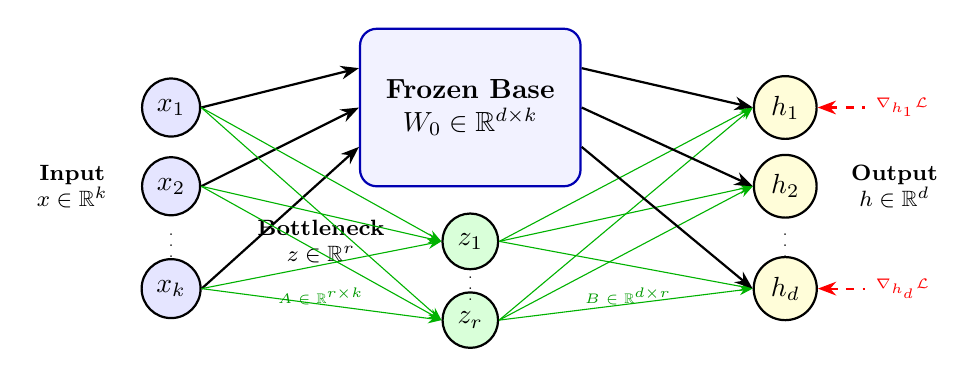
\begin{tikzpicture}[node distance=0.7cm and 1.1cm]
  \node[neuron] (x1) at (0,1.5) {$x_1$};
  \node[neuron] (x2) at (0,0.5) {$x_2$};
  \node[neuron] (xd) at (0,-0.8) {$x_k$};
  \node[font=\tiny] at (0,-0.15) {$\vdots$};
  \node[lbl, left=0.3cm of x2] {Input\\$x \in \mathbb{R}^k$};

  \node[frzblk, minimum width=2.8cm, minimum height=2.0cm] (W0) at (3.8,1.5) {\textbf{Frozen Base}\\$W_0 \in \mathbb{R}^{d \times k}$};
  \node[bneck] (z1) at (3.8,-0.2) {$z_1$};
  \node[bneck] (zr) at (3.8,-1.2) {$z_r$};
  \node[font=\tiny] at (3.8,-0.7) {$\vdots$};
  \node[lbl, left=0.6cm of z1] {Bottleneck\\$z \in \mathbb{R}^r$};

  \node[outnrn] (h1) at (7.8,1.5) {$h_1$};
  \node[outnrn] (h2) at (7.8,0.5) {$h_2$};
  \node[outnrn] (hk) at (7.8,-0.8) {$h_d$};
  \node[font=\tiny] at (7.8,-0.15) {$\vdots$};
  \node[lbl, right=0.3cm of h2] {Output\\$h \in \mathbb{R}^d$};

  \draw[arr] (x1.east) -- ($(W0.west)+(0,0.5)$);
  \draw[arr] (x2.east) -- ($(W0.west)+(0,0)$);
  \draw[arr] (xd.east) -- ($(W0.west)+(0,-0.5)$);
  \foreach \s in {x1,x2,xd} \foreach \t in {z1,zr}
    \draw[arr,green!70!black,thin] (\s.east)--(\t.west);
  \foreach \s in {z1,zr} \foreach \t in {h1,h2,hk}
    \draw[arr,green!70!black,thin] (\s.east)--(\t.west);
  \draw[arr] ($(W0.east)+(0,0.5)$)--(h1.west);
  \draw[arr] ($(W0.east)+(0,0.0)$)--(h2.west);
  \draw[arr] ($(W0.east)+(0,-0.5)$)--(hk.west);

  \node[green!60!black,font=\tiny] at (1.9,-0.9) {$A \in \mathbb{R}^{r \times k}$};
  \node[green!60!black,font=\tiny] at (5.8,-0.9) {$B \in \mathbb{R}^{d \times r}$};
  \draw[garr] (h1.east)--++(0.6,0) node[right,red,font=\tiny]{$\nabla_{h_1} \mathcal{L}$};
  \draw[garr] (hk.east)--++(0.6,0) node[right,red,font=\tiny]{$\nabla_{h_d} \mathcal{L}$};
\end{tikzpicture}
\end{adjustbox}
\caption{LoRA computational graph detailing parallel base and adapter paths and gradient backpropagation.}
\end{figure}

\subsection{Analytical Derivation of Gradients}
Let the incoming gradient with respect to the output layer be $\nabla_h \mathcal{L} = \frac{\partial \mathcal{L}}{\partial h} \in \mathbb{R}^{d \times 1}$. We derive the parameter gradients using the tensor chain rule.

\subsubsection{Gradient with respect to Matrix $B$}
Using the scalar chain rule for individual elements $B_{i,j}$:
\begin{equation}
  \frac{\partial \mathcal{L}}{\partial B_{i,j}} = \sum_{m=1}^d \frac{\partial \mathcal{L}}{\partial h_m} \frac{\partial h_m}{\partial B_{i,j}}
\end{equation}
Since $h_m = (W_0 x)_m + \frac{\alpha}{r} \sum_{l=1}^r B_{m,l} z_l$, the partial derivative is:
\begin{equation}
  \frac{\partial h_m}{\partial B_{i,j}} = \begin{cases} \frac{\alpha}{r} z_j & \text{if } m = i \\ 0 & \text{otherwise} \end{cases}
\end{equation}
Substituting this back yields:
\begin{equation}
  \frac{\partial \mathcal{L}}{\partial B_{i,j}} = \frac{\alpha}{r} \frac{\partial \mathcal{L}}{\partial h_i} z_j
\end{equation}
Expressing this in matrix notation as an outer product:
\begin{equation}
  \nabla_B \mathcal{L} = \frac{\alpha}{r} (\nabla_h \mathcal{L}) z^\top = \frac{\alpha}{r} (\nabla_h \mathcal{L}) x^\top A^\top \quad \in \mathbb{R}^{d \times r}
\end{equation}

\subsubsection{Gradient with respect to Bottleneck Activation $z$}
Before deriving the gradient for matrix $A$, we compute the gradient with respect to the bottleneck representations $z \in \mathbb{R}^r$:
\begin{equation}
  \frac{\partial \mathcal{L}}{\partial z_j} = \sum_{m=1}^d \frac{\partial \mathcal{L}}{\partial h_m} \frac{\partial h_m}{\partial z_j}
\end{equation}
Since $h_m = (W_0 x)_m + \frac{\alpha}{r} \sum_{l=1}^r B_{m,l} z_l$, we have:
\begin{equation}
  \frac{\partial h_m}{\partial z_j} = \frac{\alpha}{r} B_{m,j}
\end{equation}
Substituting this back gives:
\begin{equation}
  \frac{\partial \mathcal{L}}{\partial z_j} = \frac{\alpha}{r} \sum_{m=1}^d B_{m,j} \frac{\partial \mathcal{L}}{\partial h_m}
\end{equation}
In matrix notation, this corresponds to:
\begin{equation}
  \nabla_z \mathcal{L} = \frac{\alpha}{r} B^\top \nabla_h \mathcal{L} \quad \in \mathbb{R}^{r \times 1}
\end{equation}

\subsubsection{Gradient with respect to Matrix $A$}
Using the chain rule, we compute the gradient with respect to the elements of matrix $A$:
\begin{equation}
  \frac{\partial \mathcal{L}}{\partial A_{j,k}} = \sum_{i=1}^r \frac{\partial \mathcal{L}}{\partial z_i} \frac{\partial z_i}{\partial A_{j,k}}
\end{equation}
Since $z_i = \sum_{l=1}^k A_{i,l} x_l$, we have:
\begin{equation}
  \frac{\partial z_i}{\partial A_{j,k}} = \begin{cases} x_k & \text{if } i = j \\ 0 & \text{otherwise} \end{cases}
\end{equation}
This simplifies to:
\begin{equation}
  \frac{\partial \mathcal{L}}{\partial A_{j,k}} = \frac{\partial \mathcal{L}}{\partial z_j} x_k
\end{equation}
In matrix form:
\begin{equation}
  \nabla_A \mathcal{L} = (\nabla_z \mathcal{L}) x^\top = \frac{\alpha}{r} B^\top (\nabla_h \mathcal{L}) x^\top \quad \in \mathbb{R}^{r \times k}
\end{equation}

\subsubsection{Backpropagation to Input Activation $x$}
To pass the gradient back to the preceding layer, we compute the gradient with respect to the input activation vector $x \in \mathbb{R}^k$:
\begin{equation}
  \nabla_x \mathcal{L} = W_0^\top \nabla_h \mathcal{L} + A^\top \nabla_z \mathcal{L} = W_0^\top \nabla_h \mathcal{L} + \frac{\alpha}{r} A^\top B^\top \nabla_h \mathcal{L} \quad \in \mathbb{R}^{k \times 1}
\end{equation}
This shows that the backpropagated gradient is the sum of the gradient passing through the frozen base weights and the gradient passing through the low-rank adapter path.

\section{Weight Merging at Inference}
For inference, the forward equation $h = (W_0 + \frac{\alpha}{r} BA)x$ can be evaluated by merging the low-rank weights directly into the base weights. This eliminates the need to compute the parallel path, preventing any additional latency:
\begin{equation}
  W_{\text{merged}} = W_0 + \Delta W = W_0 + \frac{\alpha}{r} B A
\end{equation}
If the adapter needs to be swapped out for a different task, the merge operation can be reversed:
\begin{equation}
  W_0 = W_{\text{merged}} - \frac{\alpha}{r} B A
\end{equation}

\section{Memory Complexity Analysis}
In this section, we analyze the memory footprint of the optimizer states. We compare full fine-tuning of a base weight matrix $W_0 \in \mathbb{R}^{d \times k}$ against low-rank training of $A$ and $B$.

Let $N_{\text{base}} = d \cdot k$ be the number of base parameters, and $N_{\text{LoRA}} = r(d + k)$ be the number of LoRA parameters.

\subsection{AdamW Optimizer Memory Model}
AdamW tracks the following state elements for each trainable parameter:
\begin{enumerate}
  \item \textbf{Parameter value copy} (often stored in FP32 master weights during mixed-precision training): $4$ bytes.
  \item \textbf{First moment vector $m$ (momentum)}: $4$ bytes.
  \item \textbf{Second moment vector $v$ (variance)}: $4$ bytes.
\end{enumerate}
This results in $M_{\text{opt}} = 12$ bytes of optimizer state memory overhead per trainable parameter.

\subsection{Analytical Comparison}
\begin{table}[h]\centering
\begin{tabular}{lll}\toprule
\textbf{Metric} & \textbf{Full Fine-Tuning} & \textbf{LoRA Fine-Tuning} \\\midrule
Trainable Parameters & $d \cdot k$ & $r(d + k)$ \\
Optimizer State Memory & $12 \cdot d \cdot k$ bytes & $12 \cdot r(d + k)$ bytes \\
Parameter Storage Overhead & High (Gigabytes) & Low (Megabytes) \\
Activation Memory & Baseline & Baseline + $\mathcal{O}(b \cdot s \cdot r)$ \\
Gradient Memory & $2 \cdot d \cdot k$ bytes (FP16) & $2 \cdot r(d + k)$ bytes (FP16) \\\bottomrule
\end{tabular}
\caption{Memory complexity comparison between Full Fine-Tuning and LoRA.}
\end{table}

\noindent The memory saving ratio $\Phi$ is defined as:
\begin{equation}
  \Phi = \frac{M_{\text{LoRA}}}{M_{\text{Full}}} = \frac{r(d+k)}{d \cdot k} = r \left( \frac{1}{d} + \frac{1}{k} \right)
\end{equation}
Assuming a standard linear layer in a transformer block where $d = k = 4096$, and adapter rank $r = 8$:
\begin{equation}
  \Phi = 8 \left( \frac{1}{4096} + \frac{1}{4096} \right) = \frac{16}{4096} = \frac{1}{256} \approx 0.39\%
\end{equation}
This indicates a \textbf{256-fold reduction} (a decrease of $99.61\%$) in the memory required to store optimizer states for this weight matrix.

\newpage


\section{Detailed Operational Analysis of LoRA Variables}
To understand the execution of LoRA at a granular level, we detail the mathematical nature of each variable, how its values are derived in reality, its child-level control dial mental model, and its physical mechanism at the individual neuron level. We provide a full neuron-level highlight diagram for each variable.

\begin{enumerate}
  \item \textbf{Input Activation Vector ($x$)}:
    \begin{itemize}
      \item \textbf{Formula}: $x$ (output of previous layer)
      \item \textbf{Neuron Highlight Diagram}:

\begin{center}
\begin{adjustbox}{max width=0.85\linewidth}
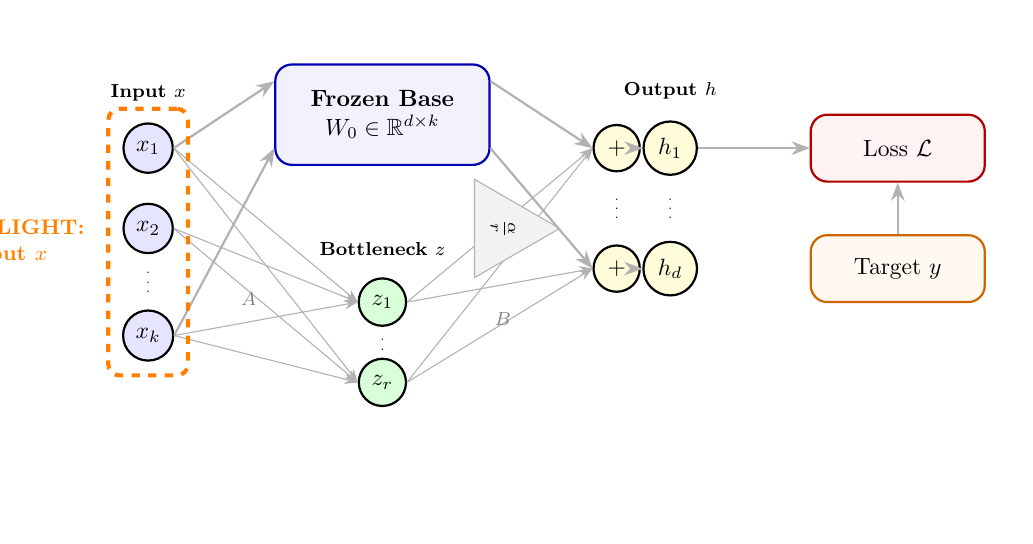
\begin{tikzpicture}[node distance=1.0cm and 1.5cm, scale=0.85, every node/.style={transform shape}]
  \useasboundingbox (-1.8, -3.5) rectangle (12.8, 3.8);
  % Input Neurons
  \node[neuron] (x1) at (0, 2) {$x_1$};
  \node[neuron] (x2) at (0, 0.8) {$x_2$};
  \node[neuron] (xk) at (0, -0.8) {$x_k$};
  \node[font=\tiny] at (0, 0.1) {$\vdots$};
  \node[lbl, above=0.2cm of x1] {Input $x$};

  % Base Weight Matrix W_0
  \node[frzblk, minimum width=3.2cm, minimum height=1.5cm] (W0) at (3.5, 2.5) {\textbf{Frozen Base} \\ $W_0 \in \mathbb{R}^{d \times k}$};

  % Bottleneck Neurons
  \node[bneck] (z1) at (3.5, -0.3) {$z_1$};
  \node[bneck] (zr) at (3.5, -1.5) {$z_r$};
  \node[font=\tiny] at (3.5, -0.9) {$\vdots$};
  \node[lbl, above=0.2cm of z1] {Bottleneck $z$};

  % Connections A
  \foreach \s in {x1,x2,xk} \foreach \t in {z1,zr}
    \draw[arr, gray!60, thin] (\s.east)--(\t.west);
  \node[text=gray, font=\footnotesize] at (1.5, -0.25) {$A$};

  % Summing Junctions and Output Neurons
  \node[sumnode] (sum1) at (7.0, 2) {$+$};
  \node[sumnode] (sumd) at (7.0, 0.2) {$+$};
  \node[font=\tiny] at (7.0, 1.2) {$\vdots$};
  
  \node[outnrn] (h1) at (7.8, 2) {$h_1$};
  \node[outnrn] (hd) at (7.8, 0.2) {$h_d$};
  \node[font=\tiny] at (7.8, 1.2) {$\vdots$};
  \node[lbl, above=0.2cm of h1] {Output $h$};

  % Connections B
  \foreach \s in {z1,zr} \foreach \t in {sum1,sumd}
    \draw[arr, gray!60, thin] (\s.east)--(\t.west);
  \node[text=gray, font=\footnotesize] at (5.3, -0.55) {$B$};

  % Scaling Multiplier
  \node[draw, regular polygon, regular polygon sides=3, rotate=-90, fill=gray!10, minimum size=0.9cm, draw=gray!60] (scale) at (5.3, 0.8) {$\frac{\alpha}{r}$};

  % Forward path connections
  \draw[arr, gray!60] (x1.east) -- ($(W0.west)+(0,0.5)$);
  \draw[arr, gray!60] (xk.east) -- ($(W0.west)+(0,-0.5)$);
  \draw[arr, gray!60] ($(W0.east)+(0,0.5)$) -- (sum1.west);
  \draw[arr, gray!60] ($(W0.east)+(0,-0.5)$) -- (sumd.west);
  \draw[arr, gray!60] (sum1) -- (h1);
  \draw[arr, gray!60] (sumd) -- (hd);

  % Loss and Target
  \node[datblk] (y) at (11.2, 0.2) {Target $y$};
  \node[lossblk] (loss) at (11.2, 2.0) {Loss $\mathcal{L}$};
  \draw[arr, gray!60] (h1.east) -- (loss.west);
  \draw[arr, gray!60] (y.north) -- (loss.south);
  
  % Dashed base outlines fit
  \node[fit=(x1) (x2) (xk)] (fit_x) {};
  \node[fit=(W0)] (fit_w0) {};
  \node[fit=(z1) (zr)] (fit_z) {};
  \node[fit=(sum1) (sumd) (h1) (hd)] (fit_h) {};

  \node[draw=orange, dashed, rounded corners=4pt, fit=(x1) (x2) (xk), inner sep=5pt, line width=1.5pt] (circle_x) {};
  \node[text=orange, font=\bfseries\small, left=0.2cm of circle_x, align=center] {HIGHLIGHT:\\Input $x$};

\end{tikzpicture}
\end{adjustbox}
\vspace{1.5em}
\end{center}

      \item \textbf{Mental Model}: Think of this vector as a list of positions for a row of thousands of physical dials. When the model processes a word, it adjusts these dials to specific numbers (e.g., dial 1 is at 4.2, dial 2 is at -1.5) to capture the meaning of the word. The model does not think in words; it thinks in these thousands of dial settings.
      \item \textbf{Neuron-Level Physical Explanation}: A single neuron in the current layer receives $x$ as a set of electrical signals from the neurons of the previous layer. Each element $x_i$ represents the activation level (firing rate) of a previous neuron after its activation function (such as ReLU or GELU). The dendrites of the current neuron receive these signals.
      \item \textbf{Mathematical Representation}: $x \in \mathbb{R}^{k \times 1}$
      \item \textbf{Code Representation}: \texttt{x} (a PyTorch tensor of shape \texttt{(batch\_size, seq\_len, k)})
      \item \textbf{Relationships}: Fed into the base projection $W_0 x$ and compressed to $z = Ax$.
    \end{itemize}

  \item \textbf{Frozen Base Weight Matrix ($W_0$)}:
    \begin{itemize}
      \item \textbf{Formula}: $W_0$
      \item \textbf{Neuron Highlight Diagram}:

\begin{center}
\begin{adjustbox}{max width=0.85\linewidth}
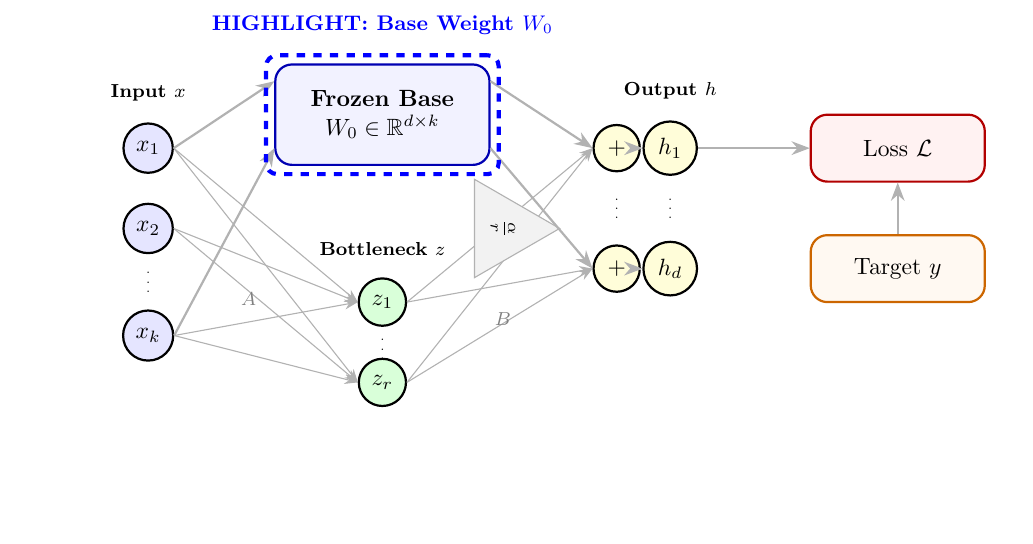
\begin{tikzpicture}[node distance=1.0cm and 1.5cm, scale=0.85, every node/.style={transform shape}]
  \useasboundingbox (-1.8, -3.5) rectangle (12.8, 3.8);
  % Input Neurons
  \node[neuron] (x1) at (0, 2) {$x_1$};
  \node[neuron] (x2) at (0, 0.8) {$x_2$};
  \node[neuron] (xk) at (0, -0.8) {$x_k$};
  \node[font=\tiny] at (0, 0.1) {$\vdots$};
  \node[lbl, above=0.2cm of x1] {Input $x$};

  % Base Weight Matrix W_0
  \node[frzblk, minimum width=3.2cm, minimum height=1.5cm] (W0) at (3.5, 2.5) {\textbf{Frozen Base} \\ $W_0 \in \mathbb{R}^{d \times k}$};

  % Bottleneck Neurons
  \node[bneck] (z1) at (3.5, -0.3) {$z_1$};
  \node[bneck] (zr) at (3.5, -1.5) {$z_r$};
  \node[font=\tiny] at (3.5, -0.9) {$\vdots$};
  \node[lbl, above=0.2cm of z1] {Bottleneck $z$};

  % Connections A
  \foreach \s in {x1,x2,xk} \foreach \t in {z1,zr}
    \draw[arr, gray!60, thin] (\s.east)--(\t.west);
  \node[text=gray, font=\footnotesize] at (1.5, -0.25) {$A$};

  % Summing Junctions and Output Neurons
  \node[sumnode] (sum1) at (7.0, 2) {$+$};
  \node[sumnode] (sumd) at (7.0, 0.2) {$+$};
  \node[font=\tiny] at (7.0, 1.2) {$\vdots$};
  
  \node[outnrn] (h1) at (7.8, 2) {$h_1$};
  \node[outnrn] (hd) at (7.8, 0.2) {$h_d$};
  \node[font=\tiny] at (7.8, 1.2) {$\vdots$};
  \node[lbl, above=0.2cm of h1] {Output $h$};

  % Connections B
  \foreach \s in {z1,zr} \foreach \t in {sum1,sumd}
    \draw[arr, gray!60, thin] (\s.east)--(\t.west);
  \node[text=gray, font=\footnotesize] at (5.3, -0.55) {$B$};

  % Scaling Multiplier
  \node[draw, regular polygon, regular polygon sides=3, rotate=-90, fill=gray!10, minimum size=0.9cm, draw=gray!60] (scale) at (5.3, 0.8) {$\frac{\alpha}{r}$};

  % Forward path connections
  \draw[arr, gray!60] (x1.east) -- ($(W0.west)+(0,0.5)$);
  \draw[arr, gray!60] (xk.east) -- ($(W0.west)+(0,-0.5)$);
  \draw[arr, gray!60] ($(W0.east)+(0,0.5)$) -- (sum1.west);
  \draw[arr, gray!60] ($(W0.east)+(0,-0.5)$) -- (sumd.west);
  \draw[arr, gray!60] (sum1) -- (h1);
  \draw[arr, gray!60] (sumd) -- (hd);

  % Loss and Target
  \node[datblk] (y) at (11.2, 0.2) {Target $y$};
  \node[lossblk] (loss) at (11.2, 2.0) {Loss $\mathcal{L}$};
  \draw[arr, gray!60] (h1.east) -- (loss.west);
  \draw[arr, gray!60] (y.north) -- (loss.south);
  
  % Dashed base outlines fit
  \node[fit=(x1) (x2) (xk)] (fit_x) {};
  \node[fit=(W0)] (fit_w0) {};
  \node[fit=(z1) (zr)] (fit_z) {};
  \node[fit=(sum1) (sumd) (h1) (hd)] (fit_h) {};

  \node[draw=blue, dashed, rounded corners=4pt, fit=(W0), inner sep=3pt, line width=1.5pt] (circle_w0) {};
  \node[text=blue, font=\bfseries\small, above=0.15cm of circle_w0] {HIGHLIGHT: Base Weight $W_0$};

\end{tikzpicture}
\end{adjustbox}
\vspace{1.5em}
\end{center}

      \item \textbf{Mental Model}: This is a giant, permanent circuit board inside the control room. The wires are soldered in place and cannot be moved (frozen). They take the positions of the incoming dials ($x$), mix them together according to the permanent rules, and output a new set of general dial positions.
      \item \textbf{Neuron-Level Physical Explanation}: A single neuron's base connections are represented by a row of $W_0$. The neuron performs a dot product: it multiplies each incoming signal $x_i$ by the strength of its corresponding synaptic connection $W_{0, ji}$ and sums them up: $y_j = \sum_i W_{0, ji} x_i$. During LoRA, these synaptic weights are frozen and cannot change, meaning their chemical/electrical conductance is locked.
      \item \textbf{Mathematical Representation}: $W_0 \in \mathbb{R}^{d \times k}$
      \item \textbf{Code Representation}: \texttt{W\_0} (a PyTorch tensor with \texttt{W\_0.requires\_grad = False} to disable gradient computation)
      \item \textbf{Relationships}: Multiplied by the input to compute the baseline representation: $h_{\text{base}} = W_0 x$.
    \end{itemize}

  \item \textbf{Down-projection Adapter ($A$)}:
    \begin{itemize}
      \item \textbf{Formula}: $A$
      \item \textbf{Neuron Highlight Diagram}:

\begin{center}
\begin{adjustbox}{max width=0.85\linewidth}
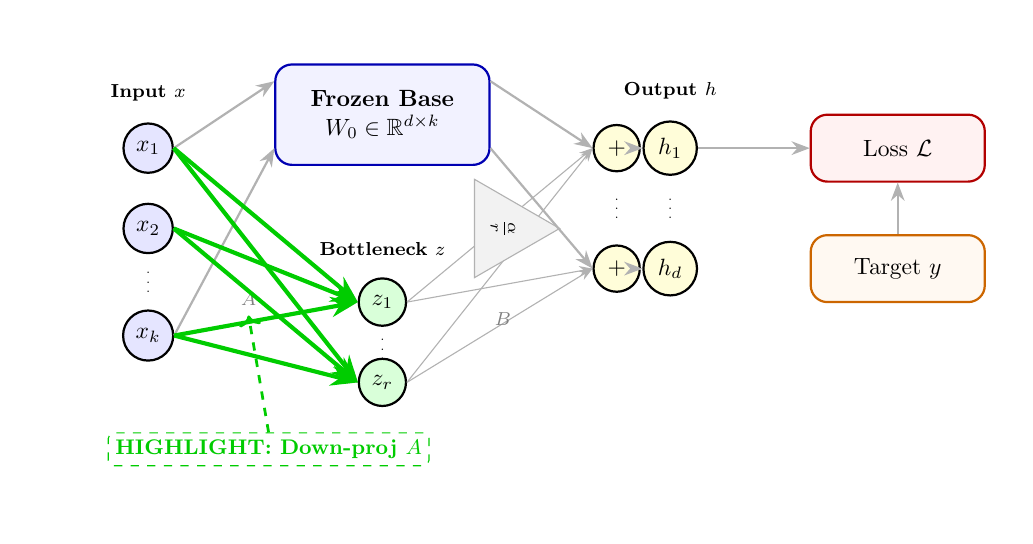
\begin{tikzpicture}[node distance=1.0cm and 1.5cm, scale=0.85, every node/.style={transform shape}]
  \useasboundingbox (-1.8, -3.5) rectangle (12.8, 3.8);
  % Input Neurons
  \node[neuron] (x1) at (0, 2) {$x_1$};
  \node[neuron] (x2) at (0, 0.8) {$x_2$};
  \node[neuron] (xk) at (0, -0.8) {$x_k$};
  \node[font=\tiny] at (0, 0.1) {$\vdots$};
  \node[lbl, above=0.2cm of x1] {Input $x$};

  % Base Weight Matrix W_0
  \node[frzblk, minimum width=3.2cm, minimum height=1.5cm] (W0) at (3.5, 2.5) {\textbf{Frozen Base} \\ $W_0 \in \mathbb{R}^{d \times k}$};

  % Bottleneck Neurons
  \node[bneck] (z1) at (3.5, -0.3) {$z_1$};
  \node[bneck] (zr) at (3.5, -1.5) {$z_r$};
  \node[font=\tiny] at (3.5, -0.9) {$\vdots$};
  \node[lbl, above=0.2cm of z1] {Bottleneck $z$};

  % Connections A
  \foreach \s in {x1,x2,xk} \foreach \t in {z1,zr}
    \draw[arr, gray!60, thin] (\s.east)--(\t.west);
  \node[text=gray, font=\footnotesize] at (1.5, -0.25) {$A$};

  % Summing Junctions and Output Neurons
  \node[sumnode] (sum1) at (7.0, 2) {$+$};
  \node[sumnode] (sumd) at (7.0, 0.2) {$+$};
  \node[font=\tiny] at (7.0, 1.2) {$\vdots$};
  
  \node[outnrn] (h1) at (7.8, 2) {$h_1$};
  \node[outnrn] (hd) at (7.8, 0.2) {$h_d$};
  \node[font=\tiny] at (7.8, 1.2) {$\vdots$};
  \node[lbl, above=0.2cm of h1] {Output $h$};

  % Connections B
  \foreach \s in {z1,zr} \foreach \t in {sum1,sumd}
    \draw[arr, gray!60, thin] (\s.east)--(\t.west);
  \node[text=gray, font=\footnotesize] at (5.3, -0.55) {$B$};

  % Scaling Multiplier
  \node[draw, regular polygon, regular polygon sides=3, rotate=-90, fill=gray!10, minimum size=0.9cm, draw=gray!60] (scale) at (5.3, 0.8) {$\frac{\alpha}{r}$};

  % Forward path connections
  \draw[arr, gray!60] (x1.east) -- ($(W0.west)+(0,0.5)$);
  \draw[arr, gray!60] (xk.east) -- ($(W0.west)+(0,-0.5)$);
  \draw[arr, gray!60] ($(W0.east)+(0,0.5)$) -- (sum1.west);
  \draw[arr, gray!60] ($(W0.east)+(0,-0.5)$) -- (sumd.west);
  \draw[arr, gray!60] (sum1) -- (h1);
  \draw[arr, gray!60] (sumd) -- (hd);

  % Loss and Target
  \node[datblk] (y) at (11.2, 0.2) {Target $y$};
  \node[lossblk] (loss) at (11.2, 2.0) {Loss $\mathcal{L}$};
  \draw[arr, gray!60] (h1.east) -- (loss.west);
  \draw[arr, gray!60] (y.north) -- (loss.south);
  
  % Dashed base outlines fit
  \node[fit=(x1) (x2) (xk)] (fit_x) {};
  \node[fit=(W0)] (fit_w0) {};
  \node[fit=(z1) (zr)] (fit_z) {};
  \node[fit=(sum1) (sumd) (h1) (hd)] (fit_h) {};

  \foreach \s in {x1,x2,xk} \foreach \t in {z1,zr}
    \draw[arr, green!80!black, line width=1.5pt] (\s.east)--(\t.west);
  \node[text=green!80!black, font=\bfseries\small, draw=green!80!black, dashed, inner sep=3pt, rounded corners=2pt, fill=white] (lbl_A) at (1.8, -2.5) {HIGHLIGHT: Down-proj $A$};
  \draw[dashed, green!80!black, line width=1pt, ->] (lbl_A.north) -- (1.5, -0.5);

\end{tikzpicture}
\end{adjustbox}
\vspace{1.5em}
\end{center}

      \item \textbf{Mental Model}: This is a smaller circuit board that acts as a compression funnel. It looks at all the thousands of input dials and summarizes them into just a few dials (e.g., summarizing $4096$ dials into just $8$ dials). It only listens to the dial changes that are relevant to the new task we are teaching the model.
      \item \textbf{Neuron-Level Physical Explanation}: Inside the adapter path, a single neuron in the bottleneck layer corresponds to a row of matrix $A$. This neuron listens to all input signals $x_i$, multiplies them by its trainable weights $A_{mi}$, and sums them up: $z_m = \sum_i A_{mi} x_i$. This bottleneck neuron acts as a feature detector that extracts a specific combination of input signals.
      \item \textbf{Mathematical Representation}: $A \in \mathbb{R}^{r \times k}$
      \item \textbf{Code Representation}: \texttt{A} (initialized as \texttt{nn.Linear(}k, r, bias=False) with weight values drawn from a Gaussian distribution: \texttt{nn.init.kaiming\_uniform\_(A.weight, a=math.sqrt(5))})
      \item \textbf{Relationships}: Compresses $x$ into the bottleneck space via $z = Ax$.
    \end{itemize}

  \item \textbf{Up-projection Adapter ($B$)}:
    \begin{itemize}
      \item \textbf{Formula}: $B$
      \item \textbf{Neuron Highlight Diagram}:

\begin{center}
\begin{adjustbox}{max width=0.85\linewidth}
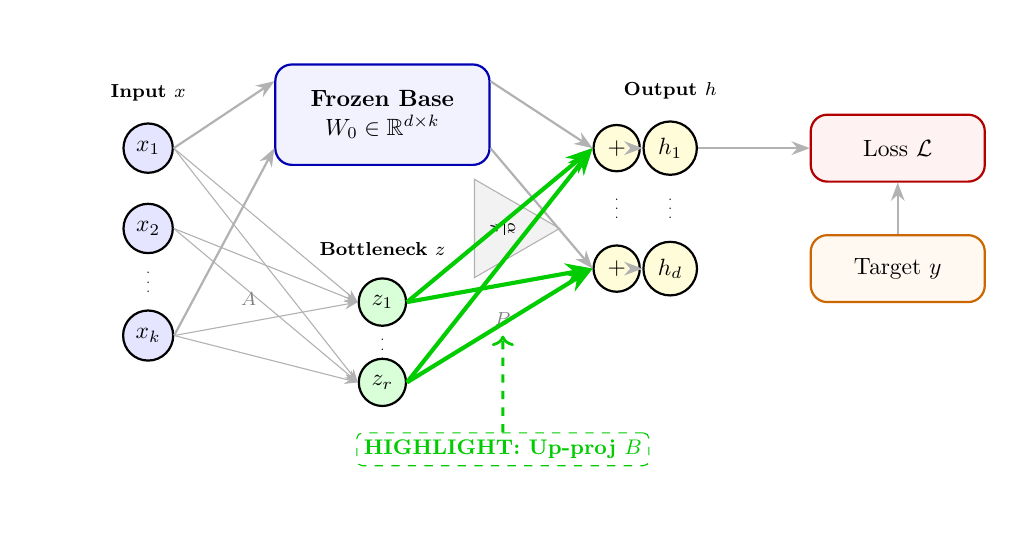
\begin{tikzpicture}[node distance=1.0cm and 1.5cm, scale=0.85, every node/.style={transform shape}]
  \useasboundingbox (-1.8, -3.5) rectangle (12.8, 3.8);
  % Input Neurons
  \node[neuron] (x1) at (0, 2) {$x_1$};
  \node[neuron] (x2) at (0, 0.8) {$x_2$};
  \node[neuron] (xk) at (0, -0.8) {$x_k$};
  \node[font=\tiny] at (0, 0.1) {$\vdots$};
  \node[lbl, above=0.2cm of x1] {Input $x$};

  % Base Weight Matrix W_0
  \node[frzblk, minimum width=3.2cm, minimum height=1.5cm] (W0) at (3.5, 2.5) {\textbf{Frozen Base} \\ $W_0 \in \mathbb{R}^{d \times k}$};

  % Bottleneck Neurons
  \node[bneck] (z1) at (3.5, -0.3) {$z_1$};
  \node[bneck] (zr) at (3.5, -1.5) {$z_r$};
  \node[font=\tiny] at (3.5, -0.9) {$\vdots$};
  \node[lbl, above=0.2cm of z1] {Bottleneck $z$};

  % Connections A
  \foreach \s in {x1,x2,xk} \foreach \t in {z1,zr}
    \draw[arr, gray!60, thin] (\s.east)--(\t.west);
  \node[text=gray, font=\footnotesize] at (1.5, -0.25) {$A$};

  % Summing Junctions and Output Neurons
  \node[sumnode] (sum1) at (7.0, 2) {$+$};
  \node[sumnode] (sumd) at (7.0, 0.2) {$+$};
  \node[font=\tiny] at (7.0, 1.2) {$\vdots$};
  
  \node[outnrn] (h1) at (7.8, 2) {$h_1$};
  \node[outnrn] (hd) at (7.8, 0.2) {$h_d$};
  \node[font=\tiny] at (7.8, 1.2) {$\vdots$};
  \node[lbl, above=0.2cm of h1] {Output $h$};

  % Connections B
  \foreach \s in {z1,zr} \foreach \t in {sum1,sumd}
    \draw[arr, gray!60, thin] (\s.east)--(\t.west);
  \node[text=gray, font=\footnotesize] at (5.3, -0.55) {$B$};

  % Scaling Multiplier
  \node[draw, regular polygon, regular polygon sides=3, rotate=-90, fill=gray!10, minimum size=0.9cm, draw=gray!60] (scale) at (5.3, 0.8) {$\frac{\alpha}{r}$};

  % Forward path connections
  \draw[arr, gray!60] (x1.east) -- ($(W0.west)+(0,0.5)$);
  \draw[arr, gray!60] (xk.east) -- ($(W0.west)+(0,-0.5)$);
  \draw[arr, gray!60] ($(W0.east)+(0,0.5)$) -- (sum1.west);
  \draw[arr, gray!60] ($(W0.east)+(0,-0.5)$) -- (sumd.west);
  \draw[arr, gray!60] (sum1) -- (h1);
  \draw[arr, gray!60] (sumd) -- (hd);

  % Loss and Target
  \node[datblk] (y) at (11.2, 0.2) {Target $y$};
  \node[lossblk] (loss) at (11.2, 2.0) {Loss $\mathcal{L}$};
  \draw[arr, gray!60] (h1.east) -- (loss.west);
  \draw[arr, gray!60] (y.north) -- (loss.south);
  
  % Dashed base outlines fit
  \node[fit=(x1) (x2) (xk)] (fit_x) {};
  \node[fit=(W0)] (fit_w0) {};
  \node[fit=(z1) (zr)] (fit_z) {};
  \node[fit=(sum1) (sumd) (h1) (hd)] (fit_h) {};

  \foreach \s in {z1,zr} \foreach \t in {sum1,sumd}
    \draw[arr, green!80!black, line width=1.5pt] (\s.east)--(\t.west);
  \node[text=green!80!black, font=\bfseries\small, draw=green!80!black, dashed, inner sep=3pt, rounded corners=2pt, fill=white] (lbl_B) at (5.3, -2.5) {HIGHLIGHT: Up-proj $B$};
  \draw[dashed, green!80!black, line width=1pt, ->] (lbl_B.north) -- (5.3, -0.8);

\end{tikzpicture}
\end{adjustbox}
\vspace{1.5em}
\end{center}

      \item \textbf{Mental Model}: This is another small circuit board that acts as an expansion nozzle. It takes the tiny summary from the funnel (our $8$ dials) and expands it back into thousands of dials, showing how to nudge the final output dials to fit the new task.
      \item \textbf{Neuron-Level Physical Explanation}: A single output neuron receives contributions from the bottleneck neurons. The connection strength from bottleneck neuron $m$ to output neuron $j$ is the trainable weight $B_{jm}$. The output neuron sums the weighted signals from all bottleneck neurons: $u_j = \sum_m B_{jm} z_m$, scaling up the low-dimensional task features.
      \item \textbf{Mathematical Representation}: $B \in \mathbb{R}^{d \times r}$
      \item \textbf{Code Representation}: \texttt{B} (initialized as \texttt{nn.Linear(r, }d, bias=False) with weight values set to all zeros: \texttt{nn.init.zeros\_(B.weight)})
      \item \textbf{Relationships}: Expands the bottleneck activations via $B z$, scaled by $\frac{\alpha}{r}$.
    \end{itemize}

  \item \textbf{Bottleneck Rank ($r$)}:
    \begin{itemize}
      \item \textbf{Formula}: $r$
      \item \textbf{Neuron Highlight Diagram}:

\begin{center}
\begin{adjustbox}{max width=0.85\linewidth}
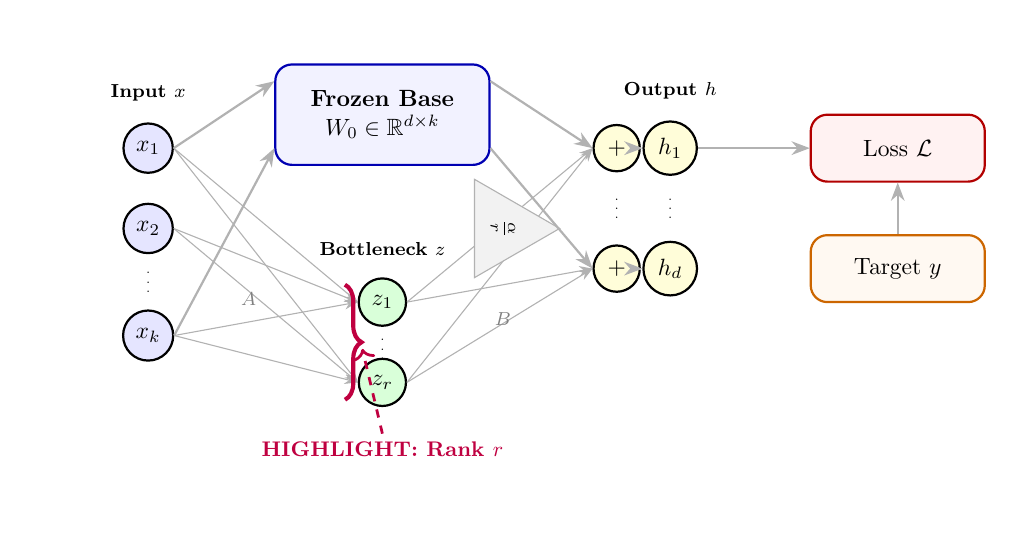
\begin{tikzpicture}[node distance=1.0cm and 1.5cm, scale=0.85, every node/.style={transform shape}]
  \useasboundingbox (-1.8, -3.5) rectangle (12.8, 3.8);
  % Input Neurons
  \node[neuron] (x1) at (0, 2) {$x_1$};
  \node[neuron] (x2) at (0, 0.8) {$x_2$};
  \node[neuron] (xk) at (0, -0.8) {$x_k$};
  \node[font=\tiny] at (0, 0.1) {$\vdots$};
  \node[lbl, above=0.2cm of x1] {Input $x$};

  % Base Weight Matrix W_0
  \node[frzblk, minimum width=3.2cm, minimum height=1.5cm] (W0) at (3.5, 2.5) {\textbf{Frozen Base} \\ $W_0 \in \mathbb{R}^{d \times k}$};

  % Bottleneck Neurons
  \node[bneck] (z1) at (3.5, -0.3) {$z_1$};
  \node[bneck] (zr) at (3.5, -1.5) {$z_r$};
  \node[font=\tiny] at (3.5, -0.9) {$\vdots$};
  \node[lbl, above=0.2cm of z1] {Bottleneck $z$};

  % Connections A
  \foreach \s in {x1,x2,xk} \foreach \t in {z1,zr}
    \draw[arr, gray!60, thin] (\s.east)--(\t.west);
  \node[text=gray, font=\footnotesize] at (1.5, -0.25) {$A$};

  % Summing Junctions and Output Neurons
  \node[sumnode] (sum1) at (7.0, 2) {$+$};
  \node[sumnode] (sumd) at (7.0, 0.2) {$+$};
  \node[font=\tiny] at (7.0, 1.2) {$\vdots$};
  
  \node[outnrn] (h1) at (7.8, 2) {$h_1$};
  \node[outnrn] (hd) at (7.8, 0.2) {$h_d$};
  \node[font=\tiny] at (7.8, 1.2) {$\vdots$};
  \node[lbl, above=0.2cm of h1] {Output $h$};

  % Connections B
  \foreach \s in {z1,zr} \foreach \t in {sum1,sumd}
    \draw[arr, gray!60, thin] (\s.east)--(\t.west);
  \node[text=gray, font=\footnotesize] at (5.3, -0.55) {$B$};

  % Scaling Multiplier
  \node[draw, regular polygon, regular polygon sides=3, rotate=-90, fill=gray!10, minimum size=0.9cm, draw=gray!60] (scale) at (5.3, 0.8) {$\frac{\alpha}{r}$};

  % Forward path connections
  \draw[arr, gray!60] (x1.east) -- ($(W0.west)+(0,0.5)$);
  \draw[arr, gray!60] (xk.east) -- ($(W0.west)+(0,-0.5)$);
  \draw[arr, gray!60] ($(W0.east)+(0,0.5)$) -- (sum1.west);
  \draw[arr, gray!60] ($(W0.east)+(0,-0.5)$) -- (sumd.west);
  \draw[arr, gray!60] (sum1) -- (h1);
  \draw[arr, gray!60] (sumd) -- (hd);

  % Loss and Target
  \node[datblk] (y) at (11.2, 0.2) {Target $y$};
  \node[lossblk] (loss) at (11.2, 2.0) {Loss $\mathcal{L}$};
  \draw[arr, gray!60] (h1.east) -- (loss.west);
  \draw[arr, gray!60] (y.north) -- (loss.south);
  
  % Dashed base outlines fit
  \node[fit=(x1) (x2) (xk)] (fit_x) {};
  \node[fit=(W0)] (fit_w0) {};
  \node[fit=(z1) (zr)] (fit_z) {};
  \node[fit=(sum1) (sumd) (h1) (hd)] (fit_h) {};

  \draw[decoration={brace,mirror,amplitude=6pt},decorate,line width=1.5pt,draw=purple] ($(zr.south west)+(-0.3,0)$) -- ($(z1.north west)+(-0.3,0)$);
  \node[text=purple, font=\bfseries\small] (lbl_r) at (3.5, -2.5) {HIGHLIGHT: Rank $r$};
  \draw[dashed, purple, line width=1pt, ->] (lbl_r.north) -- (3.2, -1.0);

\end{tikzpicture}
\end{adjustbox}
\vspace{1.5em}
\end{center}

      \item \textbf{Mental Model}: This is the exact number of summary dials inside the bottleneck. If $r=8$, it means we are forcing the model to summarize all its knowledge into just $8$ dials. A smaller number makes the funnel tighter, forcing the model to only keep the most important summaries.
      \item \textbf{Neuron-Level Physical Explanation}: This is the exact number of neurons present in the bottleneck layer of the adapter. Selecting $r=8$ means there are exactly 8 neurons in this intermediate layer. Each of these 8 neurons acts as a specialized task detector.
      \item \textbf{Mathematical Representation}: $r \in \mathbb{Z}^{+}$
      \item \textbf{Code Representation}: \texttt{r} (passed as an integer configuration parameter, e.g., \texttt{lora\_config = LoraConfig(r=8)})
      \item \textbf{Relationships}: Determines the inner dimension of matrices $A$ and $B$, and acts as a scaling denominator in $\frac{\alpha}{r}$.
    \end{itemize}

  \item \textbf{Scaling Constant ($\alpha$)}:
    \begin{itemize}
      \item \textbf{Formula}: $\alpha$
      \item \textbf{Neuron Highlight Diagram}:

\begin{center}
\begin{adjustbox}{max width=0.85\linewidth}
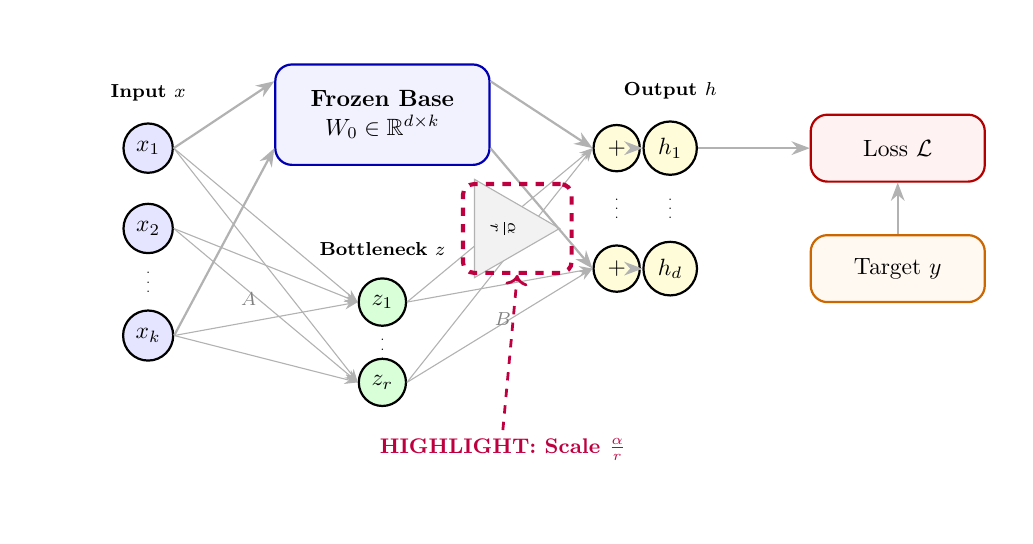
\begin{tikzpicture}[node distance=1.0cm and 1.5cm, scale=0.85, every node/.style={transform shape}]
  \useasboundingbox (-1.8, -3.5) rectangle (12.8, 3.8);
  % Input Neurons
  \node[neuron] (x1) at (0, 2) {$x_1$};
  \node[neuron] (x2) at (0, 0.8) {$x_2$};
  \node[neuron] (xk) at (0, -0.8) {$x_k$};
  \node[font=\tiny] at (0, 0.1) {$\vdots$};
  \node[lbl, above=0.2cm of x1] {Input $x$};

  % Base Weight Matrix W_0
  \node[frzblk, minimum width=3.2cm, minimum height=1.5cm] (W0) at (3.5, 2.5) {\textbf{Frozen Base} \\ $W_0 \in \mathbb{R}^{d \times k}$};

  % Bottleneck Neurons
  \node[bneck] (z1) at (3.5, -0.3) {$z_1$};
  \node[bneck] (zr) at (3.5, -1.5) {$z_r$};
  \node[font=\tiny] at (3.5, -0.9) {$\vdots$};
  \node[lbl, above=0.2cm of z1] {Bottleneck $z$};

  % Connections A
  \foreach \s in {x1,x2,xk} \foreach \t in {z1,zr}
    \draw[arr, gray!60, thin] (\s.east)--(\t.west);
  \node[text=gray, font=\footnotesize] at (1.5, -0.25) {$A$};

  % Summing Junctions and Output Neurons
  \node[sumnode] (sum1) at (7.0, 2) {$+$};
  \node[sumnode] (sumd) at (7.0, 0.2) {$+$};
  \node[font=\tiny] at (7.0, 1.2) {$\vdots$};
  
  \node[outnrn] (h1) at (7.8, 2) {$h_1$};
  \node[outnrn] (hd) at (7.8, 0.2) {$h_d$};
  \node[font=\tiny] at (7.8, 1.2) {$\vdots$};
  \node[lbl, above=0.2cm of h1] {Output $h$};

  % Connections B
  \foreach \s in {z1,zr} \foreach \t in {sum1,sumd}
    \draw[arr, gray!60, thin] (\s.east)--(\t.west);
  \node[text=gray, font=\footnotesize] at (5.3, -0.55) {$B$};

  % Scaling Multiplier
  \node[draw, regular polygon, regular polygon sides=3, rotate=-90, fill=gray!10, minimum size=0.9cm, draw=gray!60] (scale) at (5.3, 0.8) {$\frac{\alpha}{r}$};

  % Forward path connections
  \draw[arr, gray!60] (x1.east) -- ($(W0.west)+(0,0.5)$);
  \draw[arr, gray!60] (xk.east) -- ($(W0.west)+(0,-0.5)$);
  \draw[arr, gray!60] ($(W0.east)+(0,0.5)$) -- (sum1.west);
  \draw[arr, gray!60] ($(W0.east)+(0,-0.5)$) -- (sumd.west);
  \draw[arr, gray!60] (sum1) -- (h1);
  \draw[arr, gray!60] (sumd) -- (hd);

  % Loss and Target
  \node[datblk] (y) at (11.2, 0.2) {Target $y$};
  \node[lossblk] (loss) at (11.2, 2.0) {Loss $\mathcal{L}$};
  \draw[arr, gray!60] (h1.east) -- (loss.west);
  \draw[arr, gray!60] (y.north) -- (loss.south);
  
  % Dashed base outlines fit
  \node[fit=(x1) (x2) (xk)] (fit_x) {};
  \node[fit=(W0)] (fit_w0) {};
  \node[fit=(z1) (zr)] (fit_z) {};
  \node[fit=(sum1) (sumd) (h1) (hd)] (fit_h) {};

  \node[draw=purple, dashed, rounded corners=4pt, fit=(scale), inner sep=4pt, line width=1.5pt] (circle_scale) {};
  \node[text=purple, font=\bfseries\small] (lbl_scale) at (5.3, -2.5) {HIGHLIGHT: Scale $\frac{\alpha}{r}$};
  \draw[dashed, purple, line width=1pt, ->] (lbl_scale.north) -- (circle_scale.south);

\end{tikzpicture}
\end{adjustbox}
\vspace{1.5em}
\end{center}

      \item \textbf{Mental Model}: This is a volume control knob. It decides how loudly the changes from the new adapters ($A$ and $B$) should shout compared to the original, permanent circuit board ($W_0$). If we turn this knob up, the model listens more to its new training and less to its old pretrained knowledge.
      \item \textbf{Neuron-Level Physical Explanation}: At the neuron level, this acts as a synaptic gain control. The signal coming from the bottleneck via the adapter pathway is amplified or attenuated by a constant scale factor of $\frac{\alpha}{r}$ before it is added to the base neuron's output. This behaves like a biological neuromodulator that globally scales the synaptic sensitivity of the adapter path.
      \item \textbf{Mathematical Representation}: $\alpha \in \mathbb{R}^{+}$
      \item \textbf{Code Representation}: \texttt{lora\_alpha} (passed as a configuration parameter, e.g., \texttt{lora\_config = LoraConfig(lora\_alpha=16)})
      \item \textbf{Relationships}: Multiplies the adapter pathway output, yielding $\frac{\alpha}{r} B z$.
    \end{itemize}

  \item \textbf{Bottleneck Activation Vector ($z$)}:
    \begin{itemize}
      \item \textbf{Formula}: $z = Ax$
      \item \textbf{Neuron Highlight Diagram}:

\begin{center}
\begin{adjustbox}{max width=0.85\linewidth}
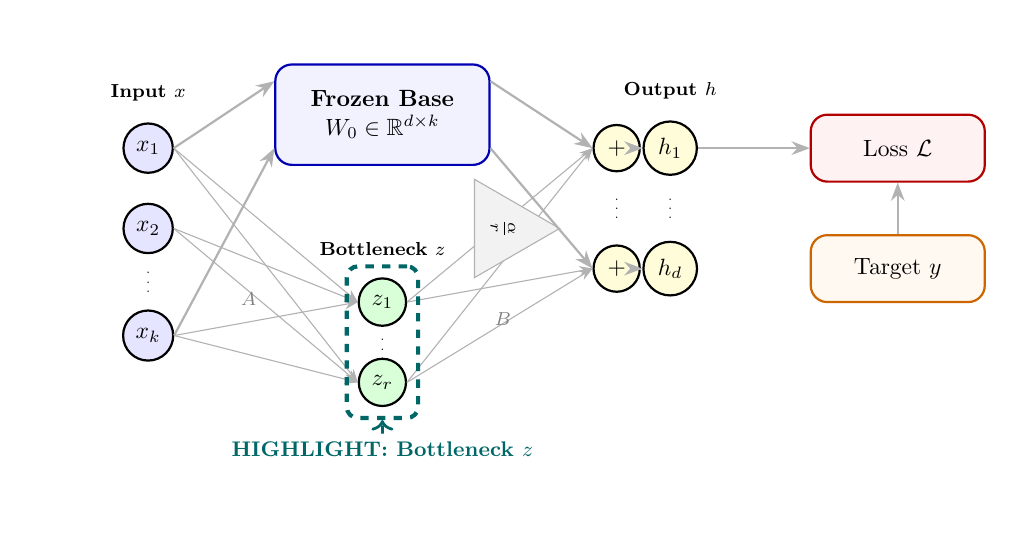
\begin{tikzpicture}[node distance=1.0cm and 1.5cm, scale=0.85, every node/.style={transform shape}]
  \useasboundingbox (-1.8, -3.5) rectangle (12.8, 3.8);
  % Input Neurons
  \node[neuron] (x1) at (0, 2) {$x_1$};
  \node[neuron] (x2) at (0, 0.8) {$x_2$};
  \node[neuron] (xk) at (0, -0.8) {$x_k$};
  \node[font=\tiny] at (0, 0.1) {$\vdots$};
  \node[lbl, above=0.2cm of x1] {Input $x$};

  % Base Weight Matrix W_0
  \node[frzblk, minimum width=3.2cm, minimum height=1.5cm] (W0) at (3.5, 2.5) {\textbf{Frozen Base} \\ $W_0 \in \mathbb{R}^{d \times k}$};

  % Bottleneck Neurons
  \node[bneck] (z1) at (3.5, -0.3) {$z_1$};
  \node[bneck] (zr) at (3.5, -1.5) {$z_r$};
  \node[font=\tiny] at (3.5, -0.9) {$\vdots$};
  \node[lbl, above=0.2cm of z1] {Bottleneck $z$};

  % Connections A
  \foreach \s in {x1,x2,xk} \foreach \t in {z1,zr}
    \draw[arr, gray!60, thin] (\s.east)--(\t.west);
  \node[text=gray, font=\footnotesize] at (1.5, -0.25) {$A$};

  % Summing Junctions and Output Neurons
  \node[sumnode] (sum1) at (7.0, 2) {$+$};
  \node[sumnode] (sumd) at (7.0, 0.2) {$+$};
  \node[font=\tiny] at (7.0, 1.2) {$\vdots$};
  
  \node[outnrn] (h1) at (7.8, 2) {$h_1$};
  \node[outnrn] (hd) at (7.8, 0.2) {$h_d$};
  \node[font=\tiny] at (7.8, 1.2) {$\vdots$};
  \node[lbl, above=0.2cm of h1] {Output $h$};

  % Connections B
  \foreach \s in {z1,zr} \foreach \t in {sum1,sumd}
    \draw[arr, gray!60, thin] (\s.east)--(\t.west);
  \node[text=gray, font=\footnotesize] at (5.3, -0.55) {$B$};

  % Scaling Multiplier
  \node[draw, regular polygon, regular polygon sides=3, rotate=-90, fill=gray!10, minimum size=0.9cm, draw=gray!60] (scale) at (5.3, 0.8) {$\frac{\alpha}{r}$};

  % Forward path connections
  \draw[arr, gray!60] (x1.east) -- ($(W0.west)+(0,0.5)$);
  \draw[arr, gray!60] (xk.east) -- ($(W0.west)+(0,-0.5)$);
  \draw[arr, gray!60] ($(W0.east)+(0,0.5)$) -- (sum1.west);
  \draw[arr, gray!60] ($(W0.east)+(0,-0.5)$) -- (sumd.west);
  \draw[arr, gray!60] (sum1) -- (h1);
  \draw[arr, gray!60] (sumd) -- (hd);

  % Loss and Target
  \node[datblk] (y) at (11.2, 0.2) {Target $y$};
  \node[lossblk] (loss) at (11.2, 2.0) {Loss $\mathcal{L}$};
  \draw[arr, gray!60] (h1.east) -- (loss.west);
  \draw[arr, gray!60] (y.north) -- (loss.south);
  
  % Dashed base outlines fit
  \node[fit=(x1) (x2) (xk)] (fit_x) {};
  \node[fit=(W0)] (fit_w0) {};
  \node[fit=(z1) (zr)] (fit_z) {};
  \node[fit=(sum1) (sumd) (h1) (hd)] (fit_h) {};

  \node[draw=teal!80!black, dashed, rounded corners=4pt, fit=(z1) (zr), inner sep=4pt, line width=1.5pt] (circle_z) {};
  \node[text=teal!80!black, font=\bfseries\small] (lbl_z) at (3.5, -2.5) {HIGHLIGHT: Bottleneck $z$};
  \draw[dashed, teal!80!black, line width=1pt, ->] (lbl_z.north) -- (circle_z.south);

\end{tikzpicture}
\end{adjustbox}
\vspace{1.5em}
\end{center}

      \item \textbf{Mental Model}: These are the actual values of our few summary dials inside the bottleneck. It represents the compressed task-specific message as it flows from the compression funnel to the expansion nozzle.
      \item \textbf{Neuron-Level Physical Explanation}: Each element $z_m$ is the electrical activation level (firing rate) of a single neuron in the bottleneck layer. It is calculated by that neuron summing its inputs: $z_m = \sum_i A_{mi} x_i$.
      \item \textbf{Mathematical Representation}: $z \in \mathbb{R}^{r \times 1}$
      \item \textbf{Code Representation}: \texttt{z = F.linear(x, A.weight)} (or \texttt{z = x @ A.weight.t()})
      \item \textbf{Relationships}: Created by $A$, consumed by $B$.
    \end{itemize}

  \item \textbf{Combined Output Vector ($h$)}:
    \begin{itemize}
      \item \textbf{Formula}: $h = W_0 x + \frac{\alpha}{r} B z$
      \item \textbf{Neuron Highlight Diagram}:

\begin{center}
\begin{adjustbox}{max width=0.85\linewidth}
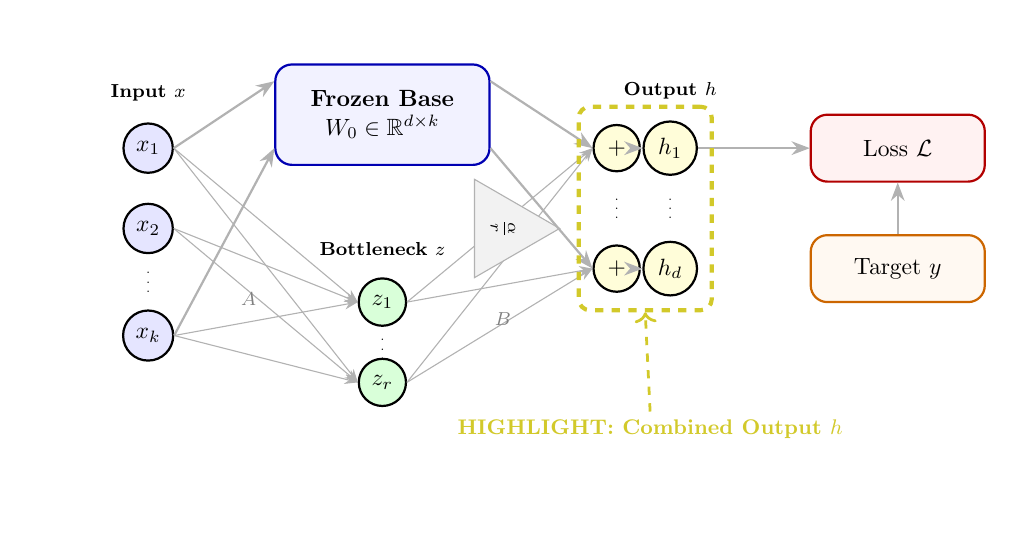
\begin{tikzpicture}[node distance=1.0cm and 1.5cm, scale=0.85, every node/.style={transform shape}]
  \useasboundingbox (-1.8, -3.5) rectangle (12.8, 3.8);
  % Input Neurons
  \node[neuron] (x1) at (0, 2) {$x_1$};
  \node[neuron] (x2) at (0, 0.8) {$x_2$};
  \node[neuron] (xk) at (0, -0.8) {$x_k$};
  \node[font=\tiny] at (0, 0.1) {$\vdots$};
  \node[lbl, above=0.2cm of x1] {Input $x$};

  % Base Weight Matrix W_0
  \node[frzblk, minimum width=3.2cm, minimum height=1.5cm] (W0) at (3.5, 2.5) {\textbf{Frozen Base} \\ $W_0 \in \mathbb{R}^{d \times k}$};

  % Bottleneck Neurons
  \node[bneck] (z1) at (3.5, -0.3) {$z_1$};
  \node[bneck] (zr) at (3.5, -1.5) {$z_r$};
  \node[font=\tiny] at (3.5, -0.9) {$\vdots$};
  \node[lbl, above=0.2cm of z1] {Bottleneck $z$};

  % Connections A
  \foreach \s in {x1,x2,xk} \foreach \t in {z1,zr}
    \draw[arr, gray!60, thin] (\s.east)--(\t.west);
  \node[text=gray, font=\footnotesize] at (1.5, -0.25) {$A$};

  % Summing Junctions and Output Neurons
  \node[sumnode] (sum1) at (7.0, 2) {$+$};
  \node[sumnode] (sumd) at (7.0, 0.2) {$+$};
  \node[font=\tiny] at (7.0, 1.2) {$\vdots$};
  
  \node[outnrn] (h1) at (7.8, 2) {$h_1$};
  \node[outnrn] (hd) at (7.8, 0.2) {$h_d$};
  \node[font=\tiny] at (7.8, 1.2) {$\vdots$};
  \node[lbl, above=0.2cm of h1] {Output $h$};

  % Connections B
  \foreach \s in {z1,zr} \foreach \t in {sum1,sumd}
    \draw[arr, gray!60, thin] (\s.east)--(\t.west);
  \node[text=gray, font=\footnotesize] at (5.3, -0.55) {$B$};

  % Scaling Multiplier
  \node[draw, regular polygon, regular polygon sides=3, rotate=-90, fill=gray!10, minimum size=0.9cm, draw=gray!60] (scale) at (5.3, 0.8) {$\frac{\alpha}{r}$};

  % Forward path connections
  \draw[arr, gray!60] (x1.east) -- ($(W0.west)+(0,0.5)$);
  \draw[arr, gray!60] (xk.east) -- ($(W0.west)+(0,-0.5)$);
  \draw[arr, gray!60] ($(W0.east)+(0,0.5)$) -- (sum1.west);
  \draw[arr, gray!60] ($(W0.east)+(0,-0.5)$) -- (sumd.west);
  \draw[arr, gray!60] (sum1) -- (h1);
  \draw[arr, gray!60] (sumd) -- (hd);

  % Loss and Target
  \node[datblk] (y) at (11.2, 0.2) {Target $y$};
  \node[lossblk] (loss) at (11.2, 2.0) {Loss $\mathcal{L}$};
  \draw[arr, gray!60] (h1.east) -- (loss.west);
  \draw[arr, gray!60] (y.north) -- (loss.south);
  
  % Dashed base outlines fit
  \node[fit=(x1) (x2) (xk)] (fit_x) {};
  \node[fit=(W0)] (fit_w0) {};
  \node[fit=(z1) (zr)] (fit_z) {};
  \node[fit=(sum1) (sumd) (h1) (hd)] (fit_h) {};

  \node[draw=yellow!80!black, dashed, rounded corners=4pt, fit=(sum1) (sumd) (h1) (hd), inner sep=5pt, line width=1.5pt] (circle_h) {};
  \node[text=yellow!80!black, font=\bfseries\small] (lbl_h) at (7.5, -2.2) {HIGHLIGHT: Combined Output $h$};
  \draw[dashed, yellow!80!black, line width=1pt, ->] (lbl_h.north) -- (circle_h.south);

\end{tikzpicture}
\end{adjustbox}
\vspace{1.5em}
\end{center}

      \item \textbf{Mental Model}: This is the final row of output dials. It is created by taking the general dial settings computed by the permanent circuit board ($W_0$) and nudging them slightly using the task-specific dial settings computed by our adapters.
      \item \textbf{Neuron-Level Physical Explanation}: A single output neuron $j$ sums the signals from the frozen base connection path and the scaled trainable adapter path: $h_j = \sum_i W_{0, ji} x_i + \frac{\alpha}{r} \sum_m B_{jm} z_m$. The neuron acts as a physical summing junction, integrating the general-purpose signal and the specialized task signal.
      \item \textbf{Mathematical Representation}: $h \in \mathbb{R}^{d \times 1}$
      \item \textbf{Code Representation}: \texttt{h = base\_layer(x) + (alpha / r) * B(z)}
      \item \textbf{Relationships}: Fed as input to subsequent layers of the network.
    \end{itemize}

  \item \textbf{Scalar Loss Value ($\mathcal{L}$)}:
    \begin{itemize}
      \item \textbf{Formula}: $\mathcal{L}$ (e.g. Cross-Entropy loss)
      \item \textbf{Neuron Highlight Diagram}:

\begin{center}
\begin{adjustbox}{max width=0.85\linewidth}
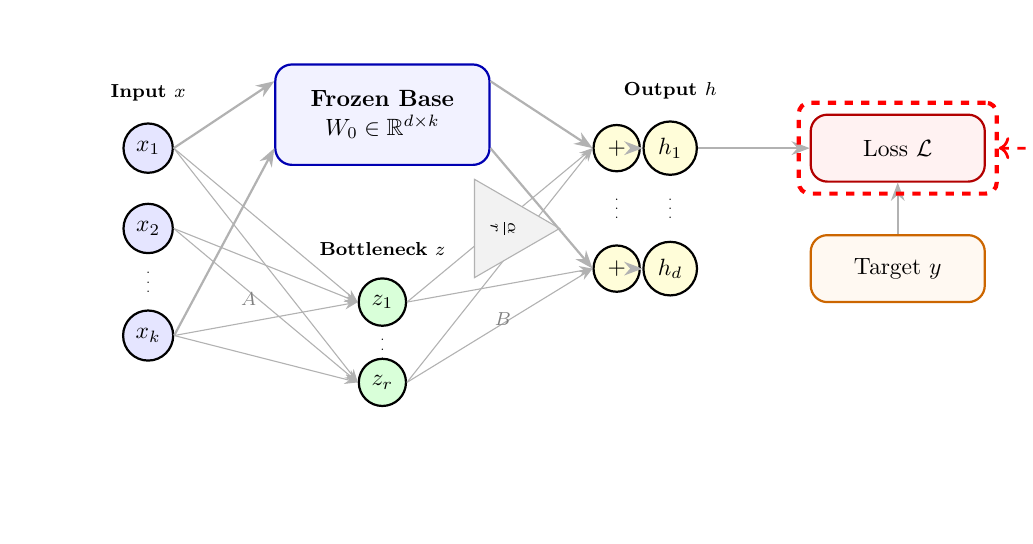
\begin{tikzpicture}[node distance=1.0cm and 1.5cm, scale=0.85, every node/.style={transform shape}]
  \useasboundingbox (-1.8, -3.5) rectangle (12.8, 3.8);
  % Input Neurons
  \node[neuron] (x1) at (0, 2) {$x_1$};
  \node[neuron] (x2) at (0, 0.8) {$x_2$};
  \node[neuron] (xk) at (0, -0.8) {$x_k$};
  \node[font=\tiny] at (0, 0.1) {$\vdots$};
  \node[lbl, above=0.2cm of x1] {Input $x$};

  % Base Weight Matrix W_0
  \node[frzblk, minimum width=3.2cm, minimum height=1.5cm] (W0) at (3.5, 2.5) {\textbf{Frozen Base} \\ $W_0 \in \mathbb{R}^{d \times k}$};

  % Bottleneck Neurons
  \node[bneck] (z1) at (3.5, -0.3) {$z_1$};
  \node[bneck] (zr) at (3.5, -1.5) {$z_r$};
  \node[font=\tiny] at (3.5, -0.9) {$\vdots$};
  \node[lbl, above=0.2cm of z1] {Bottleneck $z$};

  % Connections A
  \foreach \s in {x1,x2,xk} \foreach \t in {z1,zr}
    \draw[arr, gray!60, thin] (\s.east)--(\t.west);
  \node[text=gray, font=\footnotesize] at (1.5, -0.25) {$A$};

  % Summing Junctions and Output Neurons
  \node[sumnode] (sum1) at (7.0, 2) {$+$};
  \node[sumnode] (sumd) at (7.0, 0.2) {$+$};
  \node[font=\tiny] at (7.0, 1.2) {$\vdots$};
  
  \node[outnrn] (h1) at (7.8, 2) {$h_1$};
  \node[outnrn] (hd) at (7.8, 0.2) {$h_d$};
  \node[font=\tiny] at (7.8, 1.2) {$\vdots$};
  \node[lbl, above=0.2cm of h1] {Output $h$};

  % Connections B
  \foreach \s in {z1,zr} \foreach \t in {sum1,sumd}
    \draw[arr, gray!60, thin] (\s.east)--(\t.west);
  \node[text=gray, font=\footnotesize] at (5.3, -0.55) {$B$};

  % Scaling Multiplier
  \node[draw, regular polygon, regular polygon sides=3, rotate=-90, fill=gray!10, minimum size=0.9cm, draw=gray!60] (scale) at (5.3, 0.8) {$\frac{\alpha}{r}$};

  % Forward path connections
  \draw[arr, gray!60] (x1.east) -- ($(W0.west)+(0,0.5)$);
  \draw[arr, gray!60] (xk.east) -- ($(W0.west)+(0,-0.5)$);
  \draw[arr, gray!60] ($(W0.east)+(0,0.5)$) -- (sum1.west);
  \draw[arr, gray!60] ($(W0.east)+(0,-0.5)$) -- (sumd.west);
  \draw[arr, gray!60] (sum1) -- (h1);
  \draw[arr, gray!60] (sumd) -- (hd);

  % Loss and Target
  \node[datblk] (y) at (11.2, 0.2) {Target $y$};
  \node[lossblk] (loss) at (11.2, 2.0) {Loss $\mathcal{L}$};
  \draw[arr, gray!60] (h1.east) -- (loss.west);
  \draw[arr, gray!60] (y.north) -- (loss.south);
  
  % Dashed base outlines fit
  \node[fit=(x1) (x2) (xk)] (fit_x) {};
  \node[fit=(W0)] (fit_w0) {};
  \node[fit=(z1) (zr)] (fit_z) {};
  \node[fit=(sum1) (sumd) (h1) (hd)] (fit_h) {};

  \node[draw=red, dashed, rounded corners=4pt, fit=(loss), inner sep=4pt, line width=1.5pt] (circle_loss) {};
  \node[text=red, font=\bfseries\small, right=0.4cm of circle_loss, align=left] (lbl_loss) {HIGHLIGHT:\\Loss $\mathcal{L}$};
  \draw[dashed, red, line width=1pt, ->] (lbl_loss.west) -- (circle_loss.east);

\end{tikzpicture}
\end{adjustbox}
\vspace{1.5em}
\end{center}

      \item \textbf{Mental Model}: This is a single scorecard number. It tells us how far off the final output dials are from what they should be. If the score is high, it means the model is making bad guesses. The goal of training is to adjust the new dials until the scorecard reads zero.
      \item \textbf{Neuron-Level Physical Explanation}: The loss $\mathcal{L}$ measures how far the firing rates of the output neurons in the final layer differ from the desired target firing rates. The target represents the correct next word, and the error signal is generated by comparing the target with the actual outputs.
      \item \textbf{Mathematical Representation}: $\mathcal{L} \in \mathbb{R}$
      \item \textbf{Code Representation}: \texttt{loss = F.cross\_entropy(logits, targets)}
      \item \textbf{Relationships}: Traversed in reverse during backpropagation; all gradients are derivatives of $\mathcal{L}$.
    \end{itemize}

  \item \textbf{Output Layer Gradient ($\nabla_h \mathcal{L}$)}:
    \begin{itemize}
      \item \textbf{Formula}: $\nabla_h \mathcal{L} = \frac{\partial \mathcal{L}}{\partial h}$
      \item \textbf{Neuron Highlight Diagram}:

\begin{center}
\begin{adjustbox}{max width=0.85\linewidth}
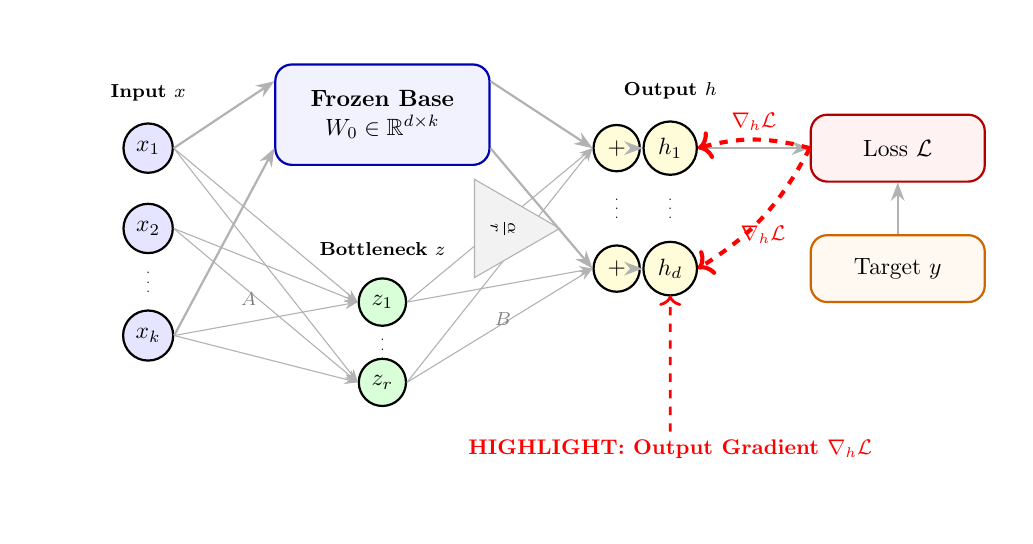
\begin{tikzpicture}[node distance=1.0cm and 1.5cm, scale=0.85, every node/.style={transform shape}]
  \useasboundingbox (-1.8, -3.5) rectangle (12.8, 3.8);
  % Input Neurons
  \node[neuron] (x1) at (0, 2) {$x_1$};
  \node[neuron] (x2) at (0, 0.8) {$x_2$};
  \node[neuron] (xk) at (0, -0.8) {$x_k$};
  \node[font=\tiny] at (0, 0.1) {$\vdots$};
  \node[lbl, above=0.2cm of x1] {Input $x$};

  % Base Weight Matrix W_0
  \node[frzblk, minimum width=3.2cm, minimum height=1.5cm] (W0) at (3.5, 2.5) {\textbf{Frozen Base} \\ $W_0 \in \mathbb{R}^{d \times k}$};

  % Bottleneck Neurons
  \node[bneck] (z1) at (3.5, -0.3) {$z_1$};
  \node[bneck] (zr) at (3.5, -1.5) {$z_r$};
  \node[font=\tiny] at (3.5, -0.9) {$\vdots$};
  \node[lbl, above=0.2cm of z1] {Bottleneck $z$};

  % Connections A
  \foreach \s in {x1,x2,xk} \foreach \t in {z1,zr}
    \draw[arr, gray!60, thin] (\s.east)--(\t.west);
  \node[text=gray, font=\footnotesize] at (1.5, -0.25) {$A$};

  % Summing Junctions and Output Neurons
  \node[sumnode] (sum1) at (7.0, 2) {$+$};
  \node[sumnode] (sumd) at (7.0, 0.2) {$+$};
  \node[font=\tiny] at (7.0, 1.2) {$\vdots$};
  
  \node[outnrn] (h1) at (7.8, 2) {$h_1$};
  \node[outnrn] (hd) at (7.8, 0.2) {$h_d$};
  \node[font=\tiny] at (7.8, 1.2) {$\vdots$};
  \node[lbl, above=0.2cm of h1] {Output $h$};

  % Connections B
  \foreach \s in {z1,zr} \foreach \t in {sum1,sumd}
    \draw[arr, gray!60, thin] (\s.east)--(\t.west);
  \node[text=gray, font=\footnotesize] at (5.3, -0.55) {$B$};

  % Scaling Multiplier
  \node[draw, regular polygon, regular polygon sides=3, rotate=-90, fill=gray!10, minimum size=0.9cm, draw=gray!60] (scale) at (5.3, 0.8) {$\frac{\alpha}{r}$};

  % Forward path connections
  \draw[arr, gray!60] (x1.east) -- ($(W0.west)+(0,0.5)$);
  \draw[arr, gray!60] (xk.east) -- ($(W0.west)+(0,-0.5)$);
  \draw[arr, gray!60] ($(W0.east)+(0,0.5)$) -- (sum1.west);
  \draw[arr, gray!60] ($(W0.east)+(0,-0.5)$) -- (sumd.west);
  \draw[arr, gray!60] (sum1) -- (h1);
  \draw[arr, gray!60] (sumd) -- (hd);

  % Loss and Target
  \node[datblk] (y) at (11.2, 0.2) {Target $y$};
  \node[lossblk] (loss) at (11.2, 2.0) {Loss $\mathcal{L}$};
  \draw[arr, gray!60] (h1.east) -- (loss.west);
  \draw[arr, gray!60] (y.north) -- (loss.south);
  
  % Dashed base outlines fit
  \node[fit=(x1) (x2) (xk)] (fit_x) {};
  \node[fit=(W0)] (fit_w0) {};
  \node[fit=(z1) (zr)] (fit_z) {};
  \node[fit=(sum1) (sumd) (h1) (hd)] (fit_h) {};

  \draw[arr, red, dashed, line width=1.5pt, ->] (loss.west) to[bend right=15] node[midway, above, red, font=\bfseries\small] {$\nabla_h \mathcal{L}$} (h1.east);
  \draw[arr, red, dashed, line width=1.5pt, ->] (loss.west) to[bend left=15] node[midway, below, red, font=\bfseries\small] {$\nabla_h \mathcal{L}$} (hd.east);
  \node[text=red, font=\bfseries\small] (lbl_gradh) at (7.8, -2.5) {HIGHLIGHT: Output Gradient $\nabla_h \mathcal{L}$};
  \draw[dashed, red, line width=1pt, ->] (lbl_gradh.north) -- (7.8, -0.2);

\end{tikzpicture}
\end{adjustbox}
\vspace{1.5em}
\end{center}

      \item \textbf{Mental Model}: This is a set of correction instructions for the final output dials. It says: "dial 1 needs to turn clockwise by $0.2$, and dial 2 needs to turn counter-clockwise by $1.5$" to lower the error score.
      \item \textbf{Neuron-Level Physical Explanation}: For a single output neuron $j$, the element $(\nabla_h \mathcal{L})_j = \frac{\partial \mathcal{L}}{\partial h_j}$ represents the error feedback signal. It tells the neuron whether it fired too strongly (positive gradient) or too weakly (negative gradient) and by how much it needs to adjust its total output to minimize the error.
      \item \textbf{Mathematical Representation}: $\nabla_h \mathcal{L} \in \mathbb{R}^{d \times 1}$
      \item \textbf{Code Representation}: automatically tracked by PyTorch's \texttt{loss.backward()}, represented as the grad tensor associated with output \texttt{h.grad}
      \item \textbf{Relationships}: Directly drives the gradient computation for $B$ and $z$.
    \end{itemize}

  \item \textbf{Bottleneck Layer Gradient ($\nabla_z \mathcal{L}$)}:
    \begin{itemize}
      \item \textbf{Formula}: $\nabla_z \mathcal{L} = \frac{\alpha}{r} B^\top \nabla_h \mathcal{L}$
      \item \textbf{Neuron Highlight Diagram}:

\begin{center}
\begin{adjustbox}{max width=0.85\linewidth}
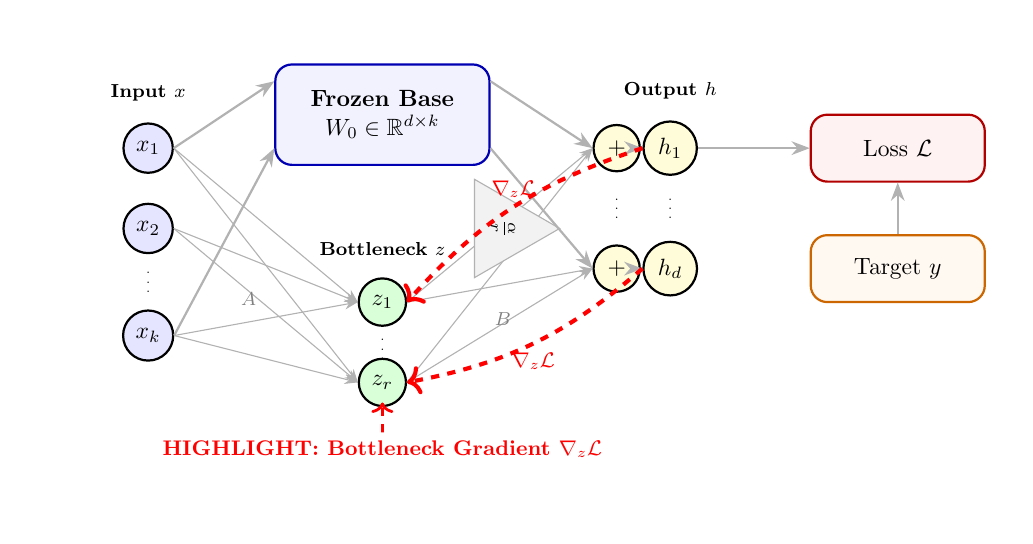
\begin{tikzpicture}[node distance=1.0cm and 1.5cm, scale=0.85, every node/.style={transform shape}]
  \useasboundingbox (-1.8, -3.5) rectangle (12.8, 3.8);
  % Input Neurons
  \node[neuron] (x1) at (0, 2) {$x_1$};
  \node[neuron] (x2) at (0, 0.8) {$x_2$};
  \node[neuron] (xk) at (0, -0.8) {$x_k$};
  \node[font=\tiny] at (0, 0.1) {$\vdots$};
  \node[lbl, above=0.2cm of x1] {Input $x$};

  % Base Weight Matrix W_0
  \node[frzblk, minimum width=3.2cm, minimum height=1.5cm] (W0) at (3.5, 2.5) {\textbf{Frozen Base} \\ $W_0 \in \mathbb{R}^{d \times k}$};

  % Bottleneck Neurons
  \node[bneck] (z1) at (3.5, -0.3) {$z_1$};
  \node[bneck] (zr) at (3.5, -1.5) {$z_r$};
  \node[font=\tiny] at (3.5, -0.9) {$\vdots$};
  \node[lbl, above=0.2cm of z1] {Bottleneck $z$};

  % Connections A
  \foreach \s in {x1,x2,xk} \foreach \t in {z1,zr}
    \draw[arr, gray!60, thin] (\s.east)--(\t.west);
  \node[text=gray, font=\footnotesize] at (1.5, -0.25) {$A$};

  % Summing Junctions and Output Neurons
  \node[sumnode] (sum1) at (7.0, 2) {$+$};
  \node[sumnode] (sumd) at (7.0, 0.2) {$+$};
  \node[font=\tiny] at (7.0, 1.2) {$\vdots$};
  
  \node[outnrn] (h1) at (7.8, 2) {$h_1$};
  \node[outnrn] (hd) at (7.8, 0.2) {$h_d$};
  \node[font=\tiny] at (7.8, 1.2) {$\vdots$};
  \node[lbl, above=0.2cm of h1] {Output $h$};

  % Connections B
  \foreach \s in {z1,zr} \foreach \t in {sum1,sumd}
    \draw[arr, gray!60, thin] (\s.east)--(\t.west);
  \node[text=gray, font=\footnotesize] at (5.3, -0.55) {$B$};

  % Scaling Multiplier
  \node[draw, regular polygon, regular polygon sides=3, rotate=-90, fill=gray!10, minimum size=0.9cm, draw=gray!60] (scale) at (5.3, 0.8) {$\frac{\alpha}{r}$};

  % Forward path connections
  \draw[arr, gray!60] (x1.east) -- ($(W0.west)+(0,0.5)$);
  \draw[arr, gray!60] (xk.east) -- ($(W0.west)+(0,-0.5)$);
  \draw[arr, gray!60] ($(W0.east)+(0,0.5)$) -- (sum1.west);
  \draw[arr, gray!60] ($(W0.east)+(0,-0.5)$) -- (sumd.west);
  \draw[arr, gray!60] (sum1) -- (h1);
  \draw[arr, gray!60] (sumd) -- (hd);

  % Loss and Target
  \node[datblk] (y) at (11.2, 0.2) {Target $y$};
  \node[lossblk] (loss) at (11.2, 2.0) {Loss $\mathcal{L}$};
  \draw[arr, gray!60] (h1.east) -- (loss.west);
  \draw[arr, gray!60] (y.north) -- (loss.south);
  
  % Dashed base outlines fit
  \node[fit=(x1) (x2) (xk)] (fit_x) {};
  \node[fit=(W0)] (fit_w0) {};
  \node[fit=(z1) (zr)] (fit_z) {};
  \node[fit=(sum1) (sumd) (h1) (hd)] (fit_h) {};

  \draw[arr, red, dashed, line width=1.5pt, ->] (h1.west) to[bend right=15] node[midway, above, red, font=\bfseries\small] {$\nabla_z \mathcal{L}$} (z1.east);
  \draw[arr, red, dashed, line width=1.5pt, ->] (hd.west) to[bend left=15] node[midway, below, red, font=\bfseries\small] {$\nabla_z \mathcal{L}$} (zr.east);
  \node[text=red, font=\bfseries\small] (lbl_gradz) at (3.5, -2.5) {HIGHLIGHT: Bottleneck Gradient $\nabla_z \mathcal{L}$};
  \draw[dashed, red, line width=1pt, ->] (lbl_gradz.north) -- (3.5, -1.8);

\end{tikzpicture}
\end{adjustbox}
\vspace{1.5em}
\end{center}

      \item \textbf{Mental Model}: This translates the correction instructions from the output room back down into the bottleneck. It tells the summary dials inside the funnel how they need to adjust to fix the output dials.
      \item \textbf{Neuron-Level Physical Explanation}: For a bottleneck neuron $m$, this is the backpropagated error signal. It is computed by summing the error feedback signals from all output neurons, weighted by their connections $B_{jm}$ and scaled: $(\nabla_z \mathcal{L})_m = \frac{\alpha}{r} \sum_j B_{jm} (\nabla_h \mathcal{L})_j$. It tells the bottleneck neuron how its activation should have changed.
      \item \textbf{Mathematical Representation}: $\nabla_z \mathcal{L} \in \mathbb{R}^{r \times 1}$
      \item \textbf{Code Representation}: \texttt{grad\_z = (alpha / r) * torch.matmul(grad\_output, B.weight)}
      \item \textbf{Relationships}: Drives the gradient computation for $A$.
    \end{itemize}

  \item \textbf{Update Gradient for Matrix $B$ ($\nabla_B \mathcal{L}$)}:
    \begin{itemize}
      \item \textbf{Formula}: $\nabla_B \mathcal{L} = \frac{\alpha}{r} (\nabla_h \mathcal{L}) z^\top$
      \item \textbf{Neuron Highlight Diagram}:

\begin{center}
\begin{adjustbox}{max width=0.85\linewidth}
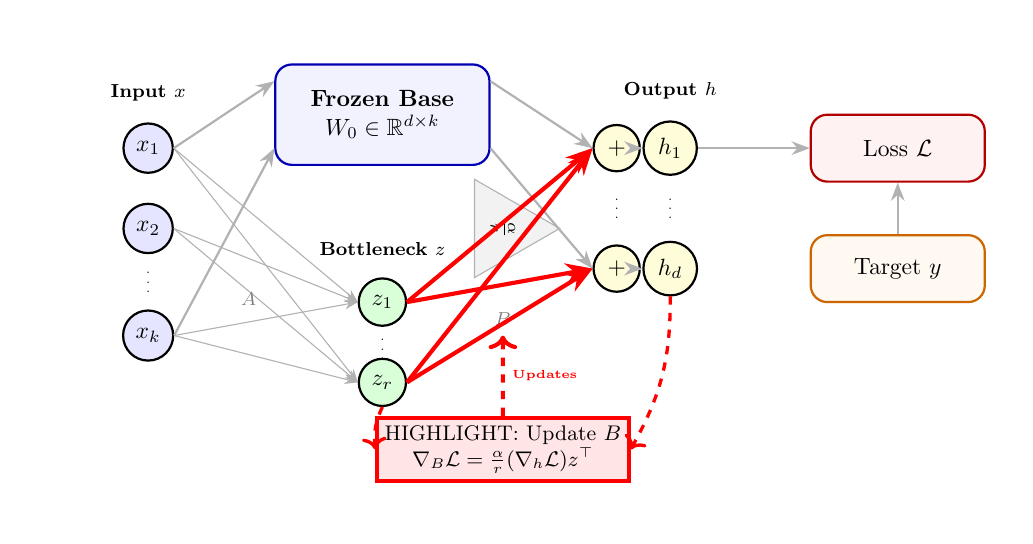
\begin{tikzpicture}[node distance=1.0cm and 1.5cm, scale=0.85, every node/.style={transform shape}]
  \useasboundingbox (-1.8, -3.5) rectangle (12.8, 3.8);
  % Input Neurons
  \node[neuron] (x1) at (0, 2) {$x_1$};
  \node[neuron] (x2) at (0, 0.8) {$x_2$};
  \node[neuron] (xk) at (0, -0.8) {$x_k$};
  \node[font=\tiny] at (0, 0.1) {$\vdots$};
  \node[lbl, above=0.2cm of x1] {Input $x$};

  % Base Weight Matrix W_0
  \node[frzblk, minimum width=3.2cm, minimum height=1.5cm] (W0) at (3.5, 2.5) {\textbf{Frozen Base} \\ $W_0 \in \mathbb{R}^{d \times k}$};

  % Bottleneck Neurons
  \node[bneck] (z1) at (3.5, -0.3) {$z_1$};
  \node[bneck] (zr) at (3.5, -1.5) {$z_r$};
  \node[font=\tiny] at (3.5, -0.9) {$\vdots$};
  \node[lbl, above=0.2cm of z1] {Bottleneck $z$};

  % Connections A
  \foreach \s in {x1,x2,xk} \foreach \t in {z1,zr}
    \draw[arr, gray!60, thin] (\s.east)--(\t.west);
  \node[text=gray, font=\footnotesize] at (1.5, -0.25) {$A$};

  % Summing Junctions and Output Neurons
  \node[sumnode] (sum1) at (7.0, 2) {$+$};
  \node[sumnode] (sumd) at (7.0, 0.2) {$+$};
  \node[font=\tiny] at (7.0, 1.2) {$\vdots$};
  
  \node[outnrn] (h1) at (7.8, 2) {$h_1$};
  \node[outnrn] (hd) at (7.8, 0.2) {$h_d$};
  \node[font=\tiny] at (7.8, 1.2) {$\vdots$};
  \node[lbl, above=0.2cm of h1] {Output $h$};

  % Connections B
  \foreach \s in {z1,zr} \foreach \t in {sum1,sumd}
    \draw[arr, gray!60, thin] (\s.east)--(\t.west);
  \node[text=gray, font=\footnotesize] at (5.3, -0.55) {$B$};

  % Scaling Multiplier
  \node[draw, regular polygon, regular polygon sides=3, rotate=-90, fill=gray!10, minimum size=0.9cm, draw=gray!60] (scale) at (5.3, 0.8) {$\frac{\alpha}{r}$};

  % Forward path connections
  \draw[arr, gray!60] (x1.east) -- ($(W0.west)+(0,0.5)$);
  \draw[arr, gray!60] (xk.east) -- ($(W0.west)+(0,-0.5)$);
  \draw[arr, gray!60] ($(W0.east)+(0,0.5)$) -- (sum1.west);
  \draw[arr, gray!60] ($(W0.east)+(0,-0.5)$) -- (sumd.west);
  \draw[arr, gray!60] (sum1) -- (h1);
  \draw[arr, gray!60] (sumd) -- (hd);

  % Loss and Target
  \node[datblk] (y) at (11.2, 0.2) {Target $y$};
  \node[lossblk] (loss) at (11.2, 2.0) {Loss $\mathcal{L}$};
  \draw[arr, gray!60] (h1.east) -- (loss.west);
  \draw[arr, gray!60] (y.north) -- (loss.south);
  
  % Dashed base outlines fit
  \node[fit=(x1) (x2) (xk)] (fit_x) {};
  \node[fit=(W0)] (fit_w0) {};
  \node[fit=(z1) (zr)] (fit_z) {};
  \node[fit=(sum1) (sumd) (h1) (hd)] (fit_h) {};

  \foreach \s in {z1,zr} \foreach \t in {sum1,sumd}
    \draw[arr, red, line width=1.5pt] (\s.east)--(\t.west);
  \node[draw=red, rectangle, fill=red!10, line width=1.5pt, font=\small, align=center] (gradB) at (5.3, -2.5) {HIGHLIGHT: Update $B$ \\ $\nabla_B \mathcal{L} = \frac{\alpha}{r} (\nabla_h \mathcal{L}) z^\top$};
  \draw[dashed, red, line width=1.2pt, ->] (zr.south) to[bend right=15] (gradB.west);
  \draw[dashed, red, line width=1.2pt, ->] (hd.south) to[bend left=15] (gradB.east);
  \draw[dashed, red, line width=1.5pt, ->] (gradB.north) -- (5.3, -0.8) node[midway, right, red, font=\bfseries\tiny] {Updates};

\end{tikzpicture}
\end{adjustbox}
\vspace{1.5em}
\end{center}

      \item \textbf{Mental Model}: This is the instruction sheet showing how to rewire the dials of the expansion nozzle ($B$) so that they do a better job of translating the summary back to the output dials.
      \item \textbf{Neuron-Level Physical Explanation}: For the synapse connecting bottleneck neuron $m$ to output neuron $j$, the gradient is calculated as $(\nabla_B \mathcal{L})_{jm} = \frac{\alpha}{r} (\nabla_h \mathcal{L})_j z_m$. This follows Hebbian learning: the strength of the update is proportional to the product of the pre-synaptic activation ($z_m$) and the post-synaptic error signal ($(\nabla_h \mathcal{L})_j$).
      \item \textbf{Mathematical Representation}: $\nabla_B \mathcal{L} \in \mathbb{R}^{d \times r}$
      \item \textbf{Code Representation}: \texttt{B.weight.grad = (alpha / r) * torch.matmul(grad\_output.t(), z)}
      \item \textbf{Relationships}: Used by the optimizer to update the values of $B$.
    \end{itemize}

  \item \textbf{Update Gradient for Matrix $A$ ($\nabla_A \mathcal{L}$)}:
    \begin{itemize}
      \item \textbf{Formula}: $\nabla_A \mathcal{L} = (\nabla_z \mathcal{L}) x^\top$
      \item \textbf{Neuron Highlight Diagram}:

\begin{center}
\begin{adjustbox}{max width=0.85\linewidth}
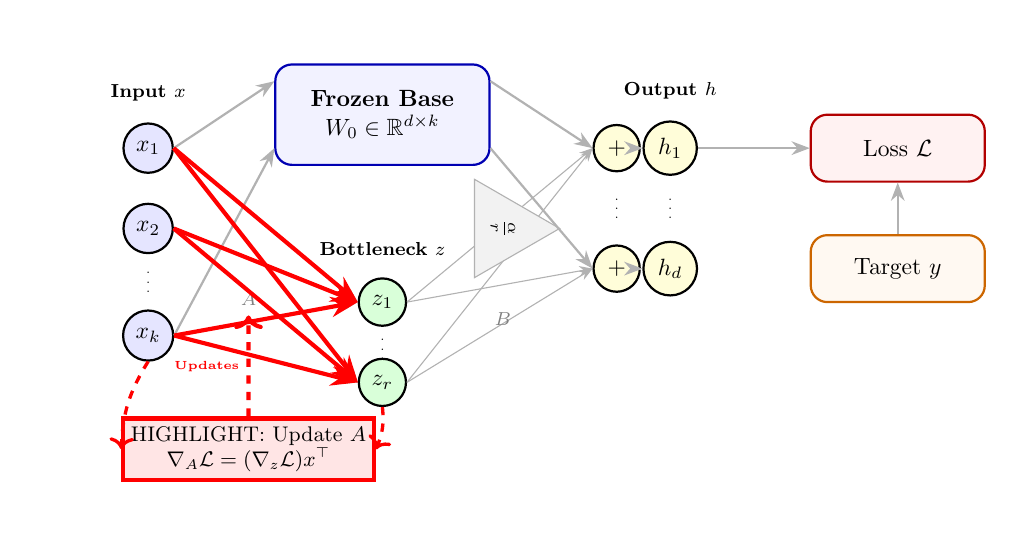
\begin{tikzpicture}[node distance=1.0cm and 1.5cm, scale=0.85, every node/.style={transform shape}]
  \useasboundingbox (-1.8, -3.5) rectangle (12.8, 3.8);
  % Input Neurons
  \node[neuron] (x1) at (0, 2) {$x_1$};
  \node[neuron] (x2) at (0, 0.8) {$x_2$};
  \node[neuron] (xk) at (0, -0.8) {$x_k$};
  \node[font=\tiny] at (0, 0.1) {$\vdots$};
  \node[lbl, above=0.2cm of x1] {Input $x$};

  % Base Weight Matrix W_0
  \node[frzblk, minimum width=3.2cm, minimum height=1.5cm] (W0) at (3.5, 2.5) {\textbf{Frozen Base} \\ $W_0 \in \mathbb{R}^{d \times k}$};

  % Bottleneck Neurons
  \node[bneck] (z1) at (3.5, -0.3) {$z_1$};
  \node[bneck] (zr) at (3.5, -1.5) {$z_r$};
  \node[font=\tiny] at (3.5, -0.9) {$\vdots$};
  \node[lbl, above=0.2cm of z1] {Bottleneck $z$};

  % Connections A
  \foreach \s in {x1,x2,xk} \foreach \t in {z1,zr}
    \draw[arr, gray!60, thin] (\s.east)--(\t.west);
  \node[text=gray, font=\footnotesize] at (1.5, -0.25) {$A$};

  % Summing Junctions and Output Neurons
  \node[sumnode] (sum1) at (7.0, 2) {$+$};
  \node[sumnode] (sumd) at (7.0, 0.2) {$+$};
  \node[font=\tiny] at (7.0, 1.2) {$\vdots$};
  
  \node[outnrn] (h1) at (7.8, 2) {$h_1$};
  \node[outnrn] (hd) at (7.8, 0.2) {$h_d$};
  \node[font=\tiny] at (7.8, 1.2) {$\vdots$};
  \node[lbl, above=0.2cm of h1] {Output $h$};

  % Connections B
  \foreach \s in {z1,zr} \foreach \t in {sum1,sumd}
    \draw[arr, gray!60, thin] (\s.east)--(\t.west);
  \node[text=gray, font=\footnotesize] at (5.3, -0.55) {$B$};

  % Scaling Multiplier
  \node[draw, regular polygon, regular polygon sides=3, rotate=-90, fill=gray!10, minimum size=0.9cm, draw=gray!60] (scale) at (5.3, 0.8) {$\frac{\alpha}{r}$};

  % Forward path connections
  \draw[arr, gray!60] (x1.east) -- ($(W0.west)+(0,0.5)$);
  \draw[arr, gray!60] (xk.east) -- ($(W0.west)+(0,-0.5)$);
  \draw[arr, gray!60] ($(W0.east)+(0,0.5)$) -- (sum1.west);
  \draw[arr, gray!60] ($(W0.east)+(0,-0.5)$) -- (sumd.west);
  \draw[arr, gray!60] (sum1) -- (h1);
  \draw[arr, gray!60] (sumd) -- (hd);

  % Loss and Target
  \node[datblk] (y) at (11.2, 0.2) {Target $y$};
  \node[lossblk] (loss) at (11.2, 2.0) {Loss $\mathcal{L}$};
  \draw[arr, gray!60] (h1.east) -- (loss.west);
  \draw[arr, gray!60] (y.north) -- (loss.south);
  
  % Dashed base outlines fit
  \node[fit=(x1) (x2) (xk)] (fit_x) {};
  \node[fit=(W0)] (fit_w0) {};
  \node[fit=(z1) (zr)] (fit_z) {};
  \node[fit=(sum1) (sumd) (h1) (hd)] (fit_h) {};

  \foreach \s in {x1,x2,xk} \foreach \t in {z1,zr}
    \draw[arr, red, line width=1.5pt] (\s.east)--(\t.west);
  \node[draw=red, rectangle, fill=red!10, line width=1.5pt, font=\small, align=center] (gradA) at (1.5, -2.5) {HIGHLIGHT: Update $A$ \\ $\nabla_A \mathcal{L} = (\nabla_z \mathcal{L}) x^\top$};
  \draw[dashed, red, line width=1.2pt, ->] (xk.south) to[bend right=15] (gradA.west);
  \draw[dashed, red, line width=1.2pt, ->] (zr.south) to[bend left=15] (gradA.east);
  \draw[dashed, red, line width=1.5pt, ->] (gradA.north) -- (1.5, -0.5) node[midway, left, red, font=\bfseries\tiny] {Updates};

\end{tikzpicture}
\end{adjustbox}
\vspace{1.5em}
\end{center}

      \item \textbf{Mental Model}: This is the instruction sheet showing how to rewire the dials of the compression funnel ($A$) so that they do a better job of compressing the input dials into the summary.
      \item \textbf{Neuron-Level Physical Explanation}: For the synapse connecting input neuron $i$ to bottleneck neuron $m$, the gradient is $(\nabla_A \mathcal{L})_{mi} = (\nabla_z \mathcal{L})_m x_i$. This also follows Hebbian learning: it multiplies the pre-synaptic input signal ($x_i$) by the post-synaptic bottleneck error signal ($(\nabla_z \mathcal{L})_m$) to determine how much the synapse should strengthen or weaken.
      \item \textbf{Mathematical Representation}: $\nabla_A \mathcal{L} \in \mathbb{R}^{r \times k}$
      \item \textbf{Code Representation}: \texttt{A.weight.grad = torch.matmul(grad\_z.t(), x)}
      \item \textbf{Relationships}: Used by the optimizer to update the values of $A$.
    \end{itemize}
\end{enumerate}

\section{The Physical and Philosophical Foundations of LoRA}

\subsection{Philosophical Foundations: Occam's Razor and the Manifold Hypothesis}
The success of Low-Rank Adaptation (LoRA) is not merely an empirical coincidence, but is deeply rooted in two foundational philosophical principles of complexity. We analyze each principle through a dialectic framework of Arguments, Counter-Arguments, and Rebuttals:

\paragraph{1. The Manifold Hypothesis}
\begin{itemize}
  \item \textbf{Argument}: This hypothesis posits that high-dimensional data (such as the activations in a neural network) actually lies on a much lower-dimensional, highly structured manifold. Pretraining constructs this manifold by mapping the topological structure of natural language.
  
  In the context of Large Language Models, the embedding space has an extrinsic dimension of k = 4096 (e.g., $d_{\text{model}} = 4096$). However, the set of all grammatically correct and semantically coherent sentences does not fill this space uniformly; instead, it is confined to a lower-dimensional manifold. When we adapt the model to a downstream task (e.g., teaching it Python syntax or chat style), we do not need to construct a new manifold. We only need to compute a small trajectory or translation vector along the existing surface. This translation vector corresponds to a tangent vector in the manifold's tangent bundle. By confining our search to this tangent space, we avoid distorting the global topology of the language manifold, preventing catastrophic forgetting.
  
  \item \textbf{Counter-Argument}: If the downstream task represents an extreme domain shift (e.g., shifting from English literature to highly specialized biochemistry nomenclature or low-level assembly code), the target representations may lie completely outside the manifold mapped during pretraining. In such cases, the translation vector cannot lie along the existing manifold surface, and restricting the updates to a low-rank tangent space will lead to underfitting. The model would fail to acquire the new features because the required coordinates do not exist in the pretrained column space.
  
  \item \textbf{Rebuttal / Synthesis}: While severe domain shifts can strain low-rank constraints, empirical evidence shows that even highly specialized knowledge maps back to general-purpose linguistic structures (syntax, logic, context). Furthermore, if the target lies slightly off-manifold, a small rank $r$ (e.g., 8 to 16) is still sufficient to project the input into the nearest point on the task manifold. If needed, the user can scale the rank $r$ to increase the degrees of freedom, which mathematically expands the coordinate projection space, allowing the model to capture features that lie slightly outside the pretraining manifold while still regularizing the update to prevent arbitrary drift.
\end{itemize}

\paragraph{2. Occam's Razor (Lex Parsimoniae)}
\begin{itemize}
  \item \textbf{Argument}: Plurality should not be posited without necessity. Full fine-tuning searches an extremely large, redundant parameter space ($\mathbb{R}^{d \times k}$), which contains millions of redundant degrees of freedom. This massive parameter space allows the model to find arbitrary, highly complex fitting functions that overfit the downstream training data and overwrite pretrained general knowledge.
  
  By restricting the learning search to a compressed subspace ($\mathbb{R}^{r \times (k+d)}$), LoRA acts as a mathematical regularization agent. It forces the model to find the simplest, most parsimonious path of adaptation. This acts as a geometric constraint (projection regularization), restricting updates to only the principal directions of adaptation, thereby preserving the model's core foundational capabilities.
  
  \item \textbf{Counter-Argument}: By restricting the parameters to a low-rank product $BA$, we might force the model to find an oversimplified adaptation path that fails to capture the subtle, non-linear correlations required for complex reasoning tasks. Furthermore, Occam's Razor assumes that simpler models generalize better, but in deep learning, the phenomenon of "double descent" shows that highly overparameterized models can generalize better than simpler ones by finding smooth interpolating functions in high-dimensional spaces.
  
  \item \textbf{Rebuttal / Synthesis}: Double descent occurs when the entire network is overparameterized and trained on vast, diverse datasets where it can interpolate smoothly. However, in downstream fine-tuning, the dataset is small and highly focused. In this regime, overparameterization leads to catastrophic forgetting and representation collapse. Constraining the updates to a low-rank subspace restricts the model from modifying the general-purpose features, while allowing sufficient capacity to learn the task. Thus, LoRA combines the benefits of high-dimensional pretraining (smooth interpolation on general data) with low-dimensional adaptation (strict regularization on task-specific data).
\end{itemize}

\subsection{Internal Mechanics and Representation Space Geometry}
To understand why LoRA works under the hood, we must analyze the geometry of representation space and the intrinsic dimension of neural networks:
\begin{itemize}
  \item \textbf{Intrinsic vs. Extrinsic Dimension}: A pretrained model has a very high extrinsic dimension (the number of weights $W_0 \in \mathbb{R}^{d \times k}$). However, empirical work by Aghajanyan et al. (2020) demonstrated that the parameter space of pretrained language models has a much lower \textit{intrinsic dimension}. That is, the directions in weight space that significantly affect the loss are highly concentrated on a low-dimensional subspace. This is why we can optimize a tiny fraction of parameters and achieve the same or better task performance.
  \item \textbf{Subspace Alignment and Trajectory Geometry}: The activation vectors $x$ represent coordinates on the manifold. The base weight matrix $W_0$ maps these coordinates to the next representation space. The update matrix $\Delta W = \frac{\alpha}{r} B A$ acts as a linear projection operator that projects the activations into a tiny subspace of dimension $r$ via $A$, rotates/scales them in this bottleneck space, and then projects them back to the output space via $B$. This operation restricts the adaptation to a set of $r$ directional vectors. Instead of shifting the entire coordinate frame, the adapter only redirects the activation trajectory along the principal directions relevant to the downstream task.
  
  Geometrically, the column space of $\Delta W$ is spanned by the columns of $B$, which is an $r$-dimensional subspace of the output space $\mathbb{R}^{d}$. The row space of $\Delta W$ is spanned by the rows of $A$, which is an $r$-dimensional subspace of the input space $\mathbb{R}^{k}$. Thus, the adaptation updates are strictly constrained to these coordinates, preserving all other dimensions from degradation.
\end{itemize}

\subsection{Visualizing the Calculations}
We can visualize how the information bottleneck constrains the updates in the representation space during the forward and backward passes:

\begin{figure}[h]
\centering
\begin{adjustbox}{max width=0.9\linewidth}
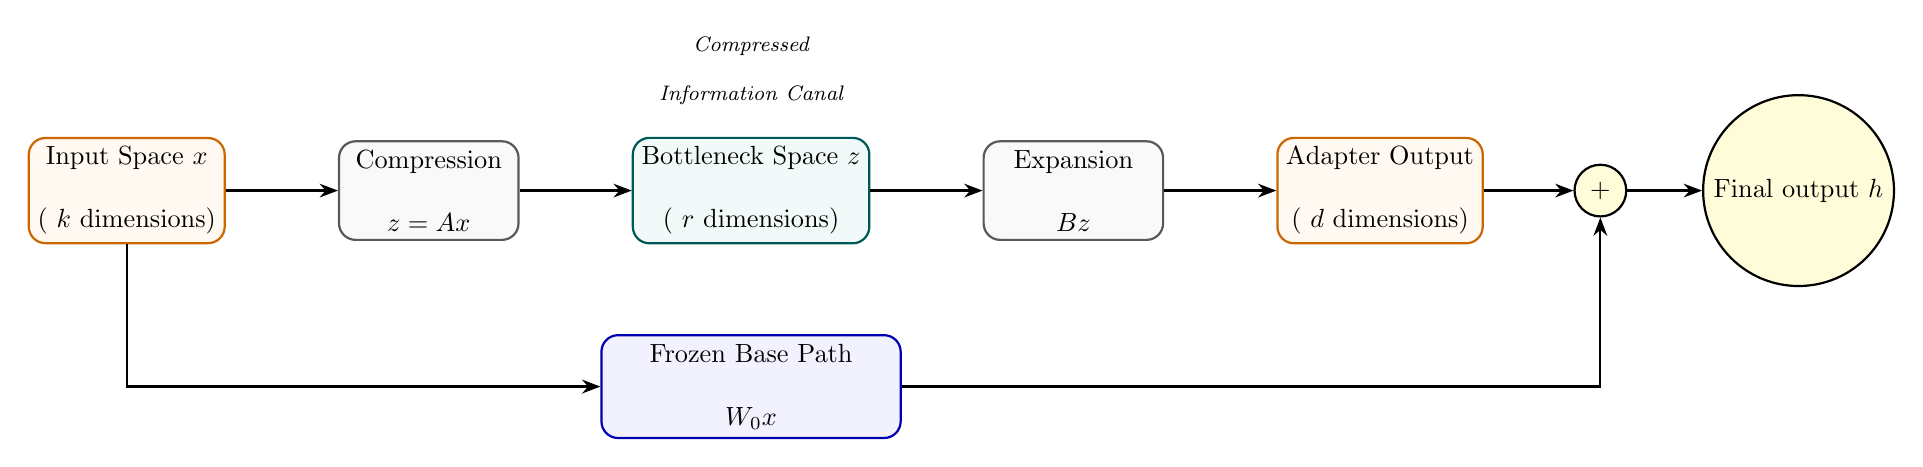
\begin{tikzpicture}[node distance=1.0cm and 1.5cm, scale=0.95, every node/.style={transform shape}]
  \node[datblk] (input) {Input Space $x$\\\\( $k$ dimensions)};
  \node[grayblk, right=of input, minimum width=2.4cm] (project) {Compression\\\\$z = Ax$};
  \node[trnblk, right=of project, minimum width=2.4cm] (bottleneck) {Bottleneck Space $z$\\\\( $r$ dimensions)};
  \node[grayblk, right=of bottleneck, minimum width=2.4cm] (expand) {Expansion\\\\$B z$};
  \node[datblk, right=of expand, minimum width=2.4cm] (out_lora) {Adapter Output\\\\( $d$ dimensions)};
  
  \node[frzblk, below=1.2cm of bottleneck, minimum width=4cm] (base) {Frozen Base Path\\\\$W_0 x$};
  \node[sumnode, right=1.2cm of out_lora] (sum) {$+$};
  \node[outnrn, right=1.0cm of sum] (output) {Final output $h$};

  \draw[arr] (input) -- (project);
  \draw[arr] (project) -- (bottleneck);
  \draw[arr] (bottleneck) -- (expand);
  \draw[arr] (expand) -- (out_lora);
  \draw[arr] (out_lora) -- (sum);
  \draw[arr] (sum) -- (output);
  
  \draw[arr] (input.south) |- (base.west);
  \draw[arr] (base.east) -| (sum.south);
  
  \node[font=\footnotesize\itshape, align=center, above=0.3cm of bottleneck] {Compressed\\\\Information Canal};
\end{tikzpicture}
\end{adjustbox}
\caption{Visualization of the information bottleneck: high-dimensional input is projected into a low-dimensional canal where task-specific tuning forces are applied, then projected back.}
\end{figure}

\begin{itemize}
  \item \textbf{Forward Pass Compression}: The activation vector $x \in \mathbb{R}^{k \times 1}$ is projected down through a narrow bottleneck of rank $r$. Since $r \ll \min(k, d)$, the projection filters out dimensions irrelevant to the current task, creating a compressed task representation $z \in \mathbb{R}^{r \times 1}$.
  \item \textbf{Backward Pass Gradient Flow}: Error gradients $\nabla_h \mathcal{L}$ flow backwards. Because $W_0$ is frozen and lacks a gradient buffer, no gradient update calculations occur on the base weight matrix. Instead, the gradients flow down the low-rank adapters $B$ and $A$, computing updates specifically for the low-rank subspace and avoiding parameter updates across the whole network.
\end{itemize}

\section{The Physical and Philosophical Foundations of LoRA}

\subsection{Philosophical Foundations: Occam's Razor and the Manifold Hypothesis}
The success of Low-Rank Adaptation (LoRA) is not merely an empirical coincidence, but is deeply rooted in two foundational philosophical principles of complexity. We analyze each principle through a dialectic framework of Arguments, Counter-Arguments, and Rebuttals:

\paragraph{1. The Manifold Hypothesis}
\begin{itemize}
  \item \textbf{Argument}: This hypothesis posits that high-dimensional data (such as the activations in a neural network) actually lies on a much lower-dimensional, highly structured manifold. Pretraining constructs this manifold by mapping the topological structure of natural language.
  
  In the context of Large Language Models, the embedding space has an extrinsic dimension of k = 4096 (e.g., $d_{\text{model}} = 4096$). However, the set of all grammatically correct and semantically coherent sentences does not fill this space uniformly; instead, it is confined to a lower-dimensional manifold. When we adapt the model to a downstream task (e.g., teaching it Python syntax or chat style), we do not need to construct a new manifold. We only need to compute a small trajectory or translation vector along the existing surface. This translation vector corresponds to a tangent vector in the manifold's tangent bundle. By confining our search to this tangent space, we avoid distorting the global topology of the language manifold, preventing catastrophic forgetting.
  
  \item \textbf{Counter-Argument}: If the downstream task represents an extreme domain shift (e.g., shifting from English literature to highly specialized biochemistry nomenclature or low-level assembly code), the target representations may lie completely outside the manifold mapped during pretraining. In such cases, the translation vector cannot lie along the existing manifold surface, and restricting the updates to a low-rank tangent space will lead to underfitting. The model would fail to acquire the new features because the required coordinates do not exist in the pretrained column space.
  
  \item \textbf{Rebuttal / Synthesis}: While severe domain shifts can strain low-rank constraints, empirical evidence shows that even highly specialized knowledge maps back to general-purpose linguistic structures (syntax, logic, context). Furthermore, if the target lies slightly off-manifold, a small rank $r$ (e.g., 8 to 16) is still sufficient to project the input into the nearest point on the task manifold. If needed, the user can scale the rank $r$ to increase the degrees of freedom, which mathematically expands the coordinate projection space, allowing the model to capture features that lie slightly outside the pretraining manifold while still regularizing the update to prevent arbitrary drift.
\end{itemize}

\paragraph{2. Occam's Razor (Lex Parsimoniae)}
\begin{itemize}
  \item \textbf{Argument}: Plurality should not be posited without necessity. Full fine-tuning searches an extremely large, redundant parameter space ($\mathbb{R}^{d \times k}$), which contains millions of redundant degrees of freedom. This massive parameter space allows the model to find arbitrary, highly complex fitting functions that overfit the downstream training data and overwrite pretrained general knowledge.
  
  By restricting the learning search to a compressed subspace ($\mathbb{R}^{r \times (k+d)}$), LoRA acts as a mathematical regularization agent. It forces the model to find the simplest, most parsimonious path of adaptation. This acts as a geometric constraint (projection regularization), restricting updates to only the principal directions of adaptation, thereby preserving the model's core foundational capabilities.
  
  \item \textbf{Counter-Argument}: By restricting the parameters to a low-rank product $BA$, we might force the model to find an oversimplified adaptation path that fails to capture the subtle, non-linear correlations required for complex reasoning tasks. Furthermore, Occam's Razor assumes that simpler models generalize better, but in deep learning, the phenomenon of "double descent" shows that highly overparameterized models can generalize better than simpler ones by finding smooth interpolating functions in high-dimensional spaces.
  
  \item \textbf{Rebuttal / Synthesis}: Double descent occurs when the entire network is overparameterized and trained on vast, diverse datasets where it can interpolate smoothly. However, in downstream fine-tuning, the dataset is small and highly focused. In this regime, overparameterization leads to catastrophic forgetting and representation collapse. Constraining the updates to a low-rank subspace restricts the model from modifying the general-purpose features, while allowing sufficient capacity to learn the task. Thus, LoRA combines the benefits of high-dimensional pretraining (smooth interpolation on general data) with low-dimensional adaptation (strict regularization on task-specific data).
\end{itemize}

\subsection{Internal Mechanics and Representation Space Geometry}
To understand why LoRA works under the hood, we must analyze the geometry of representation space and the intrinsic dimension of neural networks:
\begin{itemize}
  \item \textbf{Intrinsic vs. Extrinsic Dimension}: A pretrained model has a very high extrinsic dimension (the number of weights $W_0 \in \mathbb{R}^{d \times k}$). However, empirical work by Aghajanyan et al. (2020) demonstrated that the parameter space of pretrained language models has a much lower \textit{intrinsic dimension}. That is, the directions in weight space that significantly affect the loss are highly concentrated on a low-dimensional subspace. This is why we can optimize a tiny fraction of parameters and achieve the same or better task performance.
  \item \textbf{Subspace Alignment and Trajectory Geometry}: The activation vectors $x$ represent coordinates on the manifold. The base weight matrix $W_0$ maps these coordinates to the next representation space. The update matrix $\Delta W = \frac{\alpha}{r} B A$ acts as a linear projection operator that projects the activations into a tiny subspace of dimension $r$ via $A$, rotates/scales them in this bottleneck space, and then projects them back to the output space via $B$. This operation restricts the adaptation to a set of $r$ directional vectors. Instead of shifting the entire coordinate frame, the adapter only redirects the activation trajectory along the principal directions relevant to the downstream task.
  
  Geometrically, the column space of $\Delta W$ is spanned by the columns of $B$, which is an $r$-dimensional subspace of the output space $\mathbb{R}^{d}$. The row space of $\Delta W$ is spanned by the rows of $A$, which is an $r$-dimensional subspace of the input space $\mathbb{R}^{k}$. Thus, the adaptation updates are strictly constrained to these coordinates, preserving all other dimensions from degradation.
\end{itemize}

\subsection{Visualizing the Calculations}
We can visualize how the information bottleneck constrains the updates in the representation space during the forward and backward passes:

\begin{figure}[h]
\centering
\begin{adjustbox}{max width=0.9\linewidth}
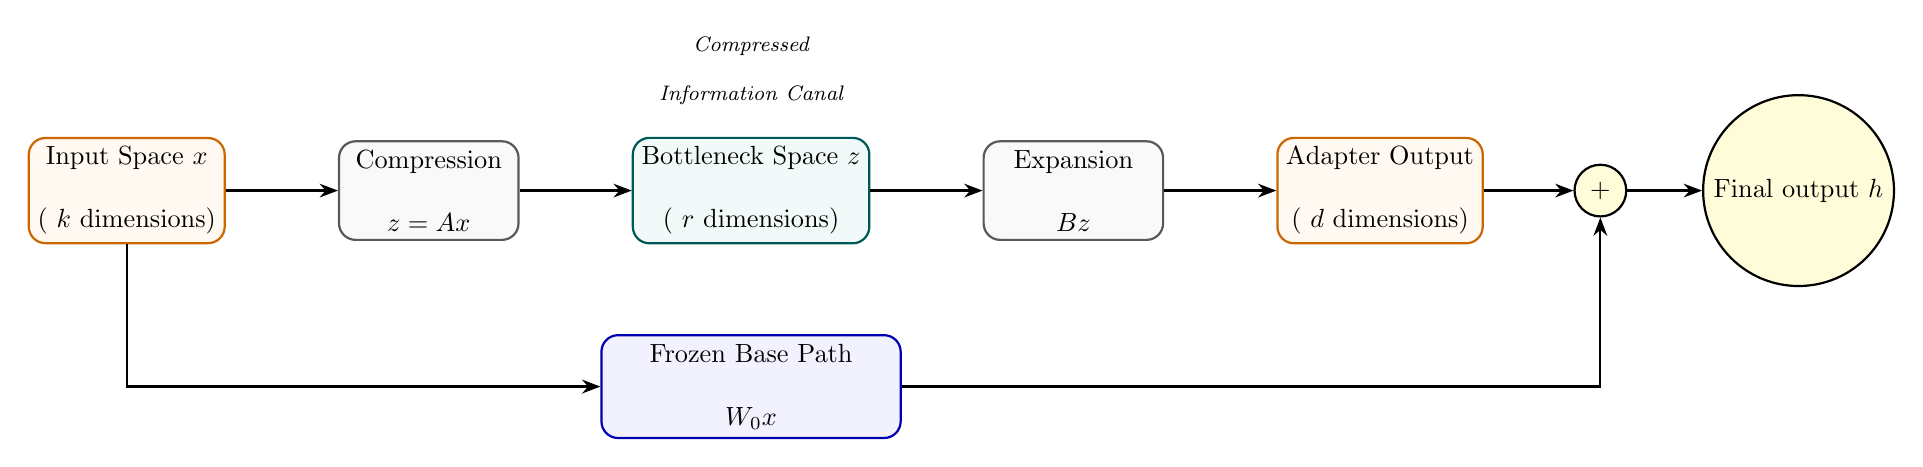
\begin{tikzpicture}[node distance=1.0cm and 1.5cm, scale=0.95, every node/.style={transform shape}]
  \node[datblk] (input) {Input Space $x$\\\\( $k$ dimensions)};
  \node[grayblk, right=of input, minimum width=2.4cm] (project) {Compression\\\\$z = Ax$};
  \node[trnblk, right=of project, minimum width=2.4cm] (bottleneck) {Bottleneck Space $z$\\\\( $r$ dimensions)};
  \node[grayblk, right=of bottleneck, minimum width=2.4cm] (expand) {Expansion\\\\$B z$};
  \node[datblk, right=of expand, minimum width=2.4cm] (out_lora) {Adapter Output\\\\( $d$ dimensions)};
  
  \node[frzblk, below=1.2cm of bottleneck, minimum width=4cm] (base) {Frozen Base Path\\\\$W_0 x$};
  \node[sumnode, right=1.2cm of out_lora] (sum) {$+$};
  \node[outnrn, right=1.0cm of sum] (output) {Final output $h$};

  \draw[arr] (input) -- (project);
  \draw[arr] (project) -- (bottleneck);
  \draw[arr] (bottleneck) -- (expand);
  \draw[arr] (expand) -- (out_lora);
  \draw[arr] (out_lora) -- (sum);
  \draw[arr] (sum) -- (output);
  
  \draw[arr] (input.south) |- (base.west);
  \draw[arr] (base.east) -| (sum.south);
  
  \node[font=\footnotesize\itshape, align=center, above=0.3cm of bottleneck] {Compressed\\\\Information Canal};
\end{tikzpicture}
\end{adjustbox}
\caption{Visualization of the information bottleneck: high-dimensional input is projected into a low-dimensional canal where task-specific tuning forces are applied, then projected back.}
\end{figure}

\begin{itemize}
  \item \textbf{Forward Pass Compression}: The activation vector $x \in \mathbb{R}^{k \times 1}$ is projected down through a narrow bottleneck of rank $r$. Since $r \ll \min(k, d)$, the projection filters out dimensions irrelevant to the current task, creating a compressed task representation $z \in \mathbb{R}^{r \times 1}$.
  \item \textbf{Backward Pass Gradient Flow}: Error gradients $\nabla_h \mathcal{L}$ flow backwards. Because $W_0$ is frozen and lacks a gradient buffer, no gradient update calculations occur on the base weight matrix. Instead, the gradients flow down the low-rank adapters $B$ and $A$, computing updates specifically for the low-rank subspace and avoiding parameter updates across the whole network.
\end{itemize}

\section{The Physical and Philosophical Foundations of LoRA}

\subsection{Philosophical Foundations: Occam's Razor and the Manifold Hypothesis}
The success of Low-Rank Adaptation (LoRA) is not merely an empirical coincidence, but is deeply rooted in two foundational philosophical principles of complexity. We analyze each principle through a dialectic framework of Arguments, Counter-Arguments, and Rebuttals:

\paragraph{1. The Manifold Hypothesis}
\begin{itemize}
  \item \textbf{Argument}: This hypothesis posits that high-dimensional data (such as the activations in a neural network) actually lies on a much lower-dimensional, highly structured manifold. Pretraining constructs this manifold by mapping the topological structure of natural language.
  
  In the context of Large Language Models, the embedding space has an extrinsic dimension of k = 4096 (e.g., $d_{\text{model}} = 4096$). However, the set of all grammatically correct and semantically coherent sentences does not fill this space uniformly; instead, it is confined to a lower-dimensional manifold. When we adapt the model to a downstream task (e.g., teaching it Python syntax or chat style), we do not need to construct a new manifold. We only need to compute a small trajectory or translation vector along the existing surface. This translation vector corresponds to a tangent vector in the manifold's tangent bundle. By confining our search to this tangent space, we avoid distorting the global topology of the language manifold, preventing catastrophic forgetting.
  
  \item \textbf{Counter-Argument}: If the downstream task represents an extreme domain shift (e.g., shifting from English literature to highly specialized biochemistry nomenclature or low-level assembly code), the target representations may lie completely outside the manifold mapped during pretraining. In such cases, the translation vector cannot lie along the existing manifold surface, and restricting the updates to a low-rank tangent space will lead to underfitting. The model would fail to acquire the new features because the required coordinates do not exist in the pretrained column space.
  
  \item \textbf{Rebuttal / Synthesis}: While severe domain shifts can strain low-rank constraints, empirical evidence shows that even highly specialized knowledge maps back to general-purpose linguistic structures (syntax, logic, context). Furthermore, if the target lies slightly off-manifold, a small rank $r$ (e.g., 8 to 16) is still sufficient to project the input into the nearest point on the task manifold. If needed, the user can scale the rank $r$ to increase the degrees of freedom, which mathematically expands the coordinate projection space, allowing the model to capture features that lie slightly outside the pretraining manifold while still regularizing the update to prevent arbitrary drift.
\end{itemize}

\paragraph{2. Occam's Razor (Lex Parsimoniae)}
\begin{itemize}
  \item \textbf{Argument}: Plurality should not be posited without necessity. Full fine-tuning searches an extremely large, redundant parameter space ($\mathbb{R}^{d \times k}$), which contains millions of redundant degrees of freedom. This massive parameter space allows the model to find arbitrary, highly complex fitting functions that overfit the downstream training data and overwrite pretrained general knowledge.
  
  By restricting the learning search to a compressed subspace ($\\mathbb{R}^{r \\times (k+d)}$), LoRA acts as a mathematical regularization agent. It forces the model to find the simplest, most parsimonious path of adaptation. This acts as a geometric constraint (projection regularization), restricting updates to only the principal directions of adaptation, thereby preserving the model's core foundational capabilities.
  
  \item \textbf{Counter-Argument}: By restricting the parameters to a low-rank product $BA$, we might force the model to find an oversimplified adaptation path that fails to capture the subtle, non-linear correlations required for complex reasoning tasks. Furthermore, Occam's Razor assumes that simpler models generalize better, but in deep learning, the phenomenon of "double descent" shows that highly overparameterized models can generalize better than simpler ones by finding smooth interpolating functions in high-dimensional spaces.
  
  \item \textbf{Rebuttal / Synthesis}: Double descent occurs when the entire network is overparameterized and trained on vast, diverse datasets where it can interpolate smoothly. However, in downstream fine-tuning, the dataset is small and highly focused. In this regime, overparameterization leads to catastrophic forgetting and representation collapse. Constraining the updates to a low-rank subspace restricts the model from modifying the general-purpose features, while allowing sufficient capacity to learn the task. Thus, LoRA combines the benefits of high-dimensional pretraining (smooth interpolation on general data) with low-dimensional adaptation (strict regularization on task-specific data).
\end{itemize}

\subsection{Internal Mechanics and Representation Space Geometry}
To understand why LoRA works under the hood, we must analyze the geometry of representation space and the intrinsic dimension of neural networks:
\begin{itemize}
  \item \textbf{Intrinsic vs. Extrinsic Dimension}: A pretrained model has a very high extrinsic dimension (the number of weights $W_0 \in \mathbb{R}^{d \times k}$). However, empirical work by Aghajanyan et al. (2020) demonstrated that the parameter space of pretrained language models has a much lower \textit{intrinsic dimension}. That is, the directions in weight space that significantly affect the loss are highly concentrated on a low-dimensional subspace. This is why we can optimize a tiny fraction of parameters and achieve the same or better task performance.
  \item \textbf{Subspace Alignment and Trajectory Geometry}: The activation vectors $x$ represent coordinates on the manifold. The base weight matrix $W_0$ maps these coordinates to the next representation space. The update matrix $\Delta W = \frac{\alpha}{r} B A$ acts as a linear projection operator that projects the activations into a tiny subspace of dimension $r$ via $A$, rotates/scales them in this bottleneck space, and then projects them back to the output space via $B$. This operation restricts the adaptation to a set of $r$ directional vectors. Instead of shifting the entire coordinate frame, the adapter only redirects the activation trajectory along the principal directions relevant to the downstream task.
  
  Geometrically, the column space of $\Delta W$ is spanned by the columns of $B$, which is an $r$-dimensional subspace of the output space $\mathbb{R}^{d}$. The row space of $\Delta W$ is spanned by the rows of $A$, which is an $r$-dimensional subspace of the input space $\mathbb{R}^{k}$. Thus, the adaptation updates are strictly constrained to these coordinates, preserving all other dimensions from degradation.
\end{itemize}

\subsection{Visualizing the Calculations}
We can visualize how the information bottleneck constrains the updates in the representation space during the forward and backward passes:

\begin{figure}[h]
\centering
\begin{adjustbox}{max width=0.9\linewidth}
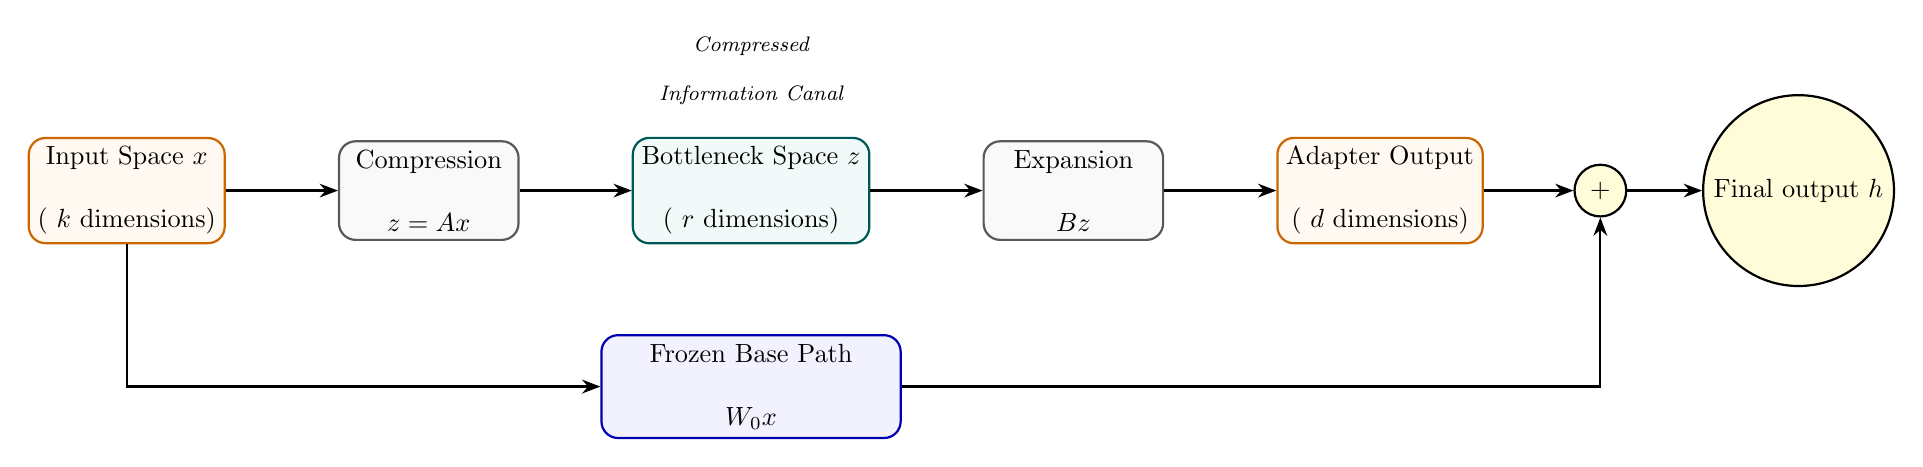
\begin{tikzpicture}[node distance=1.0cm and 1.5cm, scale=0.95, every node/.style={transform shape}]
  \node[datblk] (input) {Input Space $x$\\\\( $k$ dimensions)};
  \node[grayblk, right=of input, minimum width=2.4cm] (project) {Compression\\\\$z = Ax$};
  \node[trnblk, right=of project, minimum width=2.4cm] (bottleneck) {Bottleneck Space $z$\\\\( $r$ dimensions)};
  \node[grayblk, right=of bottleneck, minimum width=2.4cm] (expand) {Expansion\\\\$B z$};
  \node[datblk, right=of expand, minimum width=2.4cm] (out_lora) {Adapter Output\\\\( $d$ dimensions)};
  
  \node[frzblk, below=1.2cm of bottleneck, minimum width=4cm] (base) {Frozen Base Path\\\\$W_0 x$};
  \node[sumnode, right=1.2cm of out_lora] (sum) {$+$};
  \node[outnrn, right=1.0cm of sum] (output) {Final output $h$};

  \draw[arr] (input) -- (project);
  \draw[arr] (project) -- (bottleneck);
  \draw[arr] (bottleneck) -- (expand);
  \draw[arr] (expand) -- (out_lora);
  \draw[arr] (out_lora) -- (sum);
  \draw[arr] (sum) -- (output);
  
  \draw[arr] (input.south) |- (base.west);
  \draw[arr] (base.east) -| (sum.south);
  
  \node[font=\footnotesize\itshape, align=center, above=0.3cm of bottleneck] {Compressed\\\\Information Canal};
\end{tikzpicture}
\end{adjustbox}
\caption{Visualization of the information bottleneck: high-dimensional input is projected into a low-dimensional canal where task-specific tuning forces are applied, then projected back.}
\end{figure}

\begin{itemize}
  \item \textbf{Forward Pass Compression}: The activation vector $x \in \mathbb{R}^{k \times 1}$ is projected down through a narrow bottleneck of rank $r$. Since $r \ll \min(k, d)$, the projection filters out dimensions irrelevant to the current task, creating a compressed task representation $z \in \mathbb{R}^{r \times 1}$.
  \item \textbf{Backward Pass Gradient Flow}: Error gradients $\nabla_h \mathcal{L}$ flow backwards. Because $W_0$ is frozen and lacks a gradient buffer, no gradient update calculations occur on the base weight matrix. Instead, the gradients flow down the low-rank adapters $B$ and $A$, computing updates specifically for the low-rank subspace and avoiding parameter updates across the whole network.
\end{itemize}

\section{The Physical and Philosophical Foundations of LoRA}

\subsection{Philosophical Foundations: Occam's Razor and the Manifold Hypothesis}
The success of Low-Rank Adaptation (LoRA) is not merely an empirical coincidence, but is deeply rooted in two foundational philosophical principles of complexity. We analyze each principle through a dialectic framework of Arguments, Counter-Arguments, and Rebuttals:

\paragraph{1. The Manifold Hypothesis}
\begin{itemize}
  \item \textbf{Argument}: This hypothesis posits that high-dimensional data (such as the activations in a neural network) actually lies on a much lower-dimensional, highly structured manifold. Pretraining constructs this manifold by mapping the topological structure of natural language.
  
  In the context of Large Language Models, the embedding space has an extrinsic dimension of k = 4096 (e.g., $d_{\text{model}} = 4096$). However, the set of all grammatically correct and semantically coherent sentences does not fill this space uniformly; instead, it is confined to a lower-dimensional manifold. When we adapt the model to a downstream task (e.g., teaching it Python syntax or chat style), we do not need to construct a new manifold. We only need to compute a small trajectory or translation vector along the existing surface. This translation vector corresponds to a tangent vector in the manifold's tangent bundle. By confining our search to this tangent space, we avoid distorting the global topology of the language manifold, preventing catastrophic forgetting.
  
  \item \textbf{Counter-Argument}: If the downstream task represents an extreme domain shift (e.g., shifting from English literature to highly specialized biochemistry nomenclature or low-level assembly code), the target representations may lie completely outside the manifold mapped during pretraining. In such cases, the translation vector cannot lie along the existing manifold surface, and restricting the updates to a low-rank tangent space will lead to underfitting. The model would fail to acquire the new features because the required coordinates do not exist in the pretrained column space.
  
  \item \textbf{Rebuttal / Synthesis}: While severe domain shifts can strain low-rank constraints, empirical evidence shows that even highly specialized knowledge maps back to general-purpose linguistic structures (syntax, logic, context). Furthermore, if the target lies slightly off-manifold, a small rank $r$ (e.g., 8 to 16) is still sufficient to project the input into the nearest point on the task manifold. If needed, the user can scale the rank $r$ to increase the degrees of freedom, which mathematically expands the coordinate projection space, allowing the model to capture features that lie slightly outside the pretraining manifold while still regularizing the update to prevent arbitrary drift.
\end{itemize}

\paragraph{2. Occam's Razor (Lex Parsimoniae)}
\begin{itemize}
  \item \textbf{Argument}: Plurality should not be posited without necessity. Full fine-tuning searches an extremely large, redundant parameter space ($\mathbb{R}^{d \times k}$), which contains millions of redundant degrees of freedom. This massive parameter space allows the model to find arbitrary, highly complex fitting functions that overfit the downstream training data and overwrite pretrained general knowledge.
  
  By restricting the learning search to a compressed subspace ($\\mathbb{R}^{r \\times (k+d)}$), LoRA acts as a mathematical regularization agent. It forces the model to find the simplest, most parsimonious path of adaptation. This acts as a geometric constraint (projection regularization), restricting updates to only the principal directions of adaptation, thereby preserving the model's core foundational capabilities.
  
  \item \textbf{Counter-Argument}: By restricting the parameters to a low-rank product $BA$, we might force the model to find an oversimplified adaptation path that fails to capture the subtle, non-linear correlations required for complex reasoning tasks. Furthermore, Occam's Razor assumes that simpler models generalize better, but in deep learning, the phenomenon of "double descent" shows that highly overparameterized models can generalize better than simpler ones by finding smooth interpolating functions in high-dimensional spaces.
  
  \item \textbf{Rebuttal / Synthesis}: Double descent occurs when the entire network is overparameterized and trained on vast, diverse datasets where it can interpolate smoothly. However, in downstream fine-tuning, the dataset is small and highly focused. In this regime, overparameterization leads to catastrophic forgetting and representation collapse. Constraining the updates to a low-rank subspace restricts the model from modifying the general-purpose features, while allowing sufficient capacity to learn the task. Thus, LoRA combines the benefits of high-dimensional pretraining (smooth interpolation on general data) with low-dimensional adaptation (strict regularization on task-specific data).
\end{itemize}

\subsection{Internal Mechanics and Representation Space Geometry}
To understand why LoRA works under the hood, we must analyze the geometry of representation space and the intrinsic dimension of neural networks:
\begin{itemize}
  \item \textbf{Intrinsic vs. Extrinsic Dimension}: A pretrained model has a very high extrinsic dimension (the number of weights $W_0 \in \mathbb{R}^{d \times k}$). However, empirical work by Aghajanyan et al. (2020) demonstrated that the parameter space of pretrained language models has a much lower \textit{intrinsic dimension}. That is, the directions in weight space that significantly affect the loss are highly concentrated on a low-dimensional subspace. This is why we can optimize a tiny fraction of parameters and achieve the same or better task performance.
  \item \textbf{Subspace Alignment and Trajectory Geometry}: The activation vectors $x$ represent coordinates on the manifold. The base weight matrix $W_0$ maps these coordinates to the next representation space. The update matrix $\Delta W = \frac{\alpha}{r} B A$ acts as a linear projection operator that projects the activations into a tiny subspace of dimension $r$ via $A$, rotates/scales them in this bottleneck space, and then projects them back to the output space via $B$. This operation restricts the adaptation to a set of $r$ directional vectors. Instead of shifting the entire coordinate frame, the adapter only redirects the activation trajectory along the principal directions relevant to the downstream task.
  
  Geometrically, the column space of $\Delta W$ is spanned by the columns of $B$, which is an $r$-dimensional subspace of the output space $\mathbb{R}^{d}$. The row space of $\Delta W$ is spanned by the rows of $A$, which is an $r$-dimensional subspace of the input space $\mathbb{R}^{k}$. Thus, the adaptation updates are strictly constrained to these coordinates, preserving all other dimensions from degradation.
\end{itemize}

\subsection{Visualizing the Calculations}
We can visualize how the information bottleneck constrains the updates in the representation space during the forward and backward passes:

\begin{figure}[h]
\centering
\begin{adjustbox}{max width=0.9\linewidth}
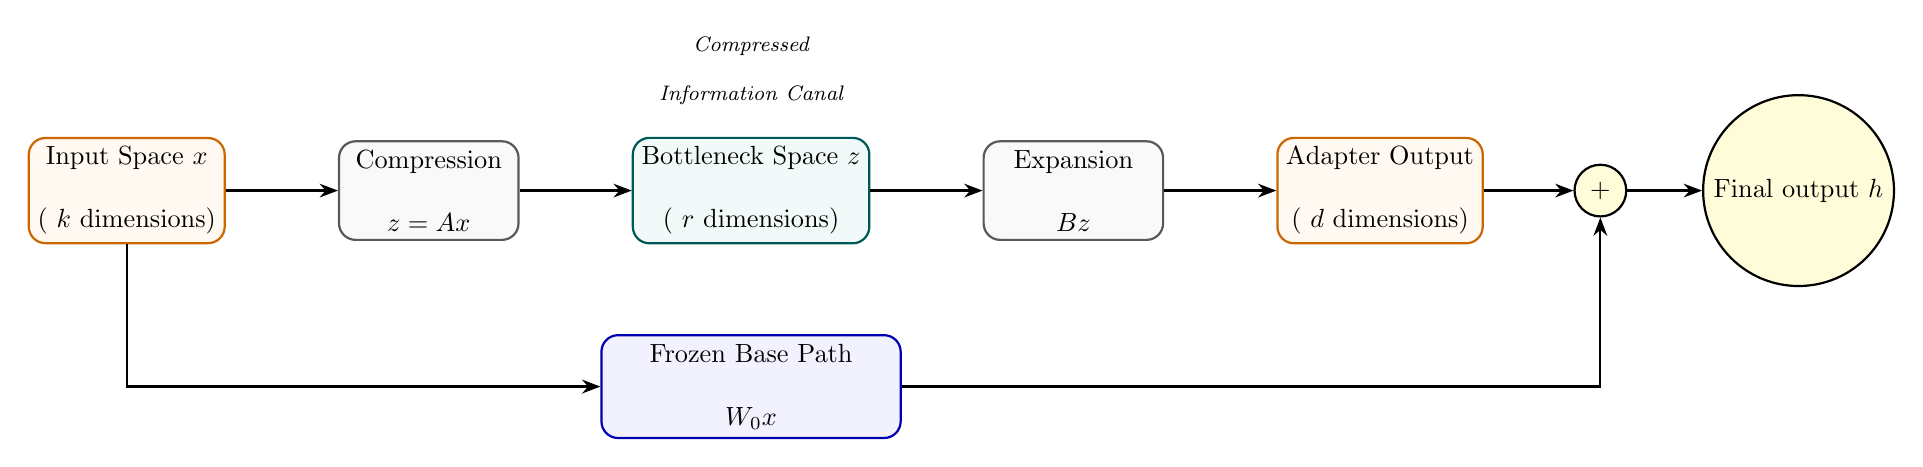
\begin{tikzpicture}[node distance=1.0cm and 1.5cm, scale=0.95, every node/.style={transform shape}]
  \node[datblk] (input) {Input Space $x$\\\\( $k$ dimensions)};
  \node[grayblk, right=of input, minimum width=2.4cm] (project) {Compression\\\\$z = Ax$};
  \node[trnblk, right=of project, minimum width=2.4cm] (bottleneck) {Bottleneck Space $z$\\\\( $r$ dimensions)};
  \node[grayblk, right=of bottleneck, minimum width=2.4cm] (expand) {Expansion\\\\$B z$};
  \node[datblk, right=of expand, minimum width=2.4cm] (out_lora) {Adapter Output\\\\( $d$ dimensions)};
  
  \node[frzblk, below=1.2cm of bottleneck, minimum width=4cm] (base) {Frozen Base Path\\\\$W_0 x$};
  \node[sumnode, right=1.2cm of out_lora] (sum) {$+$};
  \node[outnrn, right=1.0cm of sum] (output) {Final output $h$};

  \draw[arr] (input) -- (project);
  \draw[arr] (project) -- (bottleneck);
  \draw[arr] (bottleneck) -- (expand);
  \draw[arr] (expand) -- (out_lora);
  \draw[arr] (out_lora) -- (sum);
  \draw[arr] (sum) -- (output);
  
  \draw[arr] (input.south) |- (base.west);
  \draw[arr] (base.east) -| (sum.south);
  
  \node[font=\footnotesize\itshape, align=center, above=0.3cm of bottleneck] {Compressed\\\\Information Canal};
\end{tikzpicture}
\end{adjustbox}
\caption{Visualization of the information bottleneck: high-dimensional input is projected into a low-dimensional canal where task-specific tuning forces are applied, then projected back.}
\end{figure}

\begin{itemize}
  \item \textbf{Forward Pass Compression}: The activation vector $x \in \mathbb{R}^{k \times 1}$ is projected down through a narrow bottleneck of rank $r$. Since $r \ll \min(k, d)$, the projection filters out dimensions irrelevant to the current task, creating a compressed task representation $z \in \mathbb{R}^{r \times 1}$.
  \item \textbf{Backward Pass Gradient Flow}: Error gradients $\nabla_h \mathcal{L}$ flow backwards. Because $W_0$ is frozen and lacks a gradient buffer, no gradient update calculations occur on the base weight matrix. Instead, the gradients flow down the low-rank adapters $B$ and $A$, computing updates specifically for the low-rank subspace and avoiding parameter updates across the whole network.
\end{itemize}

\section{The Physical and Philosophical Foundations of LoRA}

\subsection{Philosophical Foundations: Occam's Razor and the Manifold Hypothesis}
The success of Low-Rank Adaptation (LoRA) is not merely an empirical coincidence, but is deeply rooted in two foundational philosophical principles of complexity. We analyze each principle through a dialectic framework of Arguments, Counter-Arguments, and Rebuttals:

\paragraph{1. The Manifold Hypothesis}
\begin{itemize}
  \item \textbf{Argument}: This hypothesis posits that high-dimensional data (such as the activations in a neural network) actually lies on a much lower-dimensional, highly structured manifold. Pretraining constructs this manifold by mapping the topological structure of natural language.
  
  In the context of Large Language Models, the embedding space has an extrinsic dimension of k = 4096 (e.g., $d_{\text{model}} = 4096$). However, the set of all grammatically correct and semantically coherent sentences does not fill this space uniformly; instead, it is confined to a lower-dimensional manifold. When we adapt the model to a downstream task (e.g., teaching it Python syntax or chat style), we do not need to construct a new manifold. We only need to compute a small trajectory or translation vector along the existing surface. This translation vector corresponds to a tangent vector in the manifold's tangent bundle. By confining our search to this tangent space, we avoid distorting the global topology of the language manifold, preventing catastrophic forgetting.
  
  \item \textbf{Counter-Argument}: If the downstream task represents an extreme domain shift (e.g., shifting from English literature to highly specialized biochemistry nomenclature or low-level assembly code), the target representations may lie completely outside the manifold mapped during pretraining. In such cases, the translation vector cannot lie along the existing manifold surface, and restricting the updates to a low-rank tangent space will lead to underfitting. The model would fail to acquire the new features because the required coordinates do not exist in the pretrained column space.
  
  \item \textbf{Rebuttal / Synthesis}: While severe domain shifts can strain low-rank constraints, empirical evidence shows that even highly specialized knowledge maps back to general-purpose linguistic structures (syntax, logic, context). Furthermore, if the target lies slightly off-manifold, a small rank $r$ (e.g., 8 to 16) is still sufficient to project the input into the nearest point on the task manifold. If needed, the user can scale the rank $r$ to increase the degrees of freedom, which mathematically expands the coordinate projection space, allowing the model to capture features that lie slightly outside the pretraining manifold while still regularizing the update to prevent arbitrary drift.
\end{itemize}

\paragraph{2. Occam's Razor (Lex Parsimoniae)}
\begin{itemize}
  \item \textbf{Argument}: Plurality should not be posited without necessity. Full fine-tuning searches an extremely large, redundant parameter space ($\mathbb{R}^{d \times k}$), which contains millions of redundant degrees of freedom. This massive parameter space allows the model to find arbitrary, highly complex fitting functions that overfit the downstream training data and overwrite pretrained general knowledge.
  
  By restricting the learning search to a compressed subspace ($\mathbb{R}^{r \times (k+d)}$), LoRA acts as a mathematical regularization agent. It forces the model to find the simplest, most parsimonious path of adaptation. This acts as a geometric constraint (projection regularization), restricting updates to only the principal directions of adaptation, thereby preserving the model's core foundational capabilities.
  
  \item \textbf{Counter-Argument}: By restricting the parameters to a low-rank product $BA$, we might force the model to find an oversimplified adaptation path that fails to capture the subtle, non-linear correlations required for complex reasoning tasks. Furthermore, Occam's Razor assumes that simpler models generalize better, but in deep learning, the phenomenon of "double descent" shows that highly overparameterized models can generalize better than simpler ones by finding smooth interpolating functions in high-dimensional spaces.
  
  \item \textbf{Rebuttal / Synthesis}: Double descent occurs when the entire network is overparameterized and trained on vast, diverse datasets where it can interpolate smoothly. However, in downstream fine-tuning, the dataset is small and highly focused. In this regime, overparameterization leads to catastrophic forgetting and representation collapse. Constraining the updates to a low-rank subspace restricts the model from modifying the general-purpose features, while allowing sufficient capacity to learn the task. Thus, LoRA combines the benefits of high-dimensional pretraining (smooth interpolation on general data) with low-dimensional adaptation (strict regularization on task-specific data).
\end{itemize}

\subsection{Internal Mechanics and Representation Space Geometry}
To understand why LoRA works under the hood, we must analyze the geometry of representation space and the intrinsic dimension of neural networks:
\begin{itemize}
  \item \textbf{Intrinsic vs. Extrinsic Dimension}: A pretrained model has a very high extrinsic dimension (the number of weights $W_0 \in \mathbb{R}^{d \times k}$). However, empirical work by Aghajanyan et al. (2020) demonstrated that the parameter space of pretrained language models has a much lower \textit{intrinsic dimension}. That is, the directions in weight space that significantly affect the loss are highly concentrated on a low-dimensional subspace. This is why we can optimize a tiny fraction of parameters and achieve the same or better task performance.
  \item \textbf{Subspace Alignment and Trajectory Geometry}: The activation vectors $x$ represent coordinates on the manifold. The base weight matrix $W_0$ maps these coordinates to the next representation space. The update matrix $\Delta W = \frac{\alpha}{r} B A$ acts as a linear projection operator that projects the activations into a tiny subspace of dimension $r$ via $A$, rotates/scales them in this bottleneck space, and then projects them back to the output space via $B$. This operation restricts the adaptation to a set of $r$ directional vectors. Instead of shifting the entire coordinate frame, the adapter only redirects the activation trajectory along the principal directions relevant to the downstream task.
  
  Geometrically, the column space of $\Delta W$ is spanned by the columns of $B$, which is an $r$-dimensional subspace of the output space $\mathbb{R}^{d}$. The row space of $\Delta W$ is spanned by the rows of $A$, which is an $r$-dimensional subspace of the input space $\mathbb{R}^{k}$. Thus, the adaptation updates are strictly constrained to these coordinates, preserving all other dimensions from degradation.
\end{itemize}

\subsection{Visualizing the Calculations}
We can visualize how the information bottleneck constrains the updates in the representation space during the forward and backward passes:

\begin{figure}[h]
\centering
\begin{adjustbox}{max width=0.9\linewidth}
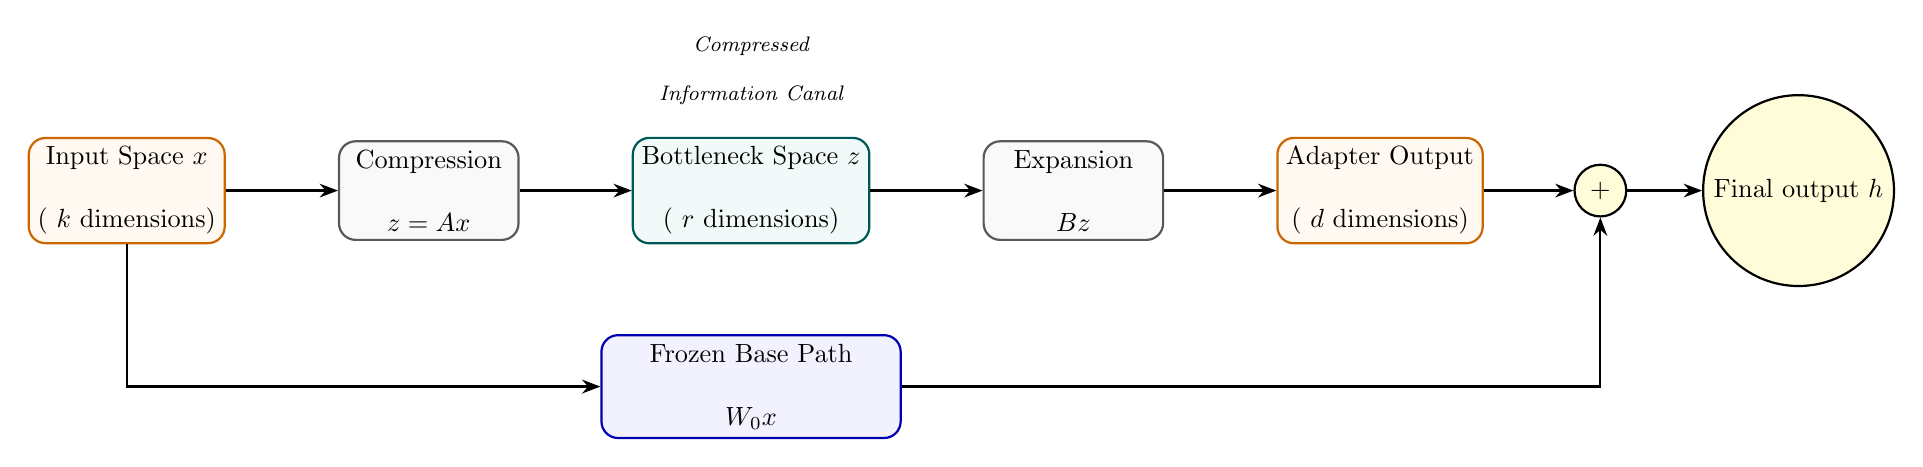
\begin{tikzpicture}[node distance=1.0cm and 1.5cm, scale=0.95, every node/.style={transform shape}]
  \node[datblk] (input) {Input Space $x$\\\\( $k$ dimensions)};
  \node[grayblk, right=of input, minimum width=2.4cm] (project) {Compression\\\\$z = Ax$};
  \node[trnblk, right=of project, minimum width=2.4cm] (bottleneck) {Bottleneck Space $z$\\\\( $r$ dimensions)};
  \node[grayblk, right=of bottleneck, minimum width=2.4cm] (expand) {Expansion\\\\$B z$};
  \node[datblk, right=of expand, minimum width=2.4cm] (out_lora) {Adapter Output\\\\( $d$ dimensions)};
  
  \node[frzblk, below=1.2cm of bottleneck, minimum width=4cm] (base) {Frozen Base Path\\\\$W_0 x$};
  \node[sumnode, right=1.2cm of out_lora] (sum) {$+$};
  \node[outnrn, right=1.0cm of sum] (output) {Final output $h$};

  \draw[arr] (input) -- (project);
  \draw[arr] (project) -- (bottleneck);
  \draw[arr] (bottleneck) -- (expand);
  \draw[arr] (expand) -- (out_lora);
  \draw[arr] (out_lora) -- (sum);
  \draw[arr] (sum) -- (output);
  
  \draw[arr] (input.south) |- (base.west);
  \draw[arr] (base.east) -| (sum.south);
  
  \node[font=\footnotesize\itshape, align=center, above=0.3cm of bottleneck] {Compressed\\\\Information Canal};
\end{tikzpicture}
\end{adjustbox}
\caption{Visualization of the information bottleneck: high-dimensional input is projected into a low-dimensional canal where task-specific tuning forces are applied, then projected back.}
\end{figure}

\begin{itemize}
  \item \textbf{Forward Pass Compression}: The activation vector $x \in \mathbb{R}^{k \times 1}$ is projected down through a narrow bottleneck of rank $r$. Since $r \ll \min(k, d)$, the projection filters out dimensions irrelevant to the current task, creating a compressed task representation $z \in \mathbb{R}^{r \times 1}$.
  \item \textbf{Backward Pass Gradient Flow}: Error gradients $\nabla_h \mathcal{L}$ flow backwards. Because $W_0$ is frozen and lacks a gradient buffer, no gradient update calculations occur on the base weight matrix. Instead, the gradients flow down the low-rank adapters $B$ and $A$, computing updates specifically for the low-rank subspace and avoiding parameter updates across the whole network.
\end{itemize}

\section{The Physical and Philosophical Foundations of LoRA}

\subsection{Philosophical Foundations: Occam's Razor and the Manifold Hypothesis}
The success of Low-Rank Adaptation (LoRA) is not merely an empirical coincidence, but is deeply rooted in two foundational philosophical principles of complexity. We analyze each principle through a dialectic framework of Arguments, Counter-Arguments, and Rebuttals:

\paragraph{1. The Manifold Hypothesis}
\begin{itemize}
  \item \textbf{Argument}: This hypothesis posits that high-dimensional data (such as the activations in a neural network) actually lies on a much lower-dimensional, highly structured manifold. Pretraining constructs this manifold by mapping the topological structure of natural language.
  
  In the context of Large Language Models, the embedding space has an extrinsic dimension of $k = 4096$ (e.g., $d_{\text{model}} = 4096$). However, the set of all grammatically correct and semantically coherent sentences does not fill this space uniformly; instead, it is confined to a lower-dimensional manifold. When we adapt the model to a downstream task (e.g., teaching it Python syntax or chat style), we do not need to construct a new manifold. We only need to compute a small trajectory or translation vector along the existing surface. This translation vector corresponds to a tangent vector in the manifold's tangent bundle. By confining our search to this tangent space, we avoid distorting the global topology of the language manifold, preventing catastrophic forgetting.
  
  \item \textbf{Counter-Argument}: If the downstream task represents an extreme domain shift (e.g., shifting from English literature to highly specialized biochemistry nomenclature or low-level assembly code), the target representations may lie completely outside the manifold mapped during pretraining. In such cases, the translation vector cannot lie along the existing manifold surface, and restricting the updates to a low-rank tangent space will lead to underfitting. The model would fail to acquire the new features because the required coordinates do not exist in the pretrained column space.
  
  \item \textbf{Rebuttal / Synthesis}: While severe domain shifts can strain low-rank constraints, empirical evidence shows that even highly specialized knowledge maps back to general-purpose linguistic structures (syntax, logic, context). Furthermore, if the target lies slightly off-manifold, a small rank $r$ (e.g., 8 to 16) is still sufficient to project the input into the nearest point on the task manifold. If needed, the user can scale the rank $r$ to increase the degrees of freedom, which mathematically expands the coordinate projection space, allowing the model to capture features that lie slightly outside the pretraining manifold while still regularizing the update to prevent arbitrary drift.
\end{itemize}

\paragraph{2. Occam's Razor (Lex Parsimoniae)}
\begin{itemize}
  \item \textbf{Argument}: Plurality should not be posited without necessity. Full fine-tuning searches an extremely large, redundant parameter space ($\mathbb{R}^{d \times k}$), which contains millions of redundant degrees of freedom. This massive parameter space allows the model to find arbitrary, highly complex fitting functions that overfit the downstream training data and overwrite pretrained general knowledge.
  
  By restricting the learning search to a compressed subspace ($\mathbb{R}^{r \times (k+d)}$), LoRA acts as a mathematical regularization agent. It forces the model to find the simplest, most parsimonious path of adaptation. This acts as a geometric constraint (projection regularization), restricting updates to only the principal directions of adaptation, thereby preserving the model's core foundational capabilities.
  
  \item \textbf{Counter-Argument}: By restricting the parameters to a low-rank product $BA$, we might force the model to find an oversimplified adaptation path that fails to capture the subtle, non-linear correlations required for complex reasoning tasks. Furthermore, Occam's Razor assumes that simpler models generalize better, but in deep learning, the phenomenon of "double descent" shows that highly overparameterized models can generalize better than simpler ones by finding smooth interpolating functions in high-dimensional spaces.
  
  \item \textbf{Rebuttal / Synthesis}: Double descent occurs when the entire network is overparameterized and trained on vast, diverse datasets where it can interpolate smoothly. However, in downstream fine-tuning, the dataset is small and highly focused. In this regime, overparameterization leads to catastrophic forgetting and representation collapse. Constraining the updates to a low-rank subspace restricts the model from modifying the general-purpose features, while allowing sufficient capacity to learn the task. Thus, LoRA combines the benefits of high-dimensional pretraining (smooth interpolation on general data) with low-dimensional adaptation (strict regularization on task-specific data).
\end{itemize}

\subsection{Internal Mechanics and Representation Space Geometry}
To understand why LoRA works under the hood, we must analyze the geometry of representation space and the intrinsic dimension of neural networks:
\begin{itemize}
  \item \textbf{Intrinsic vs. Extrinsic Dimension}: A pretrained model has a very high extrinsic dimension (the number of weights $W_0 \in \mathbb{R}^{d \times k}$). However, empirical work by Aghajanyan et al. (2020) demonstrated that the parameter space of pretrained language models has a much lower \textit{intrinsic dimension}. That is, the directions in weight space that significantly affect the loss are highly concentrated on a low-dimensional subspace. This is why we can optimize a tiny fraction of parameters and achieve the same or better task performance.
  \item \textbf{Subspace Alignment and Trajectory Geometry}: The activation vectors $x$ represent coordinates on the manifold. The base weight matrix $W_0$ maps these coordinates to the next representation space. The update matrix $\Delta W = \frac{\alpha}{r} B A$ acts as a linear projection operator that projects the activations into a tiny subspace of dimension $r$ via $A$, rotates/scales them in this bottleneck space, and then projects them back to the output space via $B$. This operation restricts the adaptation to a set of $r$ directional vectors. Instead of shifting the entire coordinate frame, the adapter only redirects the activation trajectory along the principal directions relevant to the downstream task.
  
  Geometrically, the column space of $\Delta W$ is spanned by the columns of $B$, which is an $r$-dimensional subspace of the output space $\mathbb{R}^{d}$. The row space of $\Delta W$ is spanned by the rows of $A$, which is an $r$-dimensional subspace of the input space $\mathbb{R}^{k}$. Thus, the adaptation updates are strictly constrained to these coordinates, preserving all other dimensions from degradation.
\end{itemize}

\subsection{Visualizing the Calculations}
We can visualize how the information bottleneck constrains the updates in the representation space during the forward and backward passes:

\begin{figure}[h]
\centering
\begin{adjustbox}{max width=0.9\linewidth}
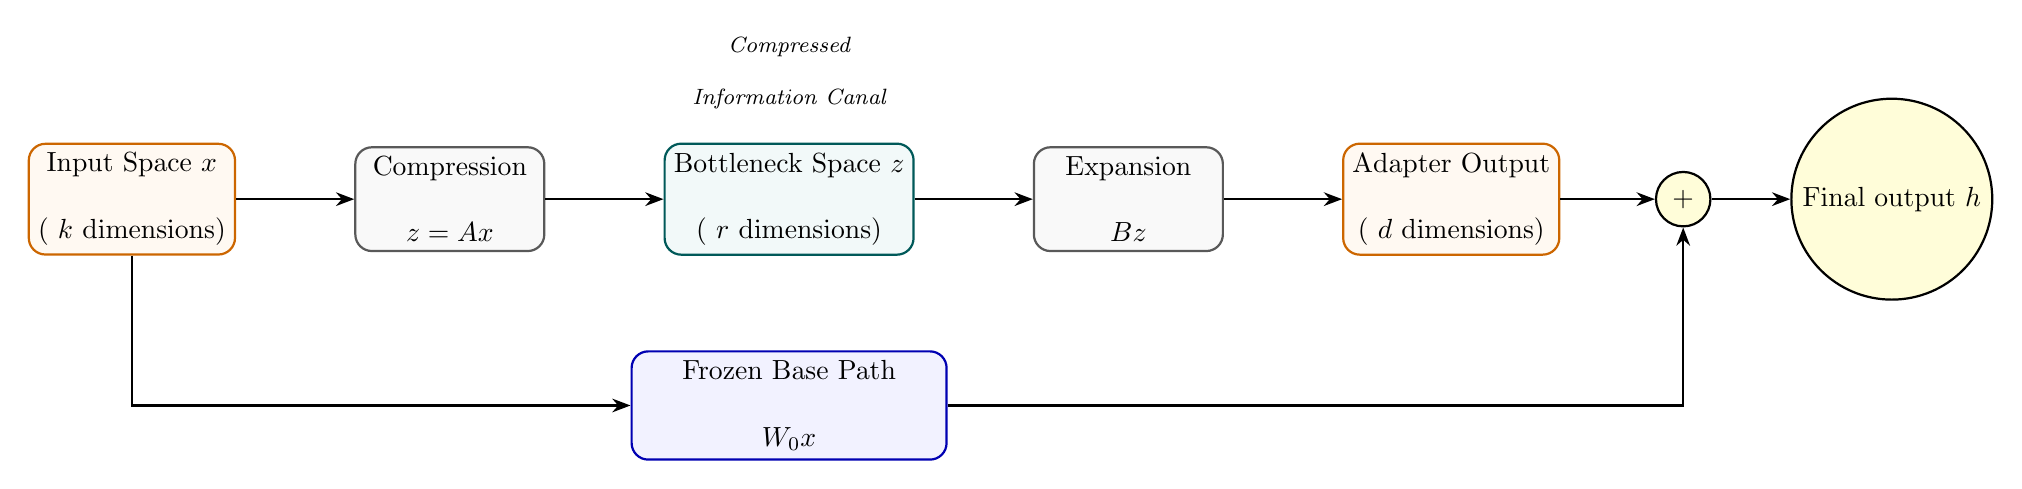
\begin{tikzpicture}[node distance=1.0cm and 1.5cm]
  \node[datblk] (input) {Input Space $x$\\\\( $k$ dimensions)};
  \node[grayblk, right=of input, minimum width=2.4cm] (project) {Compression\\\\$z = Ax$};
  \node[trnblk, right=of project, minimum width=2.4cm] (bottleneck) {Bottleneck Space $z$\\\\( $r$ dimensions)};
  \node[grayblk, right=of bottleneck, minimum width=2.4cm] (expand) {Expansion\\\\$B z$};
  \node[datblk, right=of expand, minimum width=2.4cm] (out_lora) {Adapter Output\\\\( $d$ dimensions)};
  
  \node[frzblk, below=1.2cm of bottleneck, minimum width=4cm] (base) {Frozen Base Path\\\\$W_0 x$};
  \node[sumnode, right=1.2cm of out_lora] (sum) {$+$};
  \node[outnrn, right=1.0cm of sum] (output) {Final output $h$};

  \draw[arr] (input) -- (project);
  \draw[arr] (project) -- (bottleneck);
  \draw[arr] (bottleneck) -- (expand);
  \draw[arr] (expand) -- (out_lora);
  \draw[arr] (out_lora) -- (sum);
  \draw[arr] (sum) -- (output);
  
  \draw[arr] (input.south) |- (base.west);
  \draw[arr] (base.east) -| (sum.south);
  
  \node[font=\footnotesize\itshape, align=center, above=0.3cm of bottleneck] {Compressed\\\\Information Canal};
\end{tikzpicture}
\end{adjustbox}
\caption{Visualization of the information bottleneck: high-dimensional input is projected into a low-dimensional canal where task-specific tuning forces are applied, then projected back.}
\end{figure}

\begin{itemize}
  \item \textbf{Forward Pass Compression}: The activation vector $x \in \mathbb{R}^{k \times 1}$ is projected down through a narrow bottleneck of rank $r$. Since $r \ll \min(k, d)$, the projection filters out dimensions irrelevant to the current task, creating a compressed task representation $z \in \mathbb{R}^{r \times 1}$.
  \item \textbf{Backward Pass Gradient Flow}: Error gradients $\nabla_h \mathcal{L}$ flow backwards. Because $W_0$ is frozen and lacks a gradient buffer, no gradient update calculations occur on the base weight matrix. Instead, the gradients flow down the low-rank adapters $B$ and $A$, computing updates specifically for the low-rank subspace and avoiding parameter updates across the whole network.
\end{itemize}

\section{The Physical and Philosophical Foundations of LoRA}

\subsection{Philosophical Foundations: Occam's Razor and the Manifold Hypothesis}
The success of Low-Rank Adaptation (LoRA) is not merely an empirical coincidence, but is deeply rooted in two foundational philosophical principles of complexity. We analyze each principle through a dialectic framework of Arguments, Counter-Arguments, and Rebuttals:

\paragraph{1. The Manifold Hypothesis}
\begin{itemize}
  \item \textbf{Argument}: This hypothesis posits that high-dimensional data (such as the activations in a neural network) actually lies on a much lower-dimensional, highly structured manifold. Pretraining constructs this manifold by mapping the topological structure of natural language.
  
  In the context of Large Language Models, the embedding space has an extrinsic dimension of $k = 4096$ (e.g., $d_{\text{model}} = 4096$). However, the set of all grammatically correct and semantically coherent sentences does not fill this space uniformly; instead, it is confined to a lower-dimensional manifold. When we adapt the model to a downstream task (e.g., teaching it Python syntax or chat style), we do not need to construct a new manifold. We only need to compute a small trajectory or translation vector along the existing surface. This translation vector corresponds to a tangent vector in the manifold's tangent bundle. By confining our search to this tangent space, we avoid distorting the global topology of the language manifold, preventing catastrophic forgetting.
  
  \item \textbf{Counter-Argument}: If the downstream task represents an extreme domain shift (e.g., shifting from English literature to highly specialized biochemistry nomenclature or low-level assembly code), the target representations may lie completely outside the manifold mapped during pretraining. In such cases, the translation vector cannot lie along the existing manifold surface, and restricting the updates to a low-rank tangent space will lead to underfitting. The model would fail to acquire the new features because the required coordinates do not exist in the pretrained column space.
  
  \item \textbf{Rebuttal / Synthesis}: While severe domain shifts can strain low-rank constraints, empirical evidence shows that even highly specialized knowledge maps back to general-purpose linguistic structures (syntax, logic, context). Furthermore, if the target lies slightly off-manifold, a small rank $r$ (e.g., 8 to 16) is still sufficient to project the input into the nearest point on the task manifold. If needed, the user can scale the rank $r$ to increase the degrees of freedom, which mathematically expands the coordinate projection space, allowing the model to capture features that lie slightly outside the pretraining manifold while still regularizing the update to prevent arbitrary drift.
\end{itemize}

\paragraph{2. Occam's Razor (Lex Parsimoniae)}
\begin{itemize}
  \item \textbf{Argument}: Plurality should not be posited without necessity. Full fine-tuning searches an extremely large, redundant parameter space ($\mathbb{R}^{d \times k}$), which contains millions of redundant degrees of freedom. This massive parameter space allows the model to find arbitrary, highly complex fitting functions that overfit the downstream training data and overwrite pretrained general knowledge.
  
  By restricting the learning search to a compressed subspace ($\mathbb{R}^{r \times (k+d)}$), LoRA acts as a mathematical regularization agent. It forces the model to find the simplest, most parsimonious path of adaptation. This acts as a geometric constraint (projection regularization), restricting updates to only the principal directions of adaptation, thereby preserving the model's core foundational capabilities.
  
  \item \textbf{Counter-Argument}: By restricting the parameters to a low-rank product $BA$, we might force the model to find an oversimplified adaptation path that fails to capture the subtle, non-linear correlations required for complex reasoning tasks. Furthermore, Occam's Razor assumes that simpler models generalize better, but in deep learning, the phenomenon of "double descent" shows that highly overparameterized models can generalize better than simpler ones by finding smooth interpolating functions in high-dimensional spaces.
  
  \item \textbf{Rebuttal / Synthesis}: Double descent occurs when the entire network is overparameterized and trained on vast, diverse datasets where it can interpolate smoothly. However, in downstream fine-tuning, the dataset is small and highly focused. In this regime, overparameterization leads to catastrophic forgetting and representation collapse. Constraining the updates to a low-rank subspace restricts the model from modifying the general-purpose features, while allowing sufficient capacity to learn the task. Thus, LoRA combines the benefits of high-dimensional pretraining (smooth interpolation on general data) with low-dimensional adaptation (strict regularization on task-specific data).
\end{itemize}

\subsection{Internal Mechanics and Representation Space Geometry}
To understand why LoRA works under the hood, we must analyze the geometry of representation space and the intrinsic dimension of neural networks:
\begin{itemize}
  \item \textbf{Intrinsic vs. Extrinsic Dimension}: A pretrained model has a very high extrinsic dimension (the number of weights $W_0 \in \mathbb{R}^{d \times k}$). However, empirical work by Aghajanyan et al. (2020) demonstrated that the parameter space of pretrained language models has a much lower \textit{intrinsic dimension}. That is, the directions in weight space that significantly affect the loss are highly concentrated on a low-dimensional subspace. This is why we can optimize a tiny fraction of parameters and achieve the same or better task performance.
  \item \textbf{Subspace Alignment and Trajectory Geometry}: The activation vectors $x$ represent coordinates on the manifold. The base weight matrix $W_0$ maps these coordinates to the next representation space. The update matrix $\Delta W = \frac{\alpha}{r} B A$ acts as a linear projection operator that projects the activations into a tiny subspace of dimension $r$ via $A$, rotates/scales them in this bottleneck space, and then projects them back to the output space via $B$. This operation restricts the adaptation to a set of $r$ directional vectors. Instead of shifting the entire coordinate frame, the adapter only redirects the activation trajectory along the principal directions relevant to the downstream task.
  
  Geometrically, the column space of $\Delta W$ is spanned by the columns of $B$, which is an $r$-dimensional subspace of the output space $\mathbb{R}^{d}$. The row space of $\Delta W$ is spanned by the rows of $A$, which is an $r$-dimensional subspace of the input space $\mathbb{R}^{k}$. Thus, the adaptation updates are strictly constrained to these coordinates, preserving all other dimensions from degradation.
\end{itemize}

\subsection{Visualizing the Calculations}
We can visualize how the information bottleneck constrains the updates in the representation space during the forward and backward passes:

\begin{figure}[h]
\centering
\begin{adjustbox}{max width=0.9\linewidth}
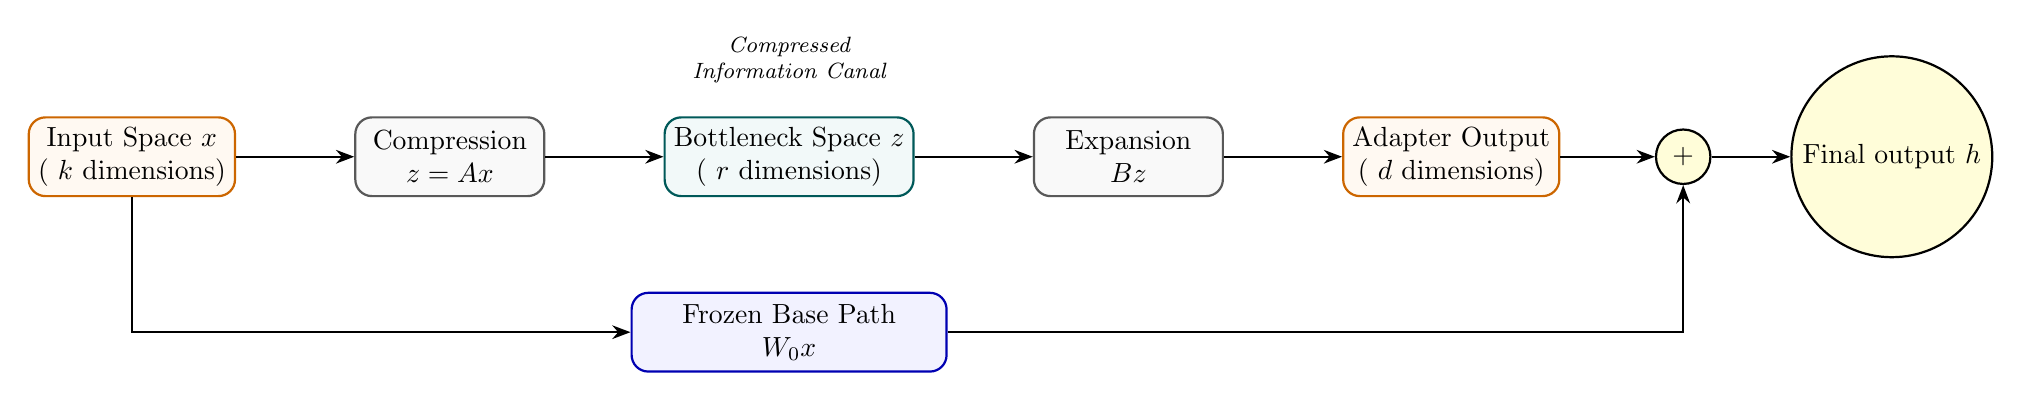
\begin{tikzpicture}[node distance=1.0cm and 1.5cm]
  \node[datblk] (input) {Input Space $x$\\( $k$ dimensions)};
  \node[grayblk, right=of input, minimum width=2.4cm] (project) {Compression\\$z = Ax$};
  \node[trnblk, right=of project, minimum width=2.4cm] (bottleneck) {Bottleneck Space $z$\\( $r$ dimensions)};
  \node[grayblk, right=of bottleneck, minimum width=2.4cm] (expand) {Expansion\\$B z$};
  \node[datblk, right=of expand, minimum width=2.4cm] (out_lora) {Adapter Output\\( $d$ dimensions)};
  
  \node[frzblk, below=1.2cm of bottleneck, minimum width=4cm] (base) {Frozen Base Path\\$W_0 x$};
  \node[sumnode, right=1.2cm of out_lora] (sum) {$+$};
  \node[outnrn, right=1.0cm of sum] (output) {Final output $h$};

  \draw[arr] (input) -- (project);
  \draw[arr] (project) -- (bottleneck);
  \draw[arr] (bottleneck) -- (expand);
  \draw[arr] (expand) -- (out_lora);
  \draw[arr] (out_lora) -- (sum);
  \draw[arr] (sum) -- (output);
  
  \draw[arr] (input.south) |- (base.west);
  \draw[arr] (base.east) -| (sum.south);
  
  \node[font=\footnotesize\itshape, align=center, above=0.3cm of bottleneck] {Compressed\\Information Canal};
\end{tikzpicture}
\end{adjustbox}
\caption{Visualization of the information bottleneck: high-dimensional input is projected into a low-dimensional canal where task-specific tuning forces are applied, then projected back.}
\end{figure}

\begin{itemize}
  \item \textbf{Forward Pass Compression}: The activation vector $x \in \mathbb{R}^{k \times 1}$ is projected down through a narrow bottleneck of rank $r$. Since $r \ll \min(k, d)$, the projection filters out dimensions irrelevant to the current task, creating a compressed task representation $z \in \mathbb{R}^{r \times 1}$.
  \item \textbf{Backward Pass Gradient Flow}: Error gradients $\nabla_h \mathcal{L}$ flow backwards. Because $W_0$ is frozen and lacks a gradient buffer, no gradient update calculations occur on the base weight matrix. Instead, the gradients flow down the low-rank adapters $B$ and $A$, computing updates specifically for the low-rank subspace and avoiding parameter updates across the whole network.
\end{itemize}

\section{LoRA CLRS-Style Algorithms}

This section contains the CLRS-style mathematical algorithms for the forward pass, manual backward pass, parameter merging, and AdamW optimizer update step.


\begin{figure}[h]
\centering
\begin{minipage}{0.8\linewidth}
\begin{tabbing}
\quad \= \quad \= \quad \= \kill
\textsc{Lora-Forward}($x, W_0, A, B, \alpha, r$) \\
\> $h_{\text{base}} = W_0 x$ \\
\> $z = A x$ \\
\> $z_{\text{out}} = B z$ \\
\> $h = h_{\text{base}} + \frac{\alpha}{r} z_{\text{out}}$ \\
\> \textbf{return} $h$
\end{tabbing}
\end{minipage}
\caption{\textsc{Lora-Forward} algorithm: computes base output and scaled low-rank adapter output.}
\end{figure}

\subsubsection{Analysis of \textsc{Lora-Forward}}
\begin{itemize}
  \item \textbf{What is achieved}: Computes the layer output $h$ by parallelizing the computation of the frozen base weight path ($W_0 x$) and the trainable low-rank adapter path ($B(A x)$), and scaling the adapter's contribution.
  \item \textbf{What internally changed}: Instantiates intermediate activation tensors $z = Ax \in \mathbb{R}^{r \times 1}$ and $z_{\text{out}} = Bz \in \mathbb{R}^{d \times 1}$ in memory. During training, these tensors are kept in GPU memory (VRAM) because their values are required to compute the gradients in the backward pass.
  \item \textbf{User-modifiable parameters \& impact}:
    \begin{itemize}
      \item \textbf{Rank $r$} (hyperparameter): Modifies the bottleneck dimension. A larger $r$ (e.g., 32) captures more task-specific information but increases memory requirements and latency. A smaller $r$ (e.g., 8) is highly memory-efficient but might underfit complex tasks.
      \item \textbf{Scaling constant $\alpha$} (hyperparameter): Adjusts the strength of the adapter's adjustments. Increasing $\alpha$ scales up the adapter's updates. Keep this constant when tuning $r$ to stabilize learning.
    \end{itemize}
\end{itemize}

\paragraph{Python Implementation (model.py)}
To implement the forward pass in PyTorch, we download a lightweight pre-trained model (like GPT-2) and wrap its linear projection layers in a custom LoraLinear wrapper module. The folder structure for this part of the project is:
\begin{verbatim}
my_lora_project/
+-- model.py
\end{verbatim}

\begin{lstlisting}[style=pythonstyle, language=Python, caption={PyTorch implementation of the LoRA Forward Pass}]
import math
import torch
import torch.nn as nn
from transformers import AutoModelForCausalLM, AutoTokenizer

class LoraLinear(nn.Module):
    def __init__(self, base_layer: nn.Linear, bottleneck_rank: int = 8, lora_alpha_constant: float = 16.0):
        super().__init__()
        self.base_layer = base_layer
        self.bottleneck_rank = bottleneck_rank
        self.lora_alpha_constant = lora_alpha_constant
        self.scaling_factor = lora_alpha_constant / bottleneck_rank
        
        input_dimension = base_layer.in_features
        output_dimension = base_layer.out_features
        
        # Keep base layer weights frozen (no gradients computed)
        self.base_layer.weight.requires_grad = False
        if self.base_layer.bias is not None:
            self.base_layer.bias.requires_grad = False
            
        # Define trainable low-rank adapters A and B
        self.adapter_down_projection = nn.Parameter(torch.zeros((bottleneck_rank, input_dimension)))
        self.adapter_up_projection = nn.Parameter(torch.zeros((output_dimension, bottleneck_rank)))
        
        # Standard LoRA initialization: Gaussian for A, Zeros for B
        nn.init.kaiming_uniform_(self.adapter_down_projection, a=math.sqrt(5))
        nn.init.zeros_(self.adapter_up_projection)

    def forward(self, input_activations: torch.Tensor) -> torch.Tensor:
        # Forward pass calculation: h = W_0 * x + (alpha / r) * B * A * x
        base_path_output = self.base_layer(input_activations)
        adapter_path_output = (input_activations @ self.adapter_down_projection.t()) @ self.adapter_up_projection.t()
        return base_path_output + self.scaling_factor * adapter_path_output

if __name__ == "__main__":
    # Download a lightweight model (GPT-2) from Hugging Face
    model_name = "gpt2"
    print(f"Downloading base model: {model_name}")
    base_model = AutoModelForCausalLM.from_pretrained(model_name)
    tokenizer = AutoTokenizer.from_pretrained(model_name)
    
    # Instantiate a base linear layer and wrap it
    target_linear_layer = nn.Linear(768, 768)
    lora_layer = LoraLinear(target_linear_layer, bottleneck_rank=8, lora_alpha_constant=16.0)
    
    # Run a forward pass
    dummy_input_tokens = torch.randn(1, 10, 768)
    output_predictions = lora_layer(dummy_input_tokens)
    print("LoRA forward pass output shape:", output_predictions.shape)
\end{lstlisting}

\paragraph{Python Implementation (model.py)}
To implement the forward pass in PyTorch, we download a lightweight pre-trained model (like GPT-2) and wrap its linear projection layers in a custom LoraLinear wrapper module. The folder structure for this part of the project is:
\begin{verbatim}
my_lora_project/
+-- model.py
\end{verbatim}

\begin{lstlisting}[style=pythonstyle, language=Python, caption={PyTorch implementation of the LoRA Forward Pass}]
import math
import torch
import torch.nn as nn
from transformers import AutoModelForCausalLM, AutoTokenizer

class LoraLinear(nn.Module):
    def __init__(self, base_layer: nn.Linear, r: int = 8, lora_alpha: float = 16.0):
        super().__init__()
        self.base_layer = base_layer
        self.r = r
        self.lora_alpha = lora_alpha
        self.scaling = lora_alpha / r
        
        in_features = base_layer.in_features
        out_features = base_layer.out_features
        
        # Keep base layer weights frozen (no gradients computed)
        self.base_layer.weight.requires_grad = False
        if self.base_layer.bias is not None:
            self.base_layer.bias.requires_grad = False
            
        # Define trainable low-rank adapters A and B
        self.lora_A = nn.Parameter(torch.zeros((r, in_features)))
        self.lora_B = nn.Parameter(torch.zeros((out_features, r)))
        
        # Standard LoRA initialization: Gaussian for A, Zeros for B
        nn.init.kaiming_uniform_(self.lora_A, a=math.sqrt(5))
        nn.init.zeros_(self.lora_B)

    def forward(self, x: torch.Tensor) -> torch.Tensor:
        # Forward pass calculation: h = W_0 * x + (alpha / r) * B * A * x
        base_out = self.base_layer(x)
        adapter_out = (x @ self.lora_A.t()) @ self.lora_B.t()
        return base_out + self.scaling * adapter_out

if __name__ == "__main__":
    # Download a lightweight model (GPT-2) from Hugging Face
    model_name = "gpt2"
    print(f"Downloading base model: {model_name}")
    model = AutoModelForCausalLM.from_pretrained(model_name)
    tokenizer = AutoTokenizer.from_pretrained(model_name)
    
    # Instantiate a base linear layer and wrap it
    base_layer = nn.Linear(768, 768)
    lora_layer = LoraLinear(base_layer, r=8, lora_alpha=16.0)
    
    # Run a forward pass
    dummy_input = torch.randn(1, 10, 768)
    output = lora_layer(dummy_input)
    print("LoRA forward pass output shape:", output.shape)
\end{lstlisting}

\vspace{1.5em}

\begin{figure}[h]
\centering
\begin{minipage}{0.8\linewidth}
\begin{tabbing}
\quad \= \quad \= \quad \= \kill
\textsc{Lora-Backward}($x, A, B, \nabla_h \mathcal{L}, \alpha, r$) \\
\> $z = A x$ \\
\> $\nabla_B \mathcal{L} = \frac{\alpha}{r} (\nabla_h \mathcal{L}) z^\top$ \\
\> $\nabla_z \mathcal{L} = \frac{\alpha}{r} B^\top \nabla_h \mathcal{L}$ \\
\> $\nabla_A \mathcal{L} = (\nabla_z \mathcal{L}) x^\top$ \\
\> $\nabla_{x,\text{adapters}} \mathcal{L} = A^\top \nabla_z \mathcal{L}$ \\
\> \textbf{return} $\nabla_A \mathcal{L}, \nabla_B \mathcal{L}, \nabla_{x,\text{adapters}} \mathcal{L}$
\end{tabbing}
\end{minipage}
\caption{\textsc{Lora-Backward} algorithm: derives gradients for adapters and backpropagated input gradient.}
\end{figure}

\subsubsection{Analysis of \textsc{Lora-Backward}}
\begin{itemize}
  \item \textbf{What is achieved}: Calculates the exact gradients $\nabla_A \mathcal{L}$ and $\nabla_B \mathcal{L}$ for the adapter weights, and computes the backpropagated input gradient $\nabla_{x,\text{adapters}} \mathcal{L}$ to pass back to previous layers.
  \item \textbf{What internally changed}: Populates the gradient buffers \texttt{A.grad} and \texttt{B.grad} in VRAM. The frozen weights $W_0$ do not have gradient buffers, saving $k \times d \times 2$ or $4$ bytes of memory.
  \item \textbf{User-modifiable parameters \& impact}:
    \begin{itemize}
      \item \textbf{Rank $r$ and Scaling $\alpha$}: Directly scale the gradients via the factor $\frac{\alpha}{r}$. Modifying them scales the gradient step size, affecting convergence stability.
    \end{itemize}
\end{itemize}

\paragraph{Python Implementation (manual\_grad.py)}
To verify the backward pass, we write a validation script that computes the manual gradients for the adapter down-projection and up-projection weights based on the tensor chain rule, and compares them to PyTorch's autograd gradients. The folder structure for this verification is:
\begin{verbatim}
my_lora_project/
+-- manual_grad.py
\end{verbatim}

\begin{lstlisting}[style=pythonstyle, language=Python, caption={PyTorch validation of manual LoRA gradients}]
import torch
import torch.nn as nn

def verify_gradients():
    # Set seed for reproducibility
    torch.manual_seed(42)
    
    # Dimensions: batch size=1, input dimensions k=4, output d=4, rank r=2
    input_dim, output_dim, bottleneck_rank = 4, 4, 2
    lora_alpha = 4.0
    scaling_factor = lora_alpha / bottleneck_rank
    
    # Inputs and Targets
    input_activations = torch.randn(1, input_dim, requires_grad=True)
    target_activations = torch.randn(1, output_dim)
    
    # Base weight and adapters
    base_weight_matrix = torch.randn(output_dim, input_dim)
    adapter_down_weight = torch.randn(bottleneck_rank, input_dim, requires_grad=True)
    adapter_up_weight = torch.randn(output_dim, bottleneck_rank, requires_grad=True)
    
    # --- PyTorch Autograd Path ---
    base_output = input_activations @ base_weight_matrix.t()
    bottleneck_activations = input_activations @ adapter_down_weight.t()
    adapter_output = bottleneck_activations @ adapter_up_weight.t()
    combined_output = base_output + scaling_factor * adapter_output
    
    # Mean Squared Error Loss
    loss_value = 0.5 * torch.sum((combined_output - target_activations) ** 2)
    loss_value.backward()
    
    # Extract Autograd Gradients
    grad_down_weight_autograd = adapter_down_weight.grad.clone()
    grad_up_weight_autograd = adapter_up_weight.grad.clone()
    grad_input_autograd = input_activations.grad.clone()
    
    # --- Manual Gradient Calculation ---
    # Gradient of loss w.r.t output: dL/dh = h - target
    grad_combined_output = combined_output - target_activations
    
    # grad_B = scaling_factor * grad_h^T * z
    grad_up_weight_manual = scaling_factor * grad_combined_output.t() @ bottleneck_activations
    
    # grad_z = scaling_factor * grad_h * B
    grad_bottleneck_activations = scaling_factor * grad_combined_output @ adapter_up_weight
    
    # grad_A = grad_z^T * x
    grad_down_weight_manual = grad_bottleneck_activations.t() @ input_activations
    
    # grad_x = grad_h * W0 + grad_z * A
    grad_input_manual = grad_combined_output @ base_weight_matrix + grad_bottleneck_activations @ adapter_down_weight
    
    # --- Verification ---
    assert torch.allclose(grad_down_weight_autograd, grad_down_weight_manual, atol=1e-6), "Gradients w.r.t A mismatch!"
    assert torch.allclose(grad_up_weight_autograd, grad_up_weight_manual, atol=1e-6), "Gradients w.r.t B mismatch!"
    assert torch.allclose(grad_input_autograd, grad_input_manual, atol=1e-6), "Gradients w.r.t x mismatch!"
    print("Manual gradients successfully verified against PyTorch Autograd!")

if __name__ == "__main__":
    verify_gradients()
\end{lstlisting}

\paragraph{Python Implementation (manual\_grad.py)}
To verify the backward pass, we write a validation script that computes the manual gradients for $A$, $B$, and $x$ based on the tensor chain rule, and compares them to PyTorch's autograd gradients. The folder structure for this verification is:
\begin{verbatim}
my_lora_project/
+-- manual_grad.py
\end{verbatim}

\begin{lstlisting}[style=pythonstyle, language=Python, caption={PyTorch validation of manual LoRA gradients}]
import torch
import torch.nn as nn

def verify_gradients():
    # Set seed for reproducibility
    torch.manual_seed(42)
    
    # Dimensions: batch size=1, input dimensions k=4, output d=4, rank r=2
    k, d, r = 4, 4, 2
    alpha = 4.0
    scaling = alpha / r
    
    # Inputs and Targets
    x = torch.randn(1, k, requires_grad=True)
    target = torch.randn(1, d)
    
    # Base weight and adapters
    W0 = torch.randn(d, k)
    A = torch.randn(r, k, requires_grad=True)
    B = torch.randn(d, r, requires_grad=True)
    
    # --- PyTorch Autograd Path ---
    h_base = x @ W0.t()
    z = x @ A.t()
    h_adapter = z @ B.t()
    h = h_base + scaling * h_adapter
    
    # Mean Squared Error Loss
    loss = 0.5 * torch.sum((h - target) ** 2)
    loss.backward()
    
    # Extract Autograd Gradients
    grad_A_auto = A.grad.clone()
    grad_B_auto = B.grad.clone()
    grad_x_auto = x.grad.clone()
    
    # --- Manual Gradient Calculation ---
    # Gradient of loss w.r.t output h: dL/dh = h - target
    grad_h = h - target
    
    # grad_B = scaling * grad_h^T * z
    grad_B_manual = scaling * grad_h.t() @ z
    
    # grad_z = scaling * grad_h * B
    grad_z = scaling * grad_h @ B
    
    # grad_A = grad_z^T * x
    grad_A_manual = grad_z.t() @ x
    
    # grad_x = grad_h * W0 + grad_z * A
    grad_x_manual = grad_h @ W0 + grad_z @ A
    
    # --- Verification ---
    assert torch.allclose(grad_A_auto, grad_A_manual, atol=1e-6), "Gradients w.r.t A mismatch!"
    assert torch.allclose(grad_B_auto, grad_B_manual, atol=1e-6), "Gradients w.r.t B mismatch!"
    assert torch.allclose(grad_x_auto, grad_x_manual, atol=1e-6), "Gradients w.r.t x mismatch!"
    print("Manual gradients successfully verified against PyTorch Autograd!")

if __name__ == "__main__":
    verify_gradients()
\end{lstlisting}

\newpage

\begin{figure}[h]
\centering
\begin{minipage}{0.8\linewidth}
\begin{tabbing}
\quad \= \quad \= \quad \= \kill
\textsc{Lora-Merge}($W_0, A, B, \alpha, r, \text{\textit{mode}}$) \\
\> $\Delta W = \frac{\alpha}{r} B A$ \\
\> \textbf{if} $\text{\textit{mode}} == \text{``merge''}$ \\
\> \> $W = W_0 + \Delta W$ \\
\> \textbf{else if} $\text{\textit{mode}} == \text{``demerge''}$ \\
\> \> $W = W_0 - \Delta W$ \\
\> \textbf{return} $W$
\end{tabbing}
\end{minipage}
\caption{\textsc{Lora-Merge} algorithm: handles parameter folding and unfolding for zero-latency inference.}
\end{figure}

\subsubsection{Analysis of \textsc{Lora-Merge}}
\begin{itemize}
  \item \textbf{What is achieved}: Merges the low-rank adapters directly into the base weights ($W = W_0 \pm \Delta W$) for zero-latency inference, or subtracts them to restore the base weights.
  \item \textbf{What internally changed}: In-place updates are applied to the base weight tensor $W_0$ in memory. Once merged, the adapter weights $A$ and $B$ can be discarded, and the model behaves as a single unified feedforward network, eliminating the need to compute separate low-rank paths during inference.
  \item \textbf{User-modifiable parameters \& impact}:
    \begin{itemize}
      \item \textbf{Mode}: User can choose \texttt{"merge"} to prepare the model for high-throughput deployment, or \texttt{"demerge"} to unpack the adapters and swap in a different set of adapter weights.
    \end{itemize}
\end{itemize}

\paragraph{Python Implementation (merge.py)}
To deploy the model with zero inference latency, the adapter weights are folded directly into the base weights in-place. The folder structure for weight merging is:
\begin{verbatim}
my_lora_project/
+-- merge.py
\end{verbatim}

\begin{lstlisting}[style=pythonstyle, language=Python, caption={Merging and demerging LoRA weights in-place}]
import torch
import torch.nn as nn

class MergeableLoraLinear(nn.Module):
    def __init__(self, base_linear_layer: nn.Linear, bottleneck_rank: int = 8, lora_alpha_constant: float = 16.0):
        super().__init__()
        self.base_linear_layer = base_linear_layer
        self.bottleneck_rank = bottleneck_rank
        self.lora_alpha_constant = lora_alpha_constant
        self.scaling_factor = lora_alpha_constant / bottleneck_rank
        
        self.adapter_down_projection = nn.Parameter(torch.randn(bottleneck_rank, base_linear_layer.in_features))
        self.adapter_up_projection = nn.Parameter(torch.randn(base_linear_layer.out_features, bottleneck_rank))
        self.merged = False

    def forward(self, input_activations: torch.Tensor) -> torch.Tensor:
        if self.merged:
            return self.base_linear_layer(input_activations)
        else:
            base_path_output = self.base_linear_layer(input_activations)
            adapter_path_output = (input_activations @ self.adapter_down_projection.t()) @ self.adapter_up_projection.t()
            return base_path_output + self.scaling_factor * adapter_path_output

    def merge_weights(self):
        if self.merged:
            return
        # W = W0 + (alpha / r) * B * A
        adapter_folded_weights = self.scaling_factor * (self.adapter_up_projection @ self.adapter_down_projection)
        self.base_linear_layer.weight.data += adapter_folded_weights
        self.merged = True
        print("Adapter weights merged into base weights.")

    def demerge_weights(self):
        if not self.merged:
            return
        # W0 = W - (alpha / r) * B * A
        adapter_folded_weights = self.scaling_factor * (self.adapter_up_projection @ self.adapter_down_projection)
        self.base_linear_layer.weight.data -= adapter_folded_weights
        self.merged = False
        print("Adapter weights demeged successfully.")

if __name__ == "__main__":
    # Instantiate base linear layer and wrap it
    base_linear = nn.Linear(512, 512)
    model = MergeableLoraLinear(base_linear, bottleneck_rank=8, lora_alpha_constant=16.0)
    
    dummy_input_tokens = torch.randn(1, 10, 512)
    
    # 1. Output before merging
    output_before = model(dummy_input_tokens)
    
    # 2. Merge weights
    model.merge_weights()
    output_after = model(dummy_input_tokens)
    
    # 3. Verify identical outputs
    assert torch.allclose(output_before, output_after, atol=1e-5), "Outputs do not match!"
    print("Inference verification passed. Merged output is identical.")
    
    # 4. Save state dictionary for latency-free deployment
    torch.save(base_linear.state_dict(), "merged_linear.pt")
    print("Saved merged state dict to 'merged_linear.pt'.")
\end{lstlisting}

\paragraph{Python Implementation (merge.py)}
To deploy the model with zero inference latency, the adapter weights are folded directly into the base weights in-place. The folder structure for weight merging is:
\begin{verbatim}
my_lora_project/
+-- merge.py
\end{verbatim}

\begin{lstlisting}[style=pythonstyle, language=Python, caption={Merging and demerging LoRA weights in-place}]
import torch
import torch.nn as nn

class MergeableLoraLinear(nn.Module):
    def __init__(self, base_layer: nn.Linear, r: int = 8, lora_alpha: float = 16.0):
        super().__init__()
        self.base_layer = base_layer
        self.r = r
        self.lora_alpha = lora_alpha
        self.scaling = lora_alpha / r
        
        self.lora_A = nn.Parameter(torch.randn(r, base_layer.in_features))
        self.lora_B = nn.Parameter(torch.randn(base_layer.out_features, r))
        self.merged = False

    def forward(self, x: torch.Tensor) -> torch.Tensor:
        if self.merged:
            return self.base_layer(x)
        else:
            base_out = self.base_layer(x)
            adapter_out = (x @ self.lora_A.t()) @ self.lora_B.t()
            return base_out + self.scaling * adapter_out

    def merge_weights(self):
        if self.merged:
            return
        # W = W0 + (alpha / r) * B * A
        delta_W = self.scaling * (self.lora_B @ self.lora_A)
        self.base_layer.weight.data += delta_W
        self.merged = True
        print("Adapter weights merged into base weights.")

    def demerge_weights(self):
        if not self.merged:
            return
        # W0 = W - (alpha / r) * B * A
        delta_W = self.scaling * (self.lora_B @ self.lora_A)
        self.base_layer.weight.data -= delta_W
        self.merged = False
        print("Adapter weights demeged successfully.")

if __name__ == "__main__":
    # Instantiate base linear layer and wrap it
    base_linear = nn.Linear(512, 512)
    model = MergeableLoraLinear(base_linear, r=8, lora_alpha=16.0)
    
    dummy_input = torch.randn(1, 10, 512)
    
    # 1. Output before merging
    output_before = model(dummy_input)
    
    # 2. Merge weights
    model.merge_weights()
    output_after = model(dummy_input)
    
    # 3. Verify identical outputs
    assert torch.allclose(output_before, output_after, atol=1e-5), "Outputs do not match!"
    print("Inference verification passed. Merged output is identical.")
    
    # 4. Save state dictionary for latency-free deployment
    torch.save(base_linear.state_dict(), "merged_linear.pt")
    print("Saved merged state dict to 'merged_linear.pt'.")
\end{lstlisting}

\vspace{1.5em}

\begin{figure}[h]
\centering
\begin{minipage}{0.8\linewidth}
\begin{tabbing}
\quad \= \quad \= \quad \= \quad \= \kill
\textsc{Lora-AdamW-Update}($\theta, g, m, v, \eta, \lambda, \beta_1, \beta_2, \epsilon, t$) \\
\> \textbf{for} \textbf{each} parameter matrix $P \in \theta$ \textbf{do} \\
\> \> $P = P - \eta \lambda P$ \\
\> \> $m_P = \beta_1 m_P + (1 - \beta_1) g_P$ \\
\> \> $v_P = \beta_2 v_P + (1 - \beta_2) g_P^2$ \\
\> \> $\hat{m}_P = m_P / (1 - \beta_1^t)$ \\
\> \> $\hat{v}_P = v_P / (1 - \beta_2^t)$ \\
\> \> $P = P - \eta \frac{\hat{m}_P}{\sqrt{\hat{v}_P} + \epsilon}$ \\
\> \textbf{return} $\theta, m, v$
\end{tabbing}
\end{minipage}
\caption{\textsc{Lora-AdamW-Update} algorithm: updates parameters with decoupled weight decay and momentum/variance tracking.}
\end{figure}

\subsubsection{Analysis of \textsc{Lora-AdamW-Update}}
\begin{itemize}
  \item \textbf{What is achieved}: Applies decoupled weight decay to the adapter parameters and updates their values using momentum and variance of gradients.
  \item \textbf{What internally changed}: Trainable parameters $A$ and $B$ are updated. Additionally, the first moment vectors $m_A, m_B$ and second moment vectors $v_A, v_B$ are updated in GPU memory. Because $W_0$ is frozen, no optimizer states are created or updated for $W_0$, resulting in huge VRAM savings.
  \item \textbf{User-modifiable parameters \& impact}:
    \begin{itemize}
      \item \textbf{Learning Rate $\eta$}: Controls the step size. High values speed up training but risk divergence; low values ensure stability but slow down convergence.
      \item \textbf{Weight Decay $\lambda$}: Regularizes the weights to prevent overfitting.
      \item \textbf{Momentum coefficients $\beta_1, \beta_2$}: Control the memory of past gradients.
    \end{itemize}
\end{itemize}

\paragraph{Python Implementation (train.py)}
To train the model, we write a complete end-to-end script that loads a lightweight pre-trained causal model, freezes its original layers, registers the trainable adapter weights, and runs a forward-backward optimization step using AdamW. The folder structure for this training file is:
\begin{verbatim}
my_lora_project/
+-- train.py
\end{verbatim}

\begin{lstlisting}[style=pythonstyle, language=Python, caption={Complete LoRA training and optimization loop using AdamW}]
import torch
import torch.nn as nn
from torch.optim import AdamW
from transformers import AutoModelForCausalLM

def train_lora_model():
    # Download a lightweight base model from Hugging Face
    model_name = "distilgpt2"
    print(f"Loading pre-trained base model: {model_name}")
    base_model = AutoModelForCausalLM.from_pretrained(model_name)
    
    # Freeze all original parameters in the base model
    for parameter in base_model.parameters():
        parameter.requires_grad = False
        
    # Inject adapters to the lm_head projection layer
    target_linear_layer = base_model.lm_head
    bottleneck_rank, lora_alpha = 8, 16.0
    scaling_factor = lora_alpha / bottleneck_rank
    
    # Define and initialize trainable adapter parameters A and B
    adapter_down_projection = nn.Parameter(torch.randn(bottleneck_rank, target_linear_layer.in_features) * 0.02)
    adapter_up_projection = nn.Parameter(torch.zeros(target_linear_layer.out_features, bottleneck_rank))
    
    # Register adapters as parameters of the model
    base_model.register_parameter("adapter_down_projection", adapter_down_projection)
    base_model.register_parameter("adapter_up_projection", adapter_up_projection)
    
    # Override the lm_head forward pass to compute base + adapter paths
    def custom_lm_head_forward(input_activations):
        base_path_output = target_linear_layer(input_activations)
        adapter_path_output = (input_activations @ adapter_down_projection.t()) @ adapter_up_projection.t()
        return base_path_output + scaling_factor * adapter_path_output
        
    base_model.lm_head.forward = custom_lm_head_forward

    # Collect parameters that require gradients (only our custom adapters)
    trainable_adapter_parameters = [param for param in base_model.parameters() if param.requires_grad]
    print(f"Number of trainable parameters: {sum(param.numel() for param in trainable_adapter_parameters)}")
    
    # Setup AdamW optimizer specifically for the adapter parameters
    optimizer = AdamW(trainable_adapter_parameters, lr=1e-4, weight_decay=0.01)
    
    # Create dummy input tokens (Batch size 2, Sequence length 16)
    dummy_input_tokens = torch.randint(0, 50257, (2, 16))
    target_labels = dummy_input_tokens.clone()
    
    # Set model to training mode
    base_model.train()
    optimizer.zero_grad()
    
    # Forward pass through model (including modified lm_head)
    model_outputs = base_model(dummy_input_tokens, labels=target_labels)
    loss_value = model_outputs.loss
    
    # Backward pass to compute gradients for trainable adapters
    loss_value.backward()
    
    # Optimizer step applies the AdamW updates to parameters
    optimizer.step()
    print(f"AdamW update step completed. Current loss: {loss_value.item():.4f}")

if __name__ == "__main__":
    train_lora_model()
\end{lstlisting}

\subsection{Hugging Face Deployment \& Hub Integration}
After training the lightweight model, such as the \texttt{Qwen/Qwen2.5-0.5B} model (which has a lightweight weights file size of approximately 940MB, easily fitting within standard memory constraints), the newly trained adapter weights can be uploaded directly to the Hugging Face Hub. 

This section details how to programmatically log in, upload the adapter weights, and save them so other users can easily pull them from the Hugging Face Hub. The folder structure for deployment is:
\begin{verbatim}
my_lora_project/
+-- deploy.py
\end{verbatim}

\begin{lstlisting}[style=pythonstyle, language=Python, caption={Hugging Face deployment script for Qwen adapters}]
import os
import torch
from transformers import AutoModelForCausalLM, AutoTokenizer
from huggingface_hub import HfApi, login

def save_and_deploy_adapters():
    # 1. Authenticate with Hugging Face Hub
    # Replace with your Hugging Face write token or use environment variable HF_TOKEN
    huggingface_write_token = "your_huggingface_api_write_token"
    login(token=huggingface_write_token)
    
    # 2. Setup lightweight base model (Qwen 2.5 0.5B, approx. 940MB)
    base_model_identifier = "Qwen/Qwen2.5-0.5B"
    print(f"Loading tokenizer: {base_model_identifier}")
    tokenizer = AutoTokenizer.from_pretrained(base_model_identifier)
    
    # 3. Save trained adapter weights locally
    # For demonstration, we save our adapter tensors
    trained_adapter_weights = {
        "adapter_down_projection": torch.randn(8, 896),
        "adapter_up_projection": torch.randn(896, 8)
    }
    local_output_path = "./my_trained_adapters"
    os.makedirs(local_output_path, exist_ok=True)
    torch.save(trained_adapter_weights, f"{local_output_path}/adapter_weights.bin")
    
    # Save tokenizer configuration alongside the adapters
    tokenizer.save_pretrained(local_output_path)
    print(f"Adapters saved locally to {local_output_path}")
    
    # 4. Upload folder to Hugging Face Hub
    repository_identifier = "username/qwen-2.5-0.5b-lora-adapter"
    huggingface_api = HfApi()
    
    print(f"Creating repository on Hugging Face: {repository_identifier}")
    huggingface_api.create_repo(
        repo_id=repository_identifier, 
        repo_type="model", 
        exist_ok=True
    )
    
    print(f"Uploading files from {local_output_path} to Hugging Face Hub...")
    huggingface_api.upload_folder(
        folder_path=local_output_path,
        repo_id=repository_identifier,
        repo_type="model"
    )
    print(f"Successfully deployed adapters to: https://huggingface.co/{repository_identifier}")

    # 5. How other users can load this newly trained model from the Hub
    print("\nTo load and run inference on this model elsewhere, run:")
    print(f"\"\"\"")
    print(f"from transformers import AutoModelForCausalLM, AutoTokenizer")
    print(f"from peft import PeftModel")
    print(f"")
    print(f"# Load base model (Qwen 2.5 0.5B)")
    print(f"base_model = AutoModelForCausalLM.from_pretrained(\"{base_model_identifier}\")")
    print(f"tokenizer = AutoTokenizer.from_pretrained(\"{base_model_identifier}\")")
    print(f"")
    print(f"# Load and overlay the trained adapter weights from Hugging Face Hub")
    print(f"fine_tuned_model = PeftModel.from_pretrained(base_model, \"{repository_identifier}\")")
    print(f"\"\"\"")

if __name__ == "__main__":
    save_and_deploy_adapters()
\end{lstlisting}

\paragraph{Python Implementation (train.py)}
To train the model, we write a complete end-to-end script that loads a lightweight pre-trained causal model, freezes its original layers, registers the trainable adapter weights, and runs a forward-backward optimization step using AdamW. The folder structure for this training file is:
\begin{verbatim}
my_lora_project/
+-- train.py
\end{verbatim}

\begin{lstlisting}[style=pythonstyle, language=Python, caption={Complete LoRA training and optimization loop using AdamW}]
import torch
import torch.nn as nn
from torch.optim import AdamW
from transformers import AutoModelForCausalLM

def train_lora_model():
    # Download a lightweight base model from Hugging Face
    model_name = "distilgpt2"
    print(f"Loading pre-trained base model: {model_name}")
    model = AutoModelForCausalLM.from_pretrained(model_name)
    
    # Freeze all original parameters in the base model
    for param in model.parameters():
        param.requires_grad = False
        
    # Inject adapters to the lm_head projection layer
    base_layer = model.lm_head
    r, alpha = 8, 16.0
    scaling = alpha / r
    
    # Define and initialize trainable adapter parameters A and B
    lora_A = nn.Parameter(torch.randn(r, base_layer.in_features) * 0.02)
    lora_B = nn.Parameter(torch.zeros(base_layer.out_features, r))
    
    # Register adapters as parameters of the model
    model.register_parameter("lora_A", lora_A)
    model.register_parameter("lora_B", lora_B)
    
    # Override the lm_head forward pass to compute base + adapter paths
    def custom_lm_head_forward(x):
        base_out = base_layer(x)
        adapter_out = (x @ lora_A.t()) @ lora_B.t()
        return base_out + scaling * adapter_out
        
    model.lm_head.forward = custom_lm_head_forward

    # Collect parameters that require gradients (only our custom adapters)
    trainable_params = [p for p in model.parameters() if p.requires_grad]
    print(f"Number of trainable parameters: {sum(p.numel() for p in trainable_params)}")
    
    # Setup AdamW optimizer specifically for the adapter parameters
    optimizer = AdamW(trainable_params, lr=1e-4, weight_decay=0.01)
    
    # Create dummy input tokens (Batch size 2, Sequence length 16)
    dummy_input = torch.randint(0, 50257, (2, 16))
    labels = dummy_input.clone()
    
    # Set model to training mode
    model.train()
    optimizer.zero_grad()
    
    # Forward pass through model (including modified lm_head)
    outputs = model(dummy_input, labels=labels)
    loss = outputs.loss
    
    # Backward pass to compute gradients for trainable adapters
    loss.backward()
    
    # Optimizer step applies the AdamW updates to parameters
    optimizer.step()
    print(f"AdamW update step completed. Current loss: {loss.item():.4f}")

if __name__ == "__main__":
    train_lora_model()
\end{lstlisting}

\end{document}
